\documentclass[12pt]{article}
\usepackage{graphicx,subfigure}
\usepackage{hyperref,amsmath,fancyhdr}
\usepackage[usenames,dvipsnames]{color}
\usepackage{supertabular, listings}
\usepackage[english]{babel} 
%\usepackage[left=2.0cm, right=2.0cm, top=2.5cm, bottom=2.5cm, headsep=1.2cm]{geometry}
\usepackage{amscd,amssymb,verbatim}
%\usepackage[TS1,OT1,T1]{fontenc}
\usepackage{cite}
\usepackage{eurosym}
\usepackage{array}
\usepackage{hyperref}
\usepackage{fancyvrb}
\usepackage{multirow}
\usepackage[titletoc]{appendix}
%\usepackage{ccaption}
\pagestyle{headings}
\usepackage{subfigure} 
\usepackage{color}
\usepackage{spverbatim}
 
 
\textheight 23cm
\textwidth 17.5cm
\topmargin -1.0cm
\hoffset -2.0cm

%\newfixedcaption{\figcaption}{figure}

\begin{document}

\begin{titlepage}
\centering
{{\Huge\bf \sffamily MINT}}\\
\vspace{0.35cm}
{{\Huge\bf \sffamily version 1.0}}\\
\vspace{0.5cm}
{{\Huge\bf \sffamily Users' Manual}}\\
\vspace{1cm}
{\large{\bf{\sffamily Anna G\'{o}rska}}}\\
{\large{\bf{\sffamily Maciej Jasi\'{n}ski}}}\\
{\large{\bf{\sffamily Joanna Trylska}}}\\
\vspace{2cm}

\includegraphics[width=0.4\textwidth]{./pictures/Mint.png}\\
\vspace{0.2cm}

\includegraphics[width=0.3\textwidth]{./pictures/logoLMB.png}
\end{titlepage}
\newpage
     {\sffamily{The MINT is a free software; you can redistribute it and/or modify 
     it under the terms of the GNU General Public License version 2,  
     as published by the Free Software Foundation.\\
     \\                                                                       
     This program is distributed in the hope that it will be useful,        
     but WITHOUT ANY WARRANTY; without even the implied warranty of       
     MERCHANTABILITY or FITNESS FOR A PARTICULAR PURPOSE.  See the GNU General Public License for more details.\\                          
     \\                                                                       
     You should have received a copy of the GNU General Public License    
     along with this program; if not, write to the                         
     Free Software Foundation, Inc.,                                      
     59 Temple Place - Suite 330, Boston, MA  02111-1307, USA.\\
     \\
     \vspace*{1cm}
     Copyright (C) 2013: University of Warsaw}}  
\includegraphics[width=0.1\textwidth]{./pictures/logoUW.png}

\newpage
\tableofcontents
\newpage
\newcommand*{\elem}[1]{{\color{Gray}{\tt{<#1>}}}}
\newcommand*{\greyT}[1]{{\color{Gray}{\tt{#1}}}}

\section{Introduction}
{\tt MINT} stands for Motif Identifier for Nucleic acids Trajectory - an automatic tool for reading and analyzing nucleic acids three-dimensional structures and molecular dynamics trajectories (written in CHARMM, Gromacs, NAMD, LAMMPS, or Amber formats). 

{\tt MINT} deals with both DNA and RNA molecules. However, since it is mainly RNA molecules that acquire complicated 3D folds, we write this manual in the context of RNA. The analysis includes hydrogen bonding, stacking and secondary-structural motifs. For the trajectory {\tt MINT} provides  flow of various RNA properties in time as well as statistics providing an overall-view of submitted trajectory.\\

\noindent
Please direct your comments and questions about the MINT package to:\\
{\tt{agorska@cent.uw.edu.pl}}\\
Centre of New Technologies,
University of Warsaw\\
\.{Z}wirki i Wigury 93, 02-089 Warsaw, Poland\\
phone:  $+$48 22 5540 843 \\ 
\\
The web interface to analyze pdb files containing single RNA or DNA structure and the source code of the {\tt MINT} package to analyze multiple conformation sets (for example, molecular dynamics trajectories) is available at:\\
\\
{\color{Blue}{\tt{http://mint.cent.uw.edu.pl}}}\\
\\
\noindent
or can be accessed via:\\
\\ 
{\color{Blue}{\tt{https://bionano.cent.uw.edu.pl/Software}}}\\
\\
{\tt MINT} is distributed under the terms of the GNU Public License. 
A copy of the GPL is provided with the distribution and is also available at {\color{Blue}\tt{http://www.gnu.org}}. \\

\noindent
If you find this software useful please cite: Anna G\'{o}rska, Maciej Jasi\'{n}ski, Joanna Trylska, {\it MINT: Motif Identifier for Nucleic acids Trajectory}, to be submitted. 

\section{Quick reference}
\subsection{What MINT can do?}

\textbf{For a single PDB file of an RNA/DNA molecule MINT provides:}
\begin{itemize}
\item regions forming helices,
\item regions forming loops, bulges, interior loops, junctions,
\item regions forming pseudo-knots,
\item nucleotides creating triplexes,
\item all Watson-Crick base pairs,
\item all non-Watson-Crick base pairs,
\item all stacking and anion-$\pi$ interacting nucleotides,
\item the number of Watson-Crick hydrogen bonds per nucleotide,
\item the number of non-Watson Crick hydrogen bonds per nucleotide,
\item the stacking energy -- Van der Waals and electrostatic energies and their sum per nucleotide,
\item visualizations of the computed parameters.
\end{itemize}

\textbf{For a trajectory and a. pdb structure it provides:}
\begin{itemize}
\item residues forming helices, triplexes, pseudo-knots and other motifs, as well as frame numbers and percentage of time when they were present, 
\item clusters of secondary structure motifs and average motifs along with two-dimensional and three-dimensional contacts,
\item all Watson-Crick, non-Watson-Crick base pairs and frame numbers in which a helix was present as well as percentage of trajectory time the helix occurred,
\item all stacking, anion-$\pi$ interacting nucleotides, frame numbers and percentage of trajectory when an interaction occurred,
\item the average number of Watson-Crick and non-Watson Crick hydrogen bonds per nucleotide,
\item the average stacking energy -- Van der Waals and electrostatic energies, their sum per nucleotide,
\item average secondary structure,
\item visualizations of the computed parameters (see section \ref{Visualization})
\end{itemize}


\subsection{What do you need to run MINT?}
\begin{itemize}
\item Python2.7 and external python packages: numpy, BioPython, MDAnalysis, xlwt and pympler.
For details see section~\ref{external_pack}.
\item PDB file with a full-atom RNA structure (including hydrogens).
\item a trajectory file (e.g. in the .dcd format) to use the \texttt{Traj} mode.
\end{itemize}

\subsection{Definitions}
Here we outline a few concepts/definitions used in the manual and software. The meaning of some has been be narrowed and of others extended in comparison to their biological meaning: 
\begin{itemize} 
\item Canonical pair -- all Watson-Crick pairs (WC), including AG, AC and others.
\item Non-canonical pair -- all non-Watson-Crick pairs (non-WC).
\item RNA secondary structure -- created by canonical pairs excluding pseudo-knots.
\item RNA tertiary structure -- created only by non-canonical pairs.
\item Motif -- a loop, a bulge or a junction but not a helix. 
\end{itemize}

\section{Installation} \label{external}
\subsection{Required external python packages} \label{external_pack}
The script uses several external python packages:
\begin{itemize}
\item {\tt python 2.7} -- \url{http://python.org}
\item  {\tt numpy} --  the package containing base tools to manipulate multi-dimensional arrays, the installation is described on the SciPy home website: \url{http://www.scipy.org/Download}
\item  {\tt BioPython} -- the main package that enables loading and managing the PDB structure, the installation is described on the BioPython home website: \url{http://biopython.org/wiki/Main_Page}
\item  {\tt MDAnalysis} \cite{Denning2012} -- used only for reading the trajectory, so as long as a single PDB file is  analyzed, the \texttt{import MDAnalysis} line can be removed. The instruction how to install this Python package can be found here: \url{http://code.google.com/p/mdanalysis/wiki/Install} - MDAnalysis home website. 
\item  {\tt xlwt} -- the package for writing .xls files. It is used by \texttt{csvToxls.py} script to write all output .csv files into the .xls files (can be installed from pypi website: \url{https://pypi.python.org/pypi/xlwt}).
\item  {\tt pympler} -- the package enabling measuring the memory use of the objects in python script - can be downloaded from its website \url{http://pythonhosted.org/Pympler/}. 
\item if you would like to use \texttt{CORRELATIONS.py} script (see paragraph \ref{CorrelationsParagraph}), you should install \texttt{matplotlib} python package: \url{http://matplotlib.org}. 
\end{itemize}

All of them can be installed through \texttt{easy\_install} command available in \texttt{setup\_tools} package: \url{https://pythonhosted.org/setuptools/easy_install.html#installing-easy-install}. 

\begin{verbatim}
 easy_install numpy  
 easy_install Biopython
 easy_install MDAnalysis
 easy_install xlwt
 easy_install pympler
\end{verbatim}

%\paragraph{multipy}
If you encounter any kind of problems with installing  {\tt python2.7} or required packages, you can use the \texttt{Multipy} package. \texttt{Multipy} enables to set up a local virtual python environment and run the script . It can be downloaded from the website: \url{http://code.google.com/p/multipy/} or \url{https://github.com/akheron/multipy}. 

First install {\tt python 2.7} in multipy enviroment, type:
\begin{verbatim}
multipy install 2.7
\end{verbatim}
then you can access the  {\tt python 2.7} multipy environment  by using:
\begin{verbatim}
 bash
 . $(multipy activate 2.7)
\end{verbatim}
and now install the needed packages inside the environment, using  {\tt easy\_install} as in previous example.

\subsection{MINT}
Download and unpack the \texttt{MINT.tar.gz} package from the webpage:
\newline{\color{Blue}{\tt{http://mint.cent.uw.edu.pl}}}\\

\section{Running}
Now, you can go directly to the \texttt{MINT} directory and type:
\begin{verbatim}
python MINT.py CONFIG.MINT
\end{verbatim}
the program should perform a short run for the \texttt{example.pdb} and \texttt{example.dcd}, present in \texttt{MINT/example/} folder (for details see section \ref{Example_sec}), with all parameters set to the default values. If any error appears check whether you are using {\tt python 2.7} and have all the required packages installed (listed in Section \ref{external_pack}).

MINT uses simple text configuration file, which specifies values of parameters. Each line in the configuration file consists of a keyword identifying the parameter and a value to be used for this parameter. Comments are denoted by the \texttt{\#} character. The syntax is:
\begin{verbatim}
keyword:option # comment
\end{verbatim}

The \texttt{CONFIG.MINT} file, provided in the MINT package contains default configuration. 

\subsection{Analysing the DNA structures}
{\tt MINT} contains all of the necessary parameters for both DNA and RNA molecules. {\tt MINT} distinguishes the DNA molecules using the names of the residues in input PDB file, it expects  the DNA nucleotides to be named: Adenine: DA, Guanine: DG, Cytosine: DC, Thymine: DT. Other nucleotides will be treated as an RNA or derivatives. 

\subsection{Parameters specified in configuration file}
\begin{itemize}
\item \texttt{SingleOrTraj} -- [Single/Traj] determines whether a trajectory or a single structure will be analyzed. In the Single mode, only the conformation from the PDB file ) \texttt{file\_name} parameter) will be analyzed. In the Traj mode conformations from \texttt{file\_dcd} file will be analyzed. 
\item \texttt{file\_name} -- [file name] input PDB file containing nucleic acid structure. The file is required in both Single or Traj modes.
\item \texttt{file\_dcd} -- [file name] input file containing multiple conformations, trajectory for the Traj mode. The supported trajectory formats \texttt{are .dcd .xyz .trr .crd} as in \texttt{MDAnalysis} package.  
\item \texttt{chains\_names} -- [list] the list of chains ids  for the analysis. If left empty the analysis will be performed for all chains. \textbf{All provided chains are treated as a single chain}.
\item \texttt{first\_frame} -- [int] the number of the first frame to be analyzed from the trajectory file. Starts from 0.
\item \texttt{last\_frame} -- [int] the number of the last frame [int/-1] to be analyzed in the trajectory, if -1 the program replaces it with thee number of the last frame.
\item \texttt{cutoff} -- [\AA] the cutoff for the distance measured between the C1' carbons of every nucleotide. For distances larger than \texttt{cutoff} the program does not search for hydrogen bonds. Default value is \texttt{20}.
\item \texttt{cutoff\_stacking} -- [\AA] the cutoff for the distance  measured between the the centers of mass of every nucleobase. For distances larger than \texttt{cutoff\_stacking} the program does not search for the stacking interaction. Default value \texttt{10.5}.
\item \texttt{vdw\_cutoff\_stacking} --  [kcal/mol] maximal value of the Van der Waals energy for the stacking interaction. If the VdW energy between two nucleobases is smaller than given \texttt{vdw\_cutoff\_stacking} parameter the stacking interaction is detected. Default value: \texttt{-0.5}.
\item \texttt{OP\_stacking\_distance\_cutoff} -- [\AA]  maximal distance between a backbone phosphate group and a nucleotide base mass center for $\pi$ stacking interaction. If measured distance is lower than given \texttt{OP\_stacking\_distance\_cutoff} parameter the Ion-$\pi$ interaction is detected. Default value \texttt{4.5}.
\item \texttt{h\_bond\_atom} -- [donor/hydrogen] indicates whether the hydrogen bond distance should be computed between \textbf{donor} and acceptor or \textbf{hydrogen}  and acceptor. Default value \texttt{donor} 
\item \texttt{h\_bond\_l} -- [\AA] the maximal length  of the hydrogen bond. Default value: {\tt 4} was established in consistence with \texttt{h\_bond\_atom:donor}.
\item \texttt{h\_bond\_angle}  -- [degrees] the minimal angle of the hydrogen bond. Default value {\tt 140}.
\item {\tt vmd} -- [0/1] the binary parameter working only in {\tt SingleOrTraj:Single} mode. When turned on a {\tt VMD} application will be opened and the input structure coloured by secondary structures. This is possible only when {\tt VMD} is properly installed and added to PATH (one can rub it with {\tt vmd} command). Step-by-step procedure is detailed in the \ref{VMD} subsection.
\item \texttt{table\_nucleotides} -- [file name] the {\tt .csv} file determining the hydrogen donors, acceptors and nucleotide edges for every nucleotide. By editing this file, one can remove certain interactions from the analysis or define new on which analysis should focus. Default file \texttt{nucleotides\_modified.csv} is stored in the \texttt{MINT/data/} folder.
\item \texttt{table\_charges}  -- [file name] the \texttt{.csv} file  determining electric charges, Van der Waals radii and depths of Lennard-Jones potential for atoms in nucleotides. These parameters are given for  two main force fields: AMBER and CHARMM, but there is also a column MY\_OWN for the user to put other parameters if needed.
Default file \texttt{./data/charges\_and\_VDW\_mdified.csv} is stored in the \texttt{MINT/data/} folder.
\item \texttt{list\_of\_modified\_nucs} -- the two-column text file with the list of modified RNA nucleotides present in RNA structures deposited in the PDB database. Each row contains residue name used for modified nucleotide and single-letter code (a, g, c, t, u) of the natural nucleotide from which the modification originates. Default \texttt{data/unknown\_modified.fa} is stored in the \texttt{MINT/data/} folder.
\item \texttt{force\_field} --  [AMBER/CHARMM/MY\_OWN] the name of the force field to be used by the program while computing stacking energies.
\item \texttt{margin} -- [0.0 -- 1.0]  the minimal portion of nucleotides that have to be common for both motifs to belong to the same cluster. Default value: \texttt{0.8}.
\item \texttt{time\_cutoff} -- [0.0,1.0] the minimal portion of the conformations from the trajectory file in which the motifs must be present in, in order to be incorporated into the cluster analysis. Default value \texttt{0.02}.
\item \texttt{max\_memory\_GB} -- [GB] the maximal memory the single thread is allowed to be using at once. Default value \texttt{1.5}.
\item \texttt{threads} -- [int] the number of CPUs to be used while analyzing  the trajectory. Default value:~\texttt{1}.
\item \texttt{only\_analysis} -- [True/False] if True, program instead of running the whole analysis, reads in the pickles of performed previously analysis, performs computations for the missing frames and creates output files. You can run with this parameter turned on when your computations were disturbed for some reason. In this mode {\tt MINT} uses only one CPU. Default value: {\tt False}.
\item \texttt{pdb\_list} -- [file name] if not empty, MINT will read in the list of PDB ids (a file with a PDB ids put in a column - one per row), download the structures from the PDB database, unpack, protonate using the {\tt reduce} program~\cite{Word1999a} and performed analysis in a single frame mode. Every analysis will be located in the separate directory automatically.
\end{itemize}

\subsection{Example} \label{Example_sec}
The {\tt example} directory in {\tt MINT} package contains \textbf{inputs}:
\begin{itemize}
\item \texttt{example.pdb}  -- a pdb file containing the atomic structure of the RNA molecule. One will benefit from the program mostly while analyzing the RNA structures with a complex secondary and tertiary structures.
\item \texttt{example.dcd}  -- a trajectory file containing ten frames from molecular dynamics simulations performed with NAMD \cite{Phillips2005} and using the CHARMM forcefield.
\end{itemize}

and \textbf{outputs}:
\begin{itemize}
\item Structure description (see section \ref{OutputFiles} for details):
\begin{itemize}
\item example\_description			
\item example.pdb\_MINT.xls or example.dcd\_MINT.xls (depends on the running mode)
\item example\_nucleotides\_eval.csv
\item example\_pairs\_in\_time.csv
\item example\_helices\_in\_time.csv
\item example\_motifs\_in\_time.csv
\item example\_average\_motifs.csv				
\item example\_motifs\_clusters.csv
\item example\_stacking\_in\_time.csv
\item example\_ion\_pi\_in\_time.csv
\item example\_dot\_bracket.txt
\end{itemize}
\item Visualization  (see section \ref{Visualization} for details):
\begin{itemize}
\item exampleRNAStructML.xml		
\item example\_2D.pdb				
\item example\_3D.pdb				
\item example\_VDW.pdb				
\item example\_stacking\_sum.pdb
\item example\_coulomb.pdb			
\item example\_WC-WC.png
\item example\_3D.png				
\item example\_stacking-VDW.png
\item example\_stacking-sum.pdb
\item example\_stacking-coulomb.png
\item vmd\_run.tcl
\end{itemize}
\end{itemize}

All the examples provided in this manual are derived from above files.

\subsection{Output files}\label{OutputFiles}
In all of the output files we describe the nucleotides in a manner that allows to identify them unambiguously. We use the representation containing a chain name, a residue name and a residue number. For example: the \texttt{N|GUA:521} represents residuum number 521 from the chain N, with the name GUA. The values posted in the \texttt{chain name|residue name:residue number} code are derived from the input PDB file.

{\tt MINT} generates multiple files both in the single frame analysis mode and in the trajectory mode. Names of the generated files begin with the \texttt{file\_name} for the single frame mode and both \texttt{file\_name} and \texttt{file\_dcd} for the trajectory mode. They all are created in the directory where the input files are placed.

Output files:
\begin{itemize}
\item \texttt{\_description} -- contains a complete description of the structure for every frame. The exemplary description is shown in the end of this manual. The single frame description contains a complete list of used parameters, list of helices, motifs, triplexes, pseudo-knots. One can also find a list of both canonical and non-canonical interactions, with the exact parameters of hydrogen bonds and stacking interactions. Additionally, there is a  dot-bracket representation of the secondary structure that can be used for visualization or energy computation. The frames are separated by the headers: \texttt{frame number}.

\item \texttt{\_MINT.xls} -- a complete .xls file collecting all of the below .csv files. For every .csv file a separate sheet is created. 

\item \texttt{\_pairs\_in\_time.csv} --  csv file containing all pairs that appeared during the trajectory. The file contains the following columns: \texttt{number of first nuc}, 	\texttt{pair\_nucleotides} (the numbering of paired nucleotides), \texttt{pair type} (e.g. WC) , \texttt{pair configuration} (\textit{cis} or \textit{trans}), \texttt{vmd}, \texttt{the number of frames a pair was present}, \texttt{frame numbers when a pair was present}, the exemplary data record is shown below:

\begin{table}[h!]
\begin{tabular}
{ | >{\centering} m{1.3cm} | >{\centering} m{2.3cm} | >{\centering} m{3cm}  | >{\centering} m{2.5cm} | >{\centering} m{1.5cm} |>{\centering} m{2.3cm} |>{\centering} m{2cm} |}  \hline 
number of first nuc &	 pair \_nucleotides	& pair type	&  pair configuration	&  vmd	  & number of frames pair was present & frames when pair was present \tabularnewline \hline \hline
515&	N$|$GUA:515/ N$|$CYT:536 &	WC/WC	 & Cis	&  resid 515 536	& 100,00\%	 & $ 0\rightarrow 1$  \tabularnewline \hline
516&	N$|$URA:516/ N$|$CYT:519&	WC/Hoogsteen	& Trans & resid 516 533	& 50,00\% &	 $ 0$  \tabularnewline \hline
522&	N$|$CYT:522/ N$|$GUA:527&	WC/WC &	 Cis	& resid 522 527 &	100,00\%	& $ 0\rightarrow 1 $ \tabularnewline \hline
\end{tabular}
\end{table}

\item csv file for every type of the secondary structure. {\tt .csv} files are easy to manipulate and can be opened with any popular spread-sheet applications. All of the files:  
\begin{itemize}
\item \texttt{\_helices\_in\_time.csv},
\item  \texttt{\_motifs\_in\_time.csv}, 
\item \texttt{\_pseudo\_in\_time.csv},
\item \texttt{\_triplex\_in\_time.csv},
\end{itemize}
contain five  columns: 
\begin{itemize}
\item \texttt{motif\_topology} - absent in the  \texttt{\_helices\_in\_time.csv}, for explanation see \ref{RNA_motifs},
\item \texttt{motif\_nucleotides}  - nucleotides creating the motif,
\item \texttt{vmd} - ready to pasted into the VMD residual identifiers,
\item \texttt{percentage of the frames a motif was present},
\item \texttt{frame numbers in which a motif was present}.
\end{itemize}  
The example can be found in the table below (residues are removed just for presentation) :
\begin{table}[h!]
\begin{tabular}
{ | >{\centering} m{1.5cm} | >{\centering} m{5cm} | >{\centering} m{4.5cm}  | >{\centering} m{3.3cm} | >{\centering} m{2.3cm} |}  \hline
motif \_topology	& motif\_nucleotides &vmd&percentage of frames motif was present& frames when motif was present  \tabularnewline \hline \hline
7-5	 & N$|$GUA:515-N$|$CYT:536 ... N$|$URA:516-N$|$GUA:515	 & chain N and resid 515 536 .. 516 515 & 	100,00\%	 & $0 \rightarrow 1 $ \tabularnewline \hline
4 & N$|$CYT:522-N$|$GUA:527 ... N$|$ADE:523-N$|$CYT:522& chain N and resid 522 527 .. 523 522 & 100,00\%	& $ 0\rightarrow  1 $ \tabularnewline \hline
0-6 &	N$|$CYT:504-N$|$GUA:541 ... N$|$GUA:505-N$|$CYT:504	& chain N and resid 504 541 .. 505 504  &	100,00\%	& $ 0\rightarrow 1$ \tabularnewline \hline
\end{tabular}
\end{table}


\item \texttt{\_stacking\_in\_time.csv} -- a .csv file containing all nucleotides pairs recognized as stacked. The file contains following columns: \texttt{number\_of\_the\_first}, \texttt{stacking\_bases}, \texttt{avg\_coulomb\_energy} (value of the Coulomb interaction energy in kcal/mol),	\texttt{avg\_vdw\_energy} (value of the VDW interaction energy in kcal/mol), \texttt{avg\_sum\_energy} (sum of the VDW and Coulomb interactions for recognized pair in kcal/mol), 
\texttt{vmd}, 
\texttt{percentage\_of\_frames\_pair was present},	
\texttt{frames\_when pairs\_was\_present}. 
The \texttt{\_ion\_pi\_in\_time.csv} file describes ion-$\pi$ interactions and is constructed analogously. Example of \texttt{\_stacking\_in\_time.csv} file:

\begin{table}[h!]
\centering
\begin{tabular}
{ | >{\centering} m{2cm} | >{\centering} m{2cm} | >{\centering} m{2.1cm}  | >{\centering} m{1.8cm} |>{\centering} m{1.7cm}| >{\centering} m{2cm}|>{\centering} m{2.2cm}| >{\centering} m{2cm}| } \hline 

 number\_of\_ the\_first	&  stacking\_ bases	&  avg\_coulomb \_energy 
&	avg\_vdw \_energy	&  avg\_sum \_energy	&vdw  & percentage of frames pair was present	& frames when paris was present
\tabularnewline \hline \hline

509	& N$|$ADE:509 \_N$|$ADE:510&	26.18&	-27.4	&-1.22&	chain N and resid  509 510 &	1 &	 $0 \rightarrow 4$
\tabularnewline \hline

501	& N$|$CYT:501 \_N$|$CYT:545&	8.6&	-5.81	&2.78&	chain N and resid  501 545  &	1 &	 $0 \rightarrow 4$
\tabularnewline \hline

502	& N$|$ADE:502 \_N$|$GUA:544&	2.04&	-22.92	&-20.87&	chain N and resid  502 544   &	0.25 &	 2
 \tabularnewline \hline
\end{tabular}
\end{table}

\item \texttt{\_nucleotides\_eval.csv} -- .csv file contains the physical description of the single nucleotides. The \texttt{2d-hbonds} correspond to the number of hydrogen bonds created by the nucleotide in the WC pairs, analogously \texttt{3d-hbonds} is the hydrogen bonds number in non-WC pairs The \texttt{Coulomb}, \texttt{Vdw} and the \texttt{sum} columns contain values of stacking energy interactions per nucleotide. These interactions are originally computed for pairs - a single nucleotide is described with the sum of all interactions of a given kind. Therefore, if one is looking on how much the nucleotide is fisted this is a good measurement, but while looking on the several nucleotides one have to keep in mind not to incorporate energies more than once. In the case of the trajectory these are average numbers: 

\begin{table}[h!]
\centering
\begin{tabular}
{ | >{\centering} m{2cm} | >{\centering} m{1.3cm} | >{\centering} m{1.9cm}  | >{\centering} m{1.9cm} |>{\centering} m{1.8cm}| >{\centering} m{1.3cm}| >{\centering} m{1.5cm}| >{\centering} m{3.9cm}|} \hline 
nuc	& num	& 2d-hbonds &	3d-hbonds	& Coulomb	& Vdw	& sum & vmd \tabularnewline \hline \hline
N$|$ADE:502 & 502 &	2,00 &	0,00	& 1,57 &	-15,74 &	-14,18 & chain N and resid  502 \tabularnewline \hline
N$|$GUA:517 & 517 &	0,00 &	0,50	& 5,73	&-10,65 &	-4,92& chain N and resid  517  \tabularnewline \hline
N$|$GUA:515 & 515 &	3,00 &	0,00 &	2,19 &	-20,83 &	-18,64& chain N and resid  515  \tabularnewline \hline
\end{tabular}
\end{table}


\item \texttt{\_motifs\_clusters.csv} -- a .csv file with clusters of motifs - it contains all of the motifs assigned to the clusters, and overall percentage of the frames the given motif was present and the frames numbers. Frames and clusters are numbered from zero:
\begin{table}[h!]
\centering
\begin{tabular}
{ | >{\centering} m{1.7cm} | >{\centering} m{0.6cm} | >{\centering} m{5.0cm}  | >{\centering} m{5.0cm} |>{\centering} m{1cm}| >{\centering} m{2.3cm}|} \hline 
cluster 0 & 4-0 & A520-A533-...- G521-A520- &chain N and resid 520 533 ... 521 520 &0.3& $ 3\rightarrow 4 9 $\tabularnewline \hline
cluster 0 & 7-5 & G515-...-U516-G515- &chain N and resid 515 536 ... 516 515 &0.7& $ 0\rightarrow 2 5\rightarrow 8 $ \tabularnewline \hline
cluster 0 & 2-4 & G515-...-U516-G515- &chain N and resid 515 536 ... 516 515 &0.3& $ 3\rightarrow 4 9 $\tabularnewline \hline
cluster 1 & 4 & C522-G527-...-A523-C522- &chain N and resid 522 527... 523 522 &1.0& $ 0\rightarrow 9 $\tabularnewline \hline
cluster 2 & 0-6 & C504-G541-...-G505-C504- &chain N and resid 504 541 ... 505 504 &1.0& $ 0 \rightarrow 9 $ \tabularnewline \hline
\end{tabular}
\end{table}

\newpage
\item \texttt{\_average\_motifs.csv} - a .csv file representing the list of average motifs, derived from the cluster list and a nucleotide characteristics list. The vector described as {\tt 2D} contains the average numbers of hydrogen bonds created by the  nucleotides in the WC-WC interactions, a \texttt{3D} vector is analogous but for non-WC interactions:
\begin{table}[h!]
\centering
\begin{tabular}
{ | >{\centering} m{0.4cm} | >{\centering} m{0.7cm} | >{\centering} m{5.5cm}  | >{\centering} m{3.5cm} |>{\centering} m{1cm}|>{\centering} m{2cm}|} \hline 
1&4&C522-G527-...-A523-C522-& resid 522 ... 522 & 1.0& $ 0 \rightarrow 9 $  \tabularnewline \hline
&2D&3.0  3.0  2.8 ...  0.0  3.0 &&& \tabularnewline \hline
&3D&0.0  3.0  0.8 ...  2.1  0.0 && &\tabularnewline \hline
2&0-6&C504-G541-...-G505-C504-&resid 504 ... 504 &1.0&$ 0 \rightarrow 9 $  \tabularnewline \hline
&2D&2.9  2.9  ...  2.8  2.9 &&& \tabularnewline \hline
&3D&0.0  0.0  ...  0.0  0.0 &&&\tabularnewline \hline
\end{tabular}
\end{table}
\item \_dot\_bracket.txt - a simple text file created only for \texttt{Trajectory} mode. Sequential lines contain dot-bracket representation of the secondary structure for corresponding frames of trajectory. It enables to analyze evolution of the secondary structure in external tools:
\begin{verbatim}
(((((......(((((.....((....)).......))))))))))
(((((......(((((.....((....)).......))))))))))
(((((......(((((....(((....))....)..))))))))))
(((((......(((((....(((....))....)..))))))))))
(((((......(((((....(((....))....)..))))))))))
\end{verbatim}

\item Figures of the average secondary structure coloured by the values of computed parameters, generated using the  {\tt VARNA} \cite{Blin2009} program. The sequence is retrieved directly from an input PDB file. The secondary structure is computed from the list of WC base pairs -- in the case of the single frame from an input PDB file and in the case of the trajectory from the list of the most represented WC-WC pairs. Figure \ref{varna} presents 5 images visualizing:
\begin{itemize}
\item 2D: Number of WC hydrogen bonds .
\item 3D: Number of non-WC hydrogen bonds.
\item Stacking Coulob: Coulomb term of Stacking energy in kcal/mol. 
\item Stacking VDW: VDW term of Stacking energy in kcal/mol.
\item Stacking Sum: Sum of the coulomb and Van der Waals interactions in kcal/mol. 
\end{itemize}

In case of energy terms (Coulomb and Van der Waals) the scale of colors is reversed, therefore the red nucleotides are the ones that are influenced by the strongest hydrogen bonding and stacking interactions.  

\begin{figure}[h!]
\centering
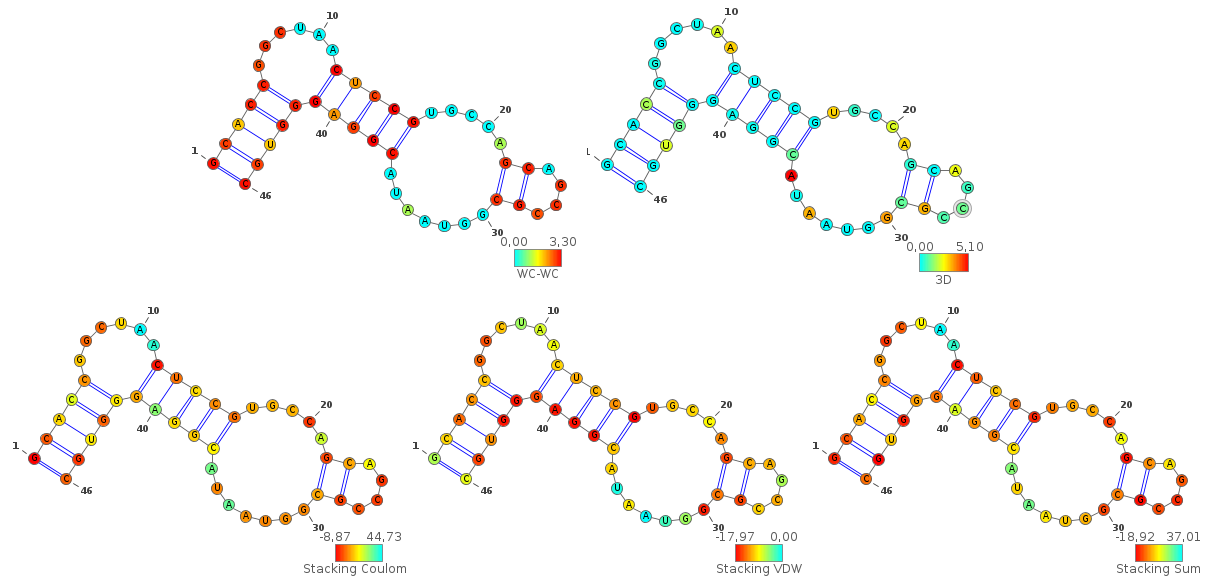
\includegraphics[scale=0.6]{./pictures/varna3.png}
\caption{Figures with average secondary structure coloured by the values of computed parameters, generated by MINT using the  VARNA \cite{Blin2009} program.}
\label{varna}
\end{figure}


\newpage

\item Files needed for visualization using external tools (see section \ref{Visualization} for details):
\begin{itemize}
\item \texttt{\_RNAStructML.xml} 
\item \texttt{\_2D.pdb}
\item \texttt{\_3D.pdb}
\item \texttt{\_coulomb.pdb}
\item \texttt{\_VDW.pdb}
\item \texttt{\_stacking\_sum.pdb}
\item \texttt{vmd\_run.tcl}
\end{itemize}
\end{itemize}

Detailed description of the visualization procedures can be found below.


\section{Workflow}
Figure \ref{ProgramScheme} shows the structure of the program. First, the program reads in the conformation and finds all hydrogen bonds between nucleotides. They allow to determine secondary and tertiary structures and subsequent classification of the secondary structural motifs. The main outcome is a set of statistical descriptors of the given RNA structure. In this document we  describe the algorithm, inputs and outputs of the program. 

\begin{figure}[h!]
\centering
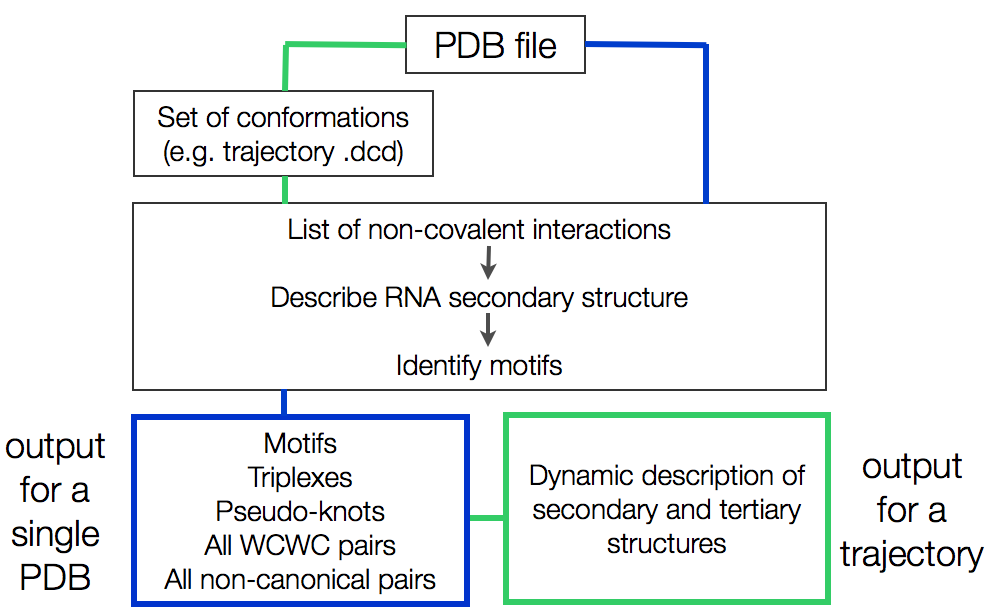
\includegraphics[scale=0.4]{./pictures/workflow.png}
\caption{Main function implements the analysis of a single frame. In the case of a trajectory, the function reads-in the list of nucleotides from a given PDB and then refreshes the atom coordinates while reading the next frame. Additionally, the script splits the trajectory between CPUs and runs separate processes, what  accelerates the calculations.}
\label{ProgramScheme}
\end{figure}

\subsection{Loading the RNA structures}
The script is entirely written in {\tt Python} programming language (\url{http://python.org}). Its modular structure enables applying it in various programming contexts. Reading the PDB file is implemented by BioPython package (\url{http://biopython.org/wiki/Main_Page}), providing a complete objective structure for dealing with PDBs. The basic object is an atom that despite the name and number is described with spatial coordinates. A molecule consists of the residues that have such attributes as a name, a number and a list of atoms. This allows fast and easy access to the nucleotides, atoms and their coordinates.

\subsection{Hydrogen bonding}
\label{Hbond-section}
A hydrogen bond is a basic interaction responsible for creating the secondary and tertiary structures of nucleic acids. A typical definition of a hydrogen bond pertains to a non-covalent interaction when a hydrogen atom is placed close to its acceptor.

Both the distance and the angle (Figure \ref{hbond}) depend on the characteristics of the donor and acceptor. Theory states that all hydrogen bonds are almost linear (around $175^\circ$) \cite{Guerra2000}. For biological molecules the hydrogen bond distance should be typically between 2,80 and 3,06 \AA\ between a donor and acceptor, which gives 1,60 and 1,80 \AA\ between an acceptor and hydrogen. The user can decide which distance will be measured by {\tt MINT} using the \texttt{h\_bond\_atom} parameter.
Other user defined parameters are: the minimal angle and the maximal length of a hydrogen bond. The default values of the \texttt{h\_bond distance} (4 \AA) and the \texttt{h\_bond\_angle} ($140^\circ$) are in consistence with distance calculated between donor and acceptor atoms. 


\begin{figure}[h!]
\centering
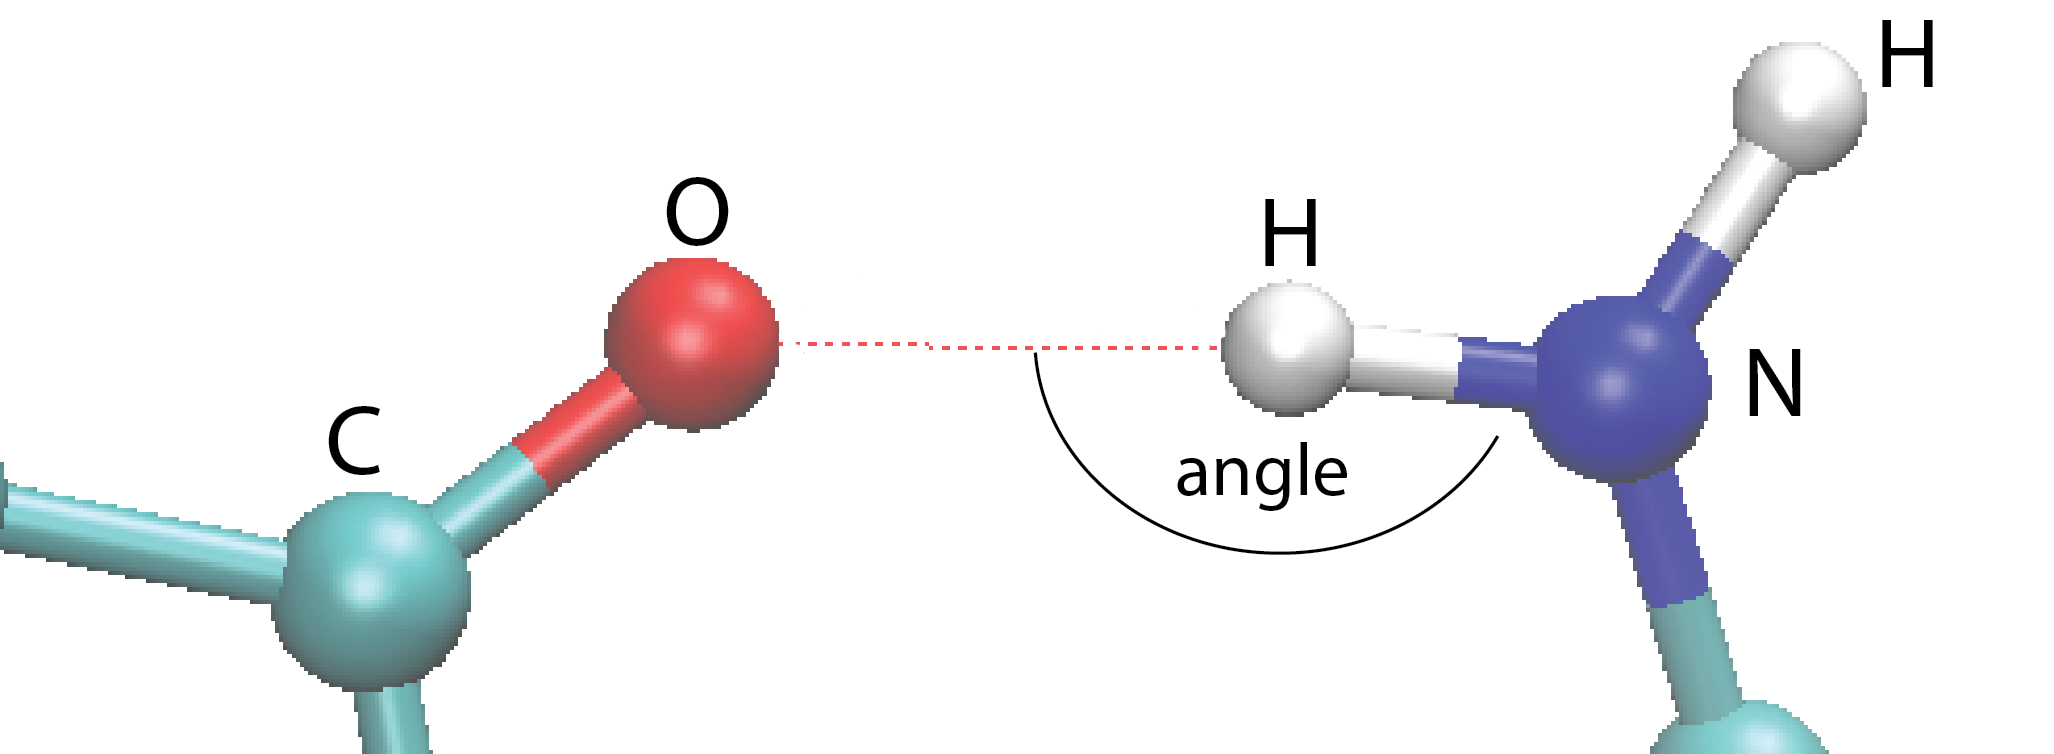
\includegraphics[width = 10cm]{./pictures/hydrogen_bond_2.png}
\caption{The scheme of the hydrogen bond with the nitrogen atom as a donor and the oxygen atom as an acceptor.}
\label{hbond}
\end{figure}

\subsection{Donors and acceptors}
\label{donrsandacceptors}
To analyze the structures we have defined a list of possible acceptors and donors for all nucleotides of RNA and DNA. Following the classification by Leontis and Westhof \cite{Leontis2002} the acceptors and donors are assigned to the edges of the nucleotide, as shown in Figure \ref{Edges}. This classification is stored in the {\tt table\_nucleotides} .csv file and may be edited by the user. 

{\tt MINT} determines the interacting edges of every pair of nucleotides. Several atoms are situated in the corners of the nucleotides and participate in more than one edge. In that case, the program first classifies all the remaining bonds and chooses the prevailing edge. If there is only one hydrogen bond, both edge names are returned. 

\begin{figure}[h!]
\centering
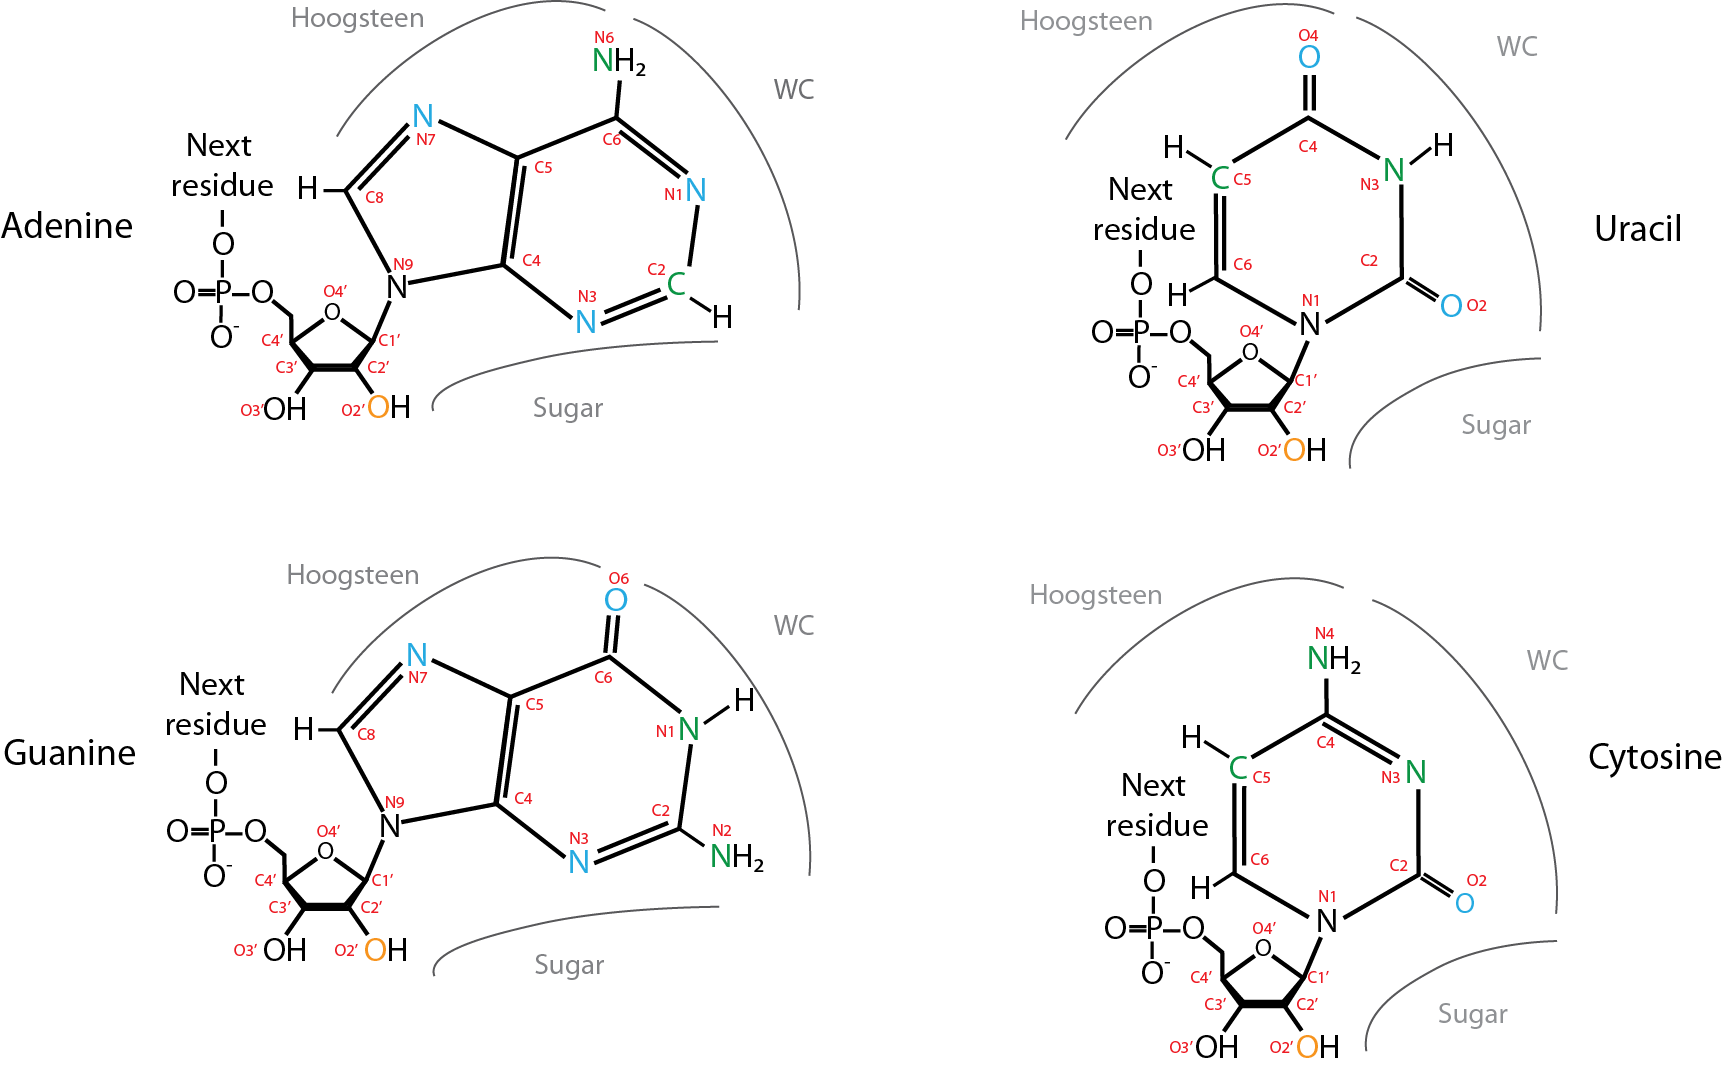
\includegraphics[width = 14cm]{./pictures/donors_acceptors_nucleotides.png}
\caption{Nucleotides with selected edges, donors (green) and acceptors (blue). WC corresponds to WC edge.  \cite{Lescoute2006}.}
\label{Edges}
\end{figure}

% Pairs
{\tt MINT} checks all the donors against all of the acceptors of all possible pairs of all of the nucleotides in the molecule. In order to decrease the computational time, we assumed that the partner for a given nucleotide can be found only among its closest neighbors. The exact distance is defined by the user in the {\tt cutoff} parameter. Knowing the atoms creating hydrogen bonds, the program can determine the interacting edges.

\subsection{Modified nucleotides}
Modified nucleotides are found in almost all tRNAs, sRNAs, mRNAs and other functionally important RNA molecules. Several of them are presented in the Figure \ref{ModifiedNucleotides}. 
\begin{figure}[h!]
\centering
\begin{center}
\subfigure[2MG]{
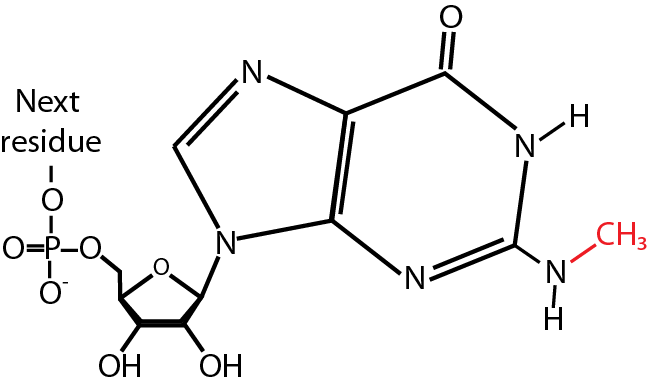
\includegraphics[scale=0.8]{./pictures/modified_1.png}}
\subfigure[OMC]{
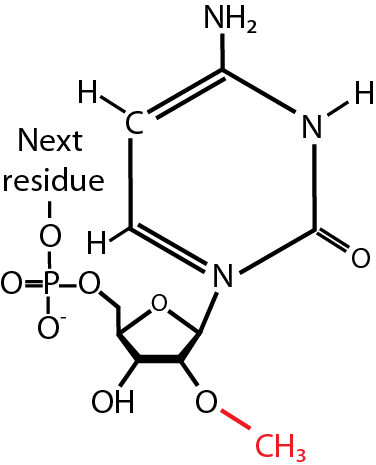
\includegraphics[scale=0.8]{./pictures/modified_2.png}}
\subfigure[YYG]{
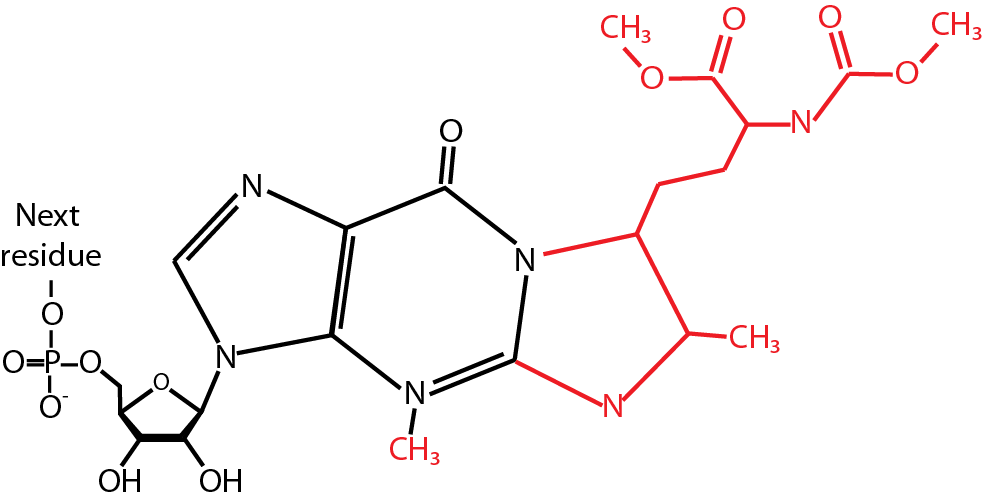
\includegraphics[scale=0.8]{./pictures/modified_3.png}}
\end{center}
\caption{Three out of ten modified nucleotides present in tRNA structure (PDB: 1ttt) along with their PDB ID. Red color indicates atoms that are not present in normal nucleotides. }
\label{ModifiedNucleotides}
\end{figure}

There are about 600 modified RNA nucleotides in the PDB database, but for most of them there are no force field parameters. We provide the VDW parameters and partial atomic charges, necessary for stacking interactions computation, for 107 naturally occurring modified nucleotides developed by Aduri et al~\cite{Aduri_2007}. For these nucleotides, we have also assigned their atoms to distinct edges: the WC edge, the Hoogsteen edge, the sugar edge and to the edge named modification (see section \ref{donrsandacceptors} for details about edge classification). 

Atom in modified nucleotide is assigned into the same edge as in unmodified. Addition of no more than one heavy atom to the nitrogenous base was also classified into the same edge as base atom. 2'O methyl carbon was assigned to the sugar edge. All other atoms present in the modified nucleotide but not in the original one were classified into the modification edge.

When {\tt MINT} encounters a modified nucleotide - it looks for the appropriate parameters in the {\tt table\_nucleotides}. Not having parameters, {\tt MINT} uses the \texttt{list\_of\_modified\_nucs} to find the natural ancestor of the modification. Atoms common for modified and its natural ancestor are assigned analogously to the original nucleotide, the rest is assigned to the modification edge. With lack of the charges and VDW parameters values of the stacking interaction energy are set to 0.

User can add new modified nucleotides. If one knows forcefield parameters for MD simulation, they can be successfully adopted to the {\tt MINT} parameters format. If you want to add your own modification to the {\tt MINT} parameters: you should edit the {\tt table\_nucleotides} file and add a new row with the name of your residue and appropriate names of atoms in the donors and acceptors columns. Than you should also modify the \texttt{table\_charges} file. For every atom that should be considered in stacking computations you have to add a row with the name of the residue, charge, VDW radius and well depth parameter. For details see sections \ref{Hbond-section} and~\ref{stacking-section}.

\subsection{Basepairs geometric isomerism}
For detected pairs the geometric isomerism of their glycosidic bonds is computed. The program measures the torsion angle formed by the four atoms (C1', N1 in pyrimidines and C1', N9 in purines) and depending on its value a {\it cis} or {\it trans} conformation is denoted (Figure \ref{Conf}).

\begin{figure}[h!]
\begin{center}
\subfigure[Cis]{
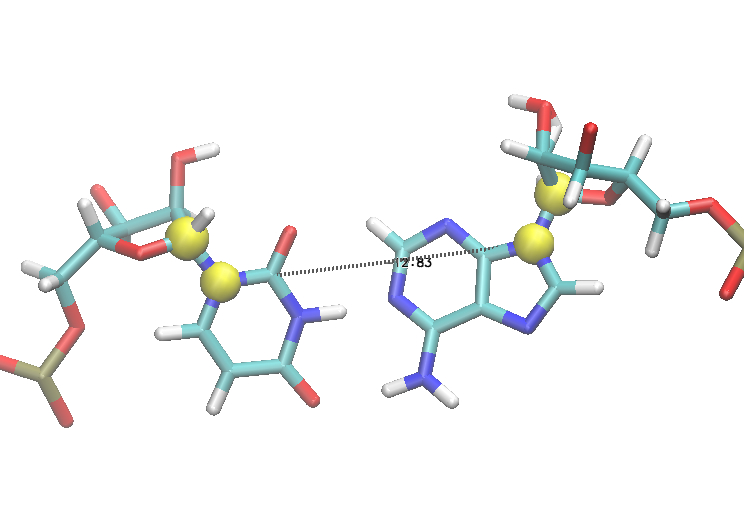
\includegraphics[width=6.5cm]{./pictures/torsion_angle_cis.jpg}}
\subfigure[Trans]{
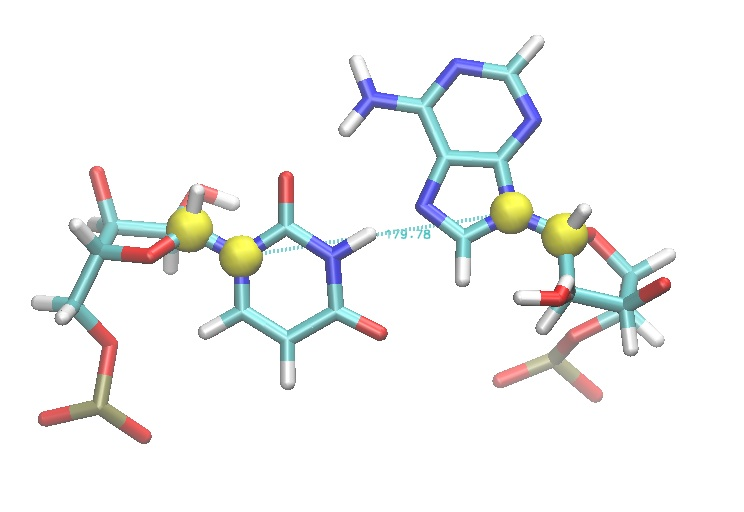
\includegraphics[width=6.5cm]{./pictures/torsion_angle_trans.jpg}}
\end{center}
\caption{Yellow spheres correspond to C1' and N1 atoms in pyrimidines and N9 atoms in purines. The torsion angle created by these four points determines the geometric isomerism of the two nucleotides creating a pair. }
\label{Conf}
\end{figure}

%Stacking interactions
\subsection{Stacking}
\label{stacking-section}
Stacking is an important non-covalent interaction contributing to the stability of both double helix and single stranded structures of nucleic acids \cite{Hobza2008}. It is suspected to be especially important for RNA molecules. In tRNA only a half of the nucleotides form a helix, but about 90\% of residues is stabilized by stacking \cite{Bloomfield1999}. 
\begin{figure} [h!]
\begin{center}
\subfigure[]{
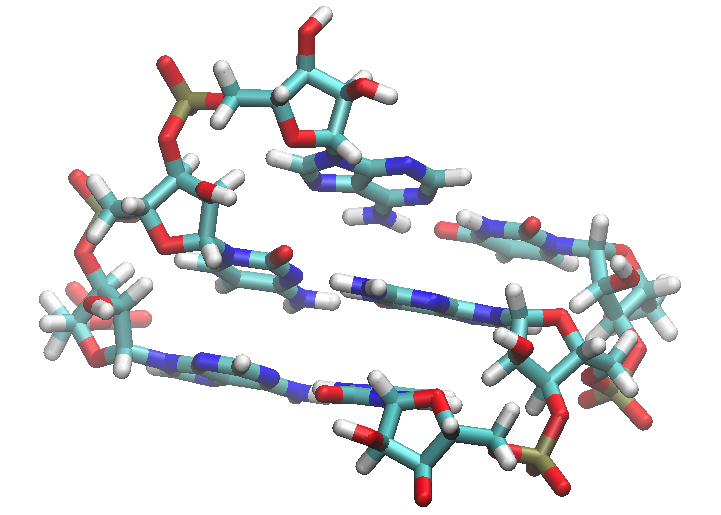
\includegraphics[width=5.0cm]{pictures/stacking1.png}}
\subfigure[]{
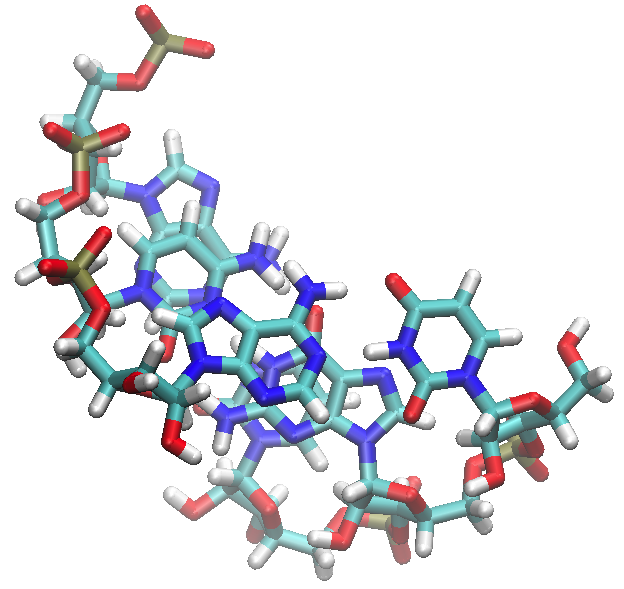
\includegraphics[width=5.0cm]{pictures/stacking2.png}}
\subfigure[]{
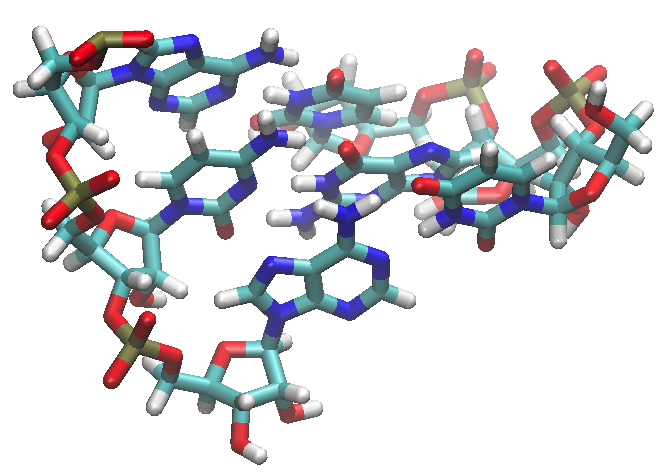
\includegraphics[width=5.0cm]{pictures/stacking3.png}}
\caption{Three-pairs of an RNA helix seen from different angles to expose  stacking between parallel bases.}
\label{StackingHelix}
\end{center}
\end{figure} 
Generally, stacking occurs between aromatic rings, in nucleic acids between the nucleobases. There is a general belief that stacking results from contact of the electron $\pi$-systems. Stacking is also supported by the three phenomena: Van der Waals (dipole or induced-dipole attractions), electrostatic and solvation effects. It seems to be more important in folding of nucleic acids than proteins because nucleotide bases are more polarizable than most amino-acids. 

%In order to measure stacking separately of hydrogen bonding the experiments where conducted with a helix terminated with a single nucleotide. Presence of the unpaired nucleotide  stabilizes the entire helix. Sites are uneven, for DNA the on the $5\prime$ site of the helix is more favorable energetically than the other one, but for RNA the $3\prime$ is \cite{Kool2001}. Experimental studies indicated ability of stacking among natural bases is the strongest between two purines, than purine-pyrimidine and pyrimidine-pyrimidine \cite{Guckian2010}.

It is believed that stacking is one of the best represented terms in molecular modeling. 
Especially with the Amber atomic charges which are fitted to molecular electrostatic potentials~\cite{Hobza2008}. It was shown that calculations using the empirical potentials consisting of the Lennard-Jones VDW and Coulombic terms with atom-centered point charges were able to reproduce the {\it ab initio} stacking energy over the major portion of the conformational space~\cite{Leszczynski2002}.
\v{S}poner et al. in multiple works~\cite{Carter2000,Sponer1997, Base1996, Hobza1995} compared {\it ab initio} energies for about 300 geometries of stacked base dimers with data obtained using empirical potentials. The agreement between these methods is remarkable, which suggests that calculations based on empirical potentials provide an excellent approximation of the stacking interaction energy between nucleotides. 

We estimate stacking between two bases by calculating the energy of electrostatic ($U_{el}$) and Van der Waals ($U_{VDW}$) interactions applying the equations used in molecular mechanics:
\begin{equation}
U_{el} = k \sum{\frac{q_i q_j}{r_{ij}}}
\end{equation}

\begin{equation}
U_{VDW} = 4 \epsilon_{ij} \sum{ \left[ \frac{1}{4} {\left( \frac{r_0}{r_{ij}} \right) }^{12} - \frac{1}{2} {\left( \frac{r_0}{r_{ij}} \right) }^{6} \right]}
\end{equation}
The sums consist of all pairs containing atoms from nucleobases $i$ and $j$. $k$ denotes the Coulomb constant ($k = \frac{1}{4 \Pi \epsilon_0}$), $q$ is the partial atomic charge of the atom, $r_{ij}$ is the distance between considered atoms, $\epsilon_{ij}$ is the depth of the Lennard-Jones potential well for atoms $i$, $j$ ($\epsilon_{ij} = \sqrt{\epsilon_{ii}\epsilon_{jj}} $) and $r_0$ is the sum of Van der Waals (VDW) radius of atoms  $i$ and $j$.
We provide the VDW well depth parameters and partial atomic charges from the Amber~\cite{Wang2000} and Charmm~\cite{Mackerell2000,Foloppe2000} force fields. A set of parameters and charges may be also defined by the user in the file \texttt{table\_charges} file. Only the nucleobases that are closer than the user defined cutoff (\texttt{cutoff\_stacking}) are considered in the stacking calculations. The unit for energy values obtained from described calculations is $kcal/mol$. 

The electrostatic term, depending on the orientation of bases' dipole moments, may be attractive or repulsive regardless the bases are parallel or not to each other. While the VDW energy component is almost always favorable regardless base orientation.
What is more, the shape of nucleotides and method used for calculation the VDW energy, ensure that the lowest VDW values are obtained for parallel nucleotides which the biggest overlap.
It was also visible in our test calculations.
Thus we recognize two nucleotides as stacked, if their VDW energy is lower than \texttt{vdw\_cutoff\_stacking} parameter. 
The default value is $ -0.5 kcal/mol$.
It was found by trial and error and seems to be appropriate for the nonmodified nucleobases.


%\subsection{Anion-$\pi$ contacts} Following recent research on the types of non-covalent contacts in RNA molecules, \texttt{MINT} also analyzes the anion-$\pi$ - contacts and hydrogen bonding interactions, per nucleotides and in pairs \cite{Auffinger2013}. Detection of these interactions is based on the distance between the oxygen atom and the center of the mass of a nucleobase ring. 

\subsection{Ion-$\Pi$ interaction}
In biomolecules such as RNA, proteins and their complexes the non-covalent interactions play significant role. Hydrogen bonds are the most known non-covalent interactions but not the only one. For example the cation-$\Pi$ interactions, namely the non-covalent bonding between a monopole (cation) and a quadrupole ($\Pi$ system), seems to play important role in proteins structure.
Similar interaction was reported for the RNA molecules, but it was found that nucleic acid aromatic systems prefer to interact with anionic rather than cationic species~\cite{Auffinger2013}. 
{\tt MINT} allows to search for anion-$\Pi$ interactions involving RNA backbone phosphate groups and nucleotides bases. The example is shown in Figure \ref{stackingPiExamples}.
\begin{figure}[h!]
\begin{center}
\subfigure[]{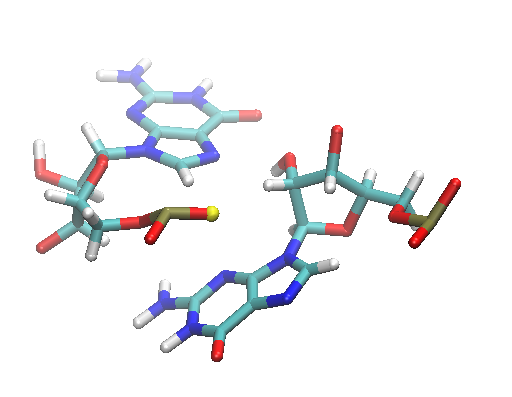
\includegraphics[scale = 0.3]{pictures/stacking_pi_1.png}
\label{stackingPiexample1}}
\subfigure[]{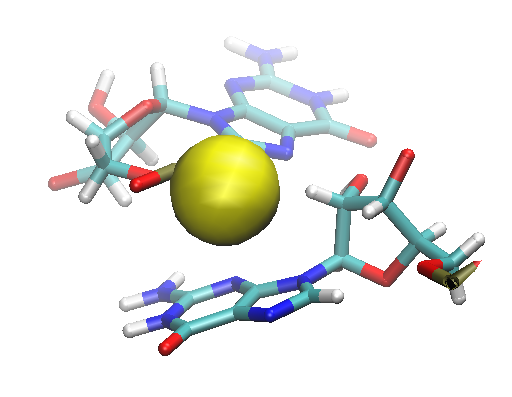
\includegraphics[scale = 0.3]{pictures/stacking_pi_2.png}
\label{stackingPiexample2}}
\subfigure[]{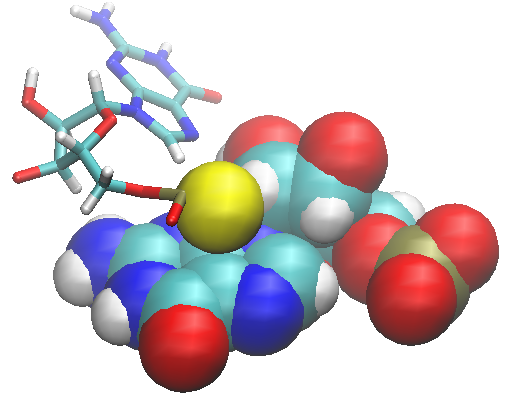
\includegraphics[scale = 0.3]{pictures/stacking_pi_3.png}
\label{stackingPiexample3}}
\caption{Three representations of the oxygen atom (yellow) "stacking" over the guanine base. The yellow sphere in the \label{stackingPiexample1} picture corresponds to the real VDW radius.}
\label{stackingPiExamples}
\end{center}
\end{figure}
Potentially interacting systems are recognized if distance between phosphate atom and nucletide base centre of mass is lower than \texttt{OP\_stacking\_distance\_cutoff} parameter (default distance is $ 5 \AA$). If the ion-$\Pi$ stacking is detected, the energy of interaction between phosphate atom and nucleotide base is calculated in the same way as in the stacking between two nucleobases. 

\subsection{Representation of the RNA motifs}
Having all WC pairs, a list-representation of the RNA secondary structure is created. We assume that one nucleotide can have only one WC partner. If the second WC partner is encountered, all three nucleotides are denoted as a triplex. The index of the list represents the nucleotide number the stored value is the index of its WC partner. The list is easy-interpretable when the arcs connecting the pairs are drawn as  presented in Figure \ref{SecondaryStructureList}. 

\begin{figure}[h!]
\centering
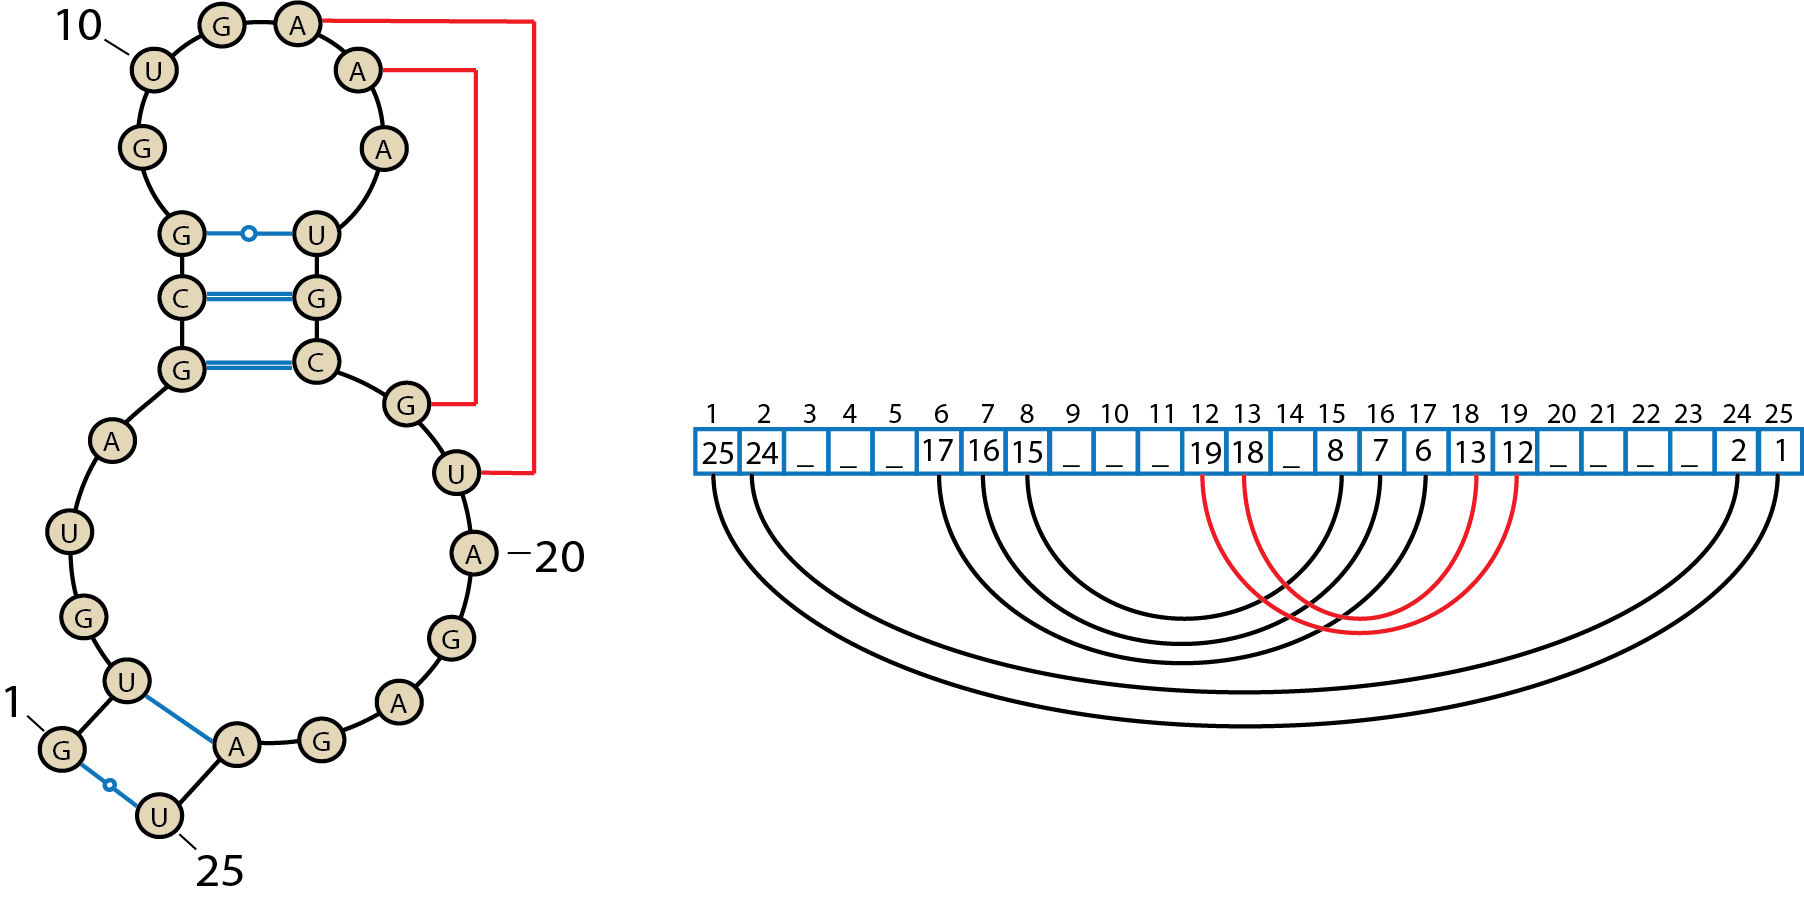
\includegraphics[width = \textwidth]{./pictures/PseudoKnotArchs.png}
\caption{Secondary structure of an exemplary RNA molecule and its list-representation. Red lines correspond to the WC interactions creating a pseudo-knot.}
\label{SecondaryStructureList}
\end{figure}

\paragraph{Pseudo knots}
The list-representation contains also the information about the non-secondary motifs. The pseudo-knot is formed by the WC interactions but creates three-dimensional folds as shown in Figure \ref{PseudoKnot}. Our program detects the pseudo-knot fold when the arcs intersect. A pseudo-knot is a symmetric structure -- both the three pairs 6--17, 7--16, 8--15  in Figure \ref{SecondaryStructureList} form the pseudo-knot as well as the two pairs: 12--19, 13--18. The natural way of solving this conflict is to choose the shorter list, in this case the pairs 12--19 and 13--18.  
\begin{figure}[h!]
\begin{center}
\subfigure[Tertiary structure]{
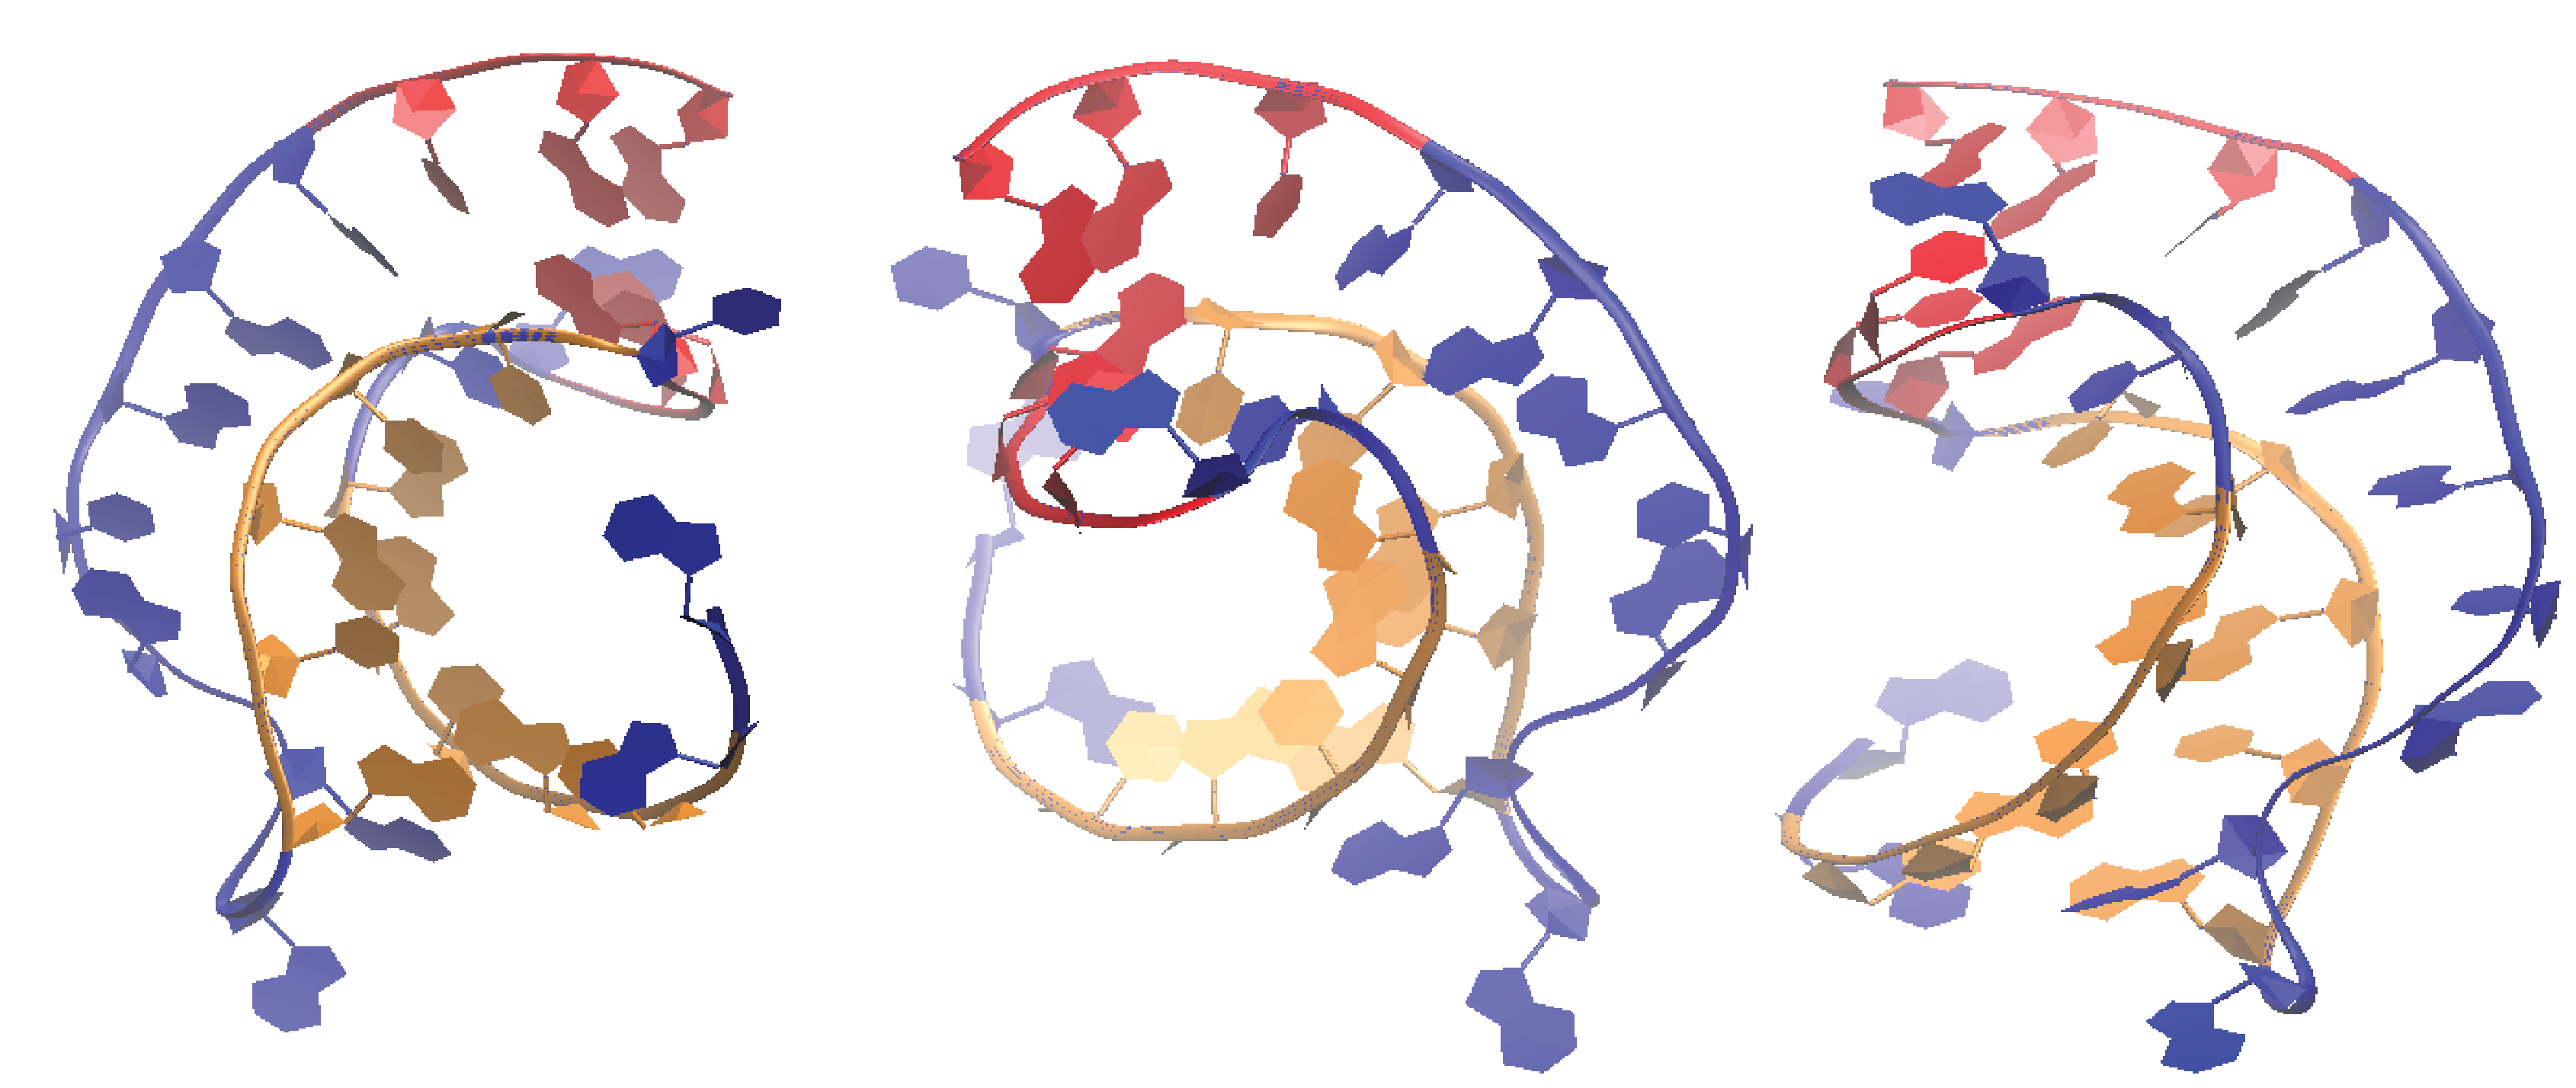
\includegraphics[width=12.5cm]{./pictures/pseudo_knot_combo.png}}
\subfigure[Secondary structure]{
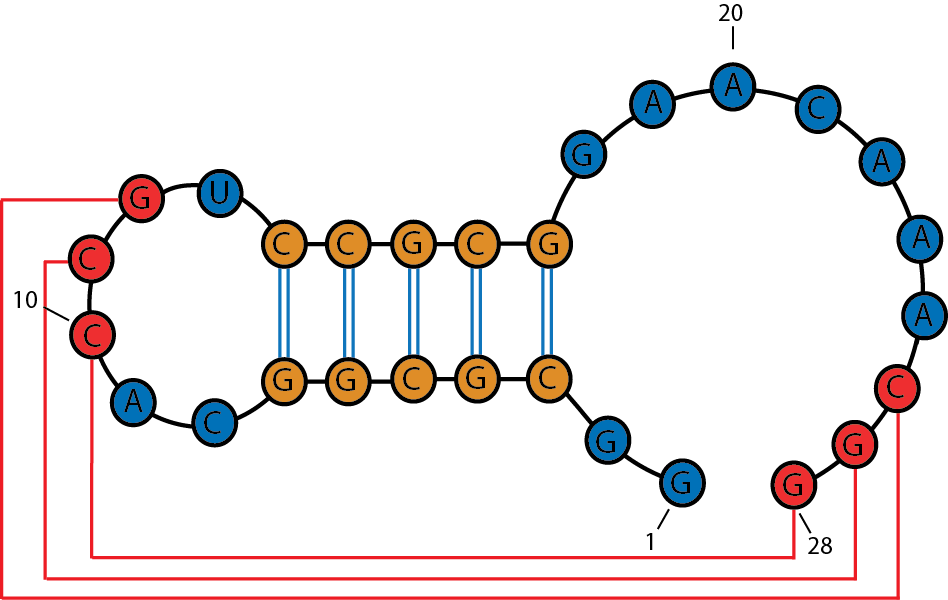
\includegraphics[width=6cm]{./pictures/pseudo_secondary_structure.png}}
\end{center}
\caption{An example of RNA structure with a pseudo-knot seen from three different angles. Nucleotides colored in red create a pseudo-knot, orange form a helix and blue refer to loops (PDB id: 437d).}
\label{PseudoKnot}
\end{figure}
\newpage
After detecting all pairs, and creating the list, {\tt MINT} finds all pseudo-knots and erases them from the list by putting the \texttt{None} value. Next, it looks for all kinds of motifs, that are defined as a set of unpaired nucleotides with the surrounding pairs as it is show in Figure \ref{MotifDesc}.

\begin{figure}[h!]
\centering
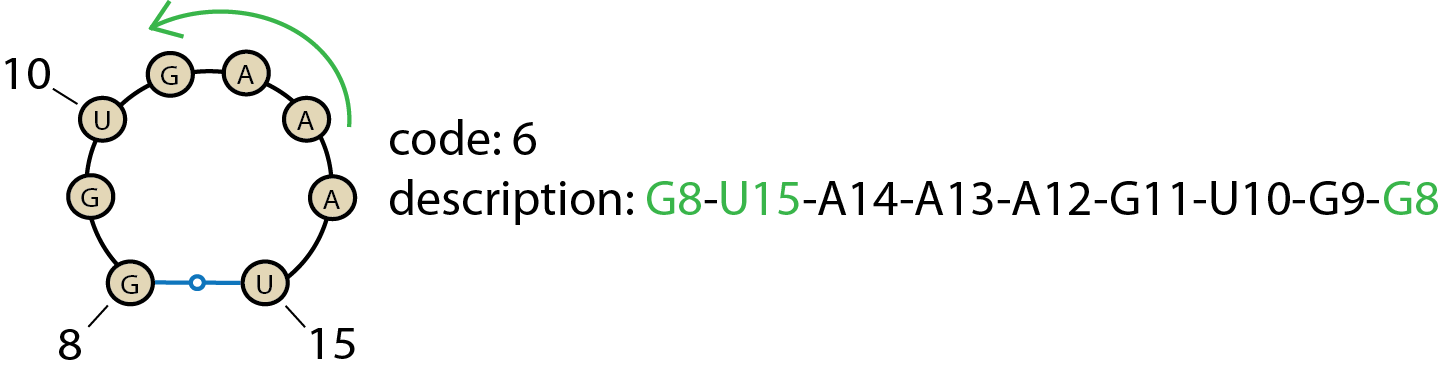
\includegraphics[width = \textwidth]{./pictures/motifs_description.png}
\caption{Program denotes the first pair (shown in green) and than list of unpaired nucleotides. Nucleotides are listed in accordance with the counter-clockwise direction.}
\label{MotifDesc}
\end{figure}

\begin{table}
\caption{RNA secondary structure motifs}
\label{RNAsecondaryStructures}
\begin{tabular}
{ >{\centering} p{5.5cm} >{\centering} p{5.5cm} >{\centering} p{5.5cm}}
&& \tabularnewline
 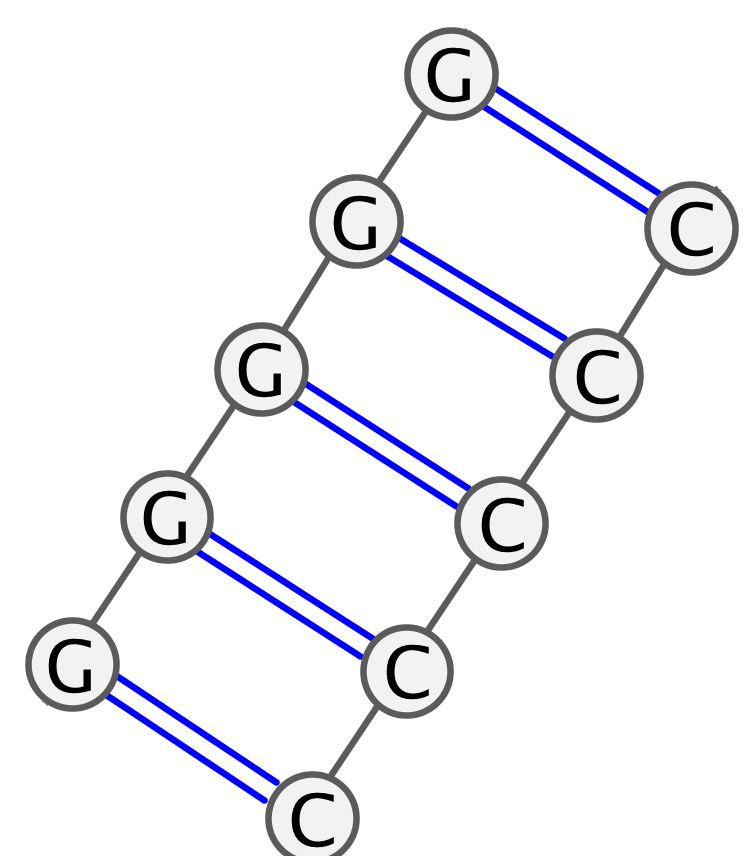
\includegraphics[width=4.5cm]{./pictures/helix_varna.PNG}  \linebreak Helix 
 & 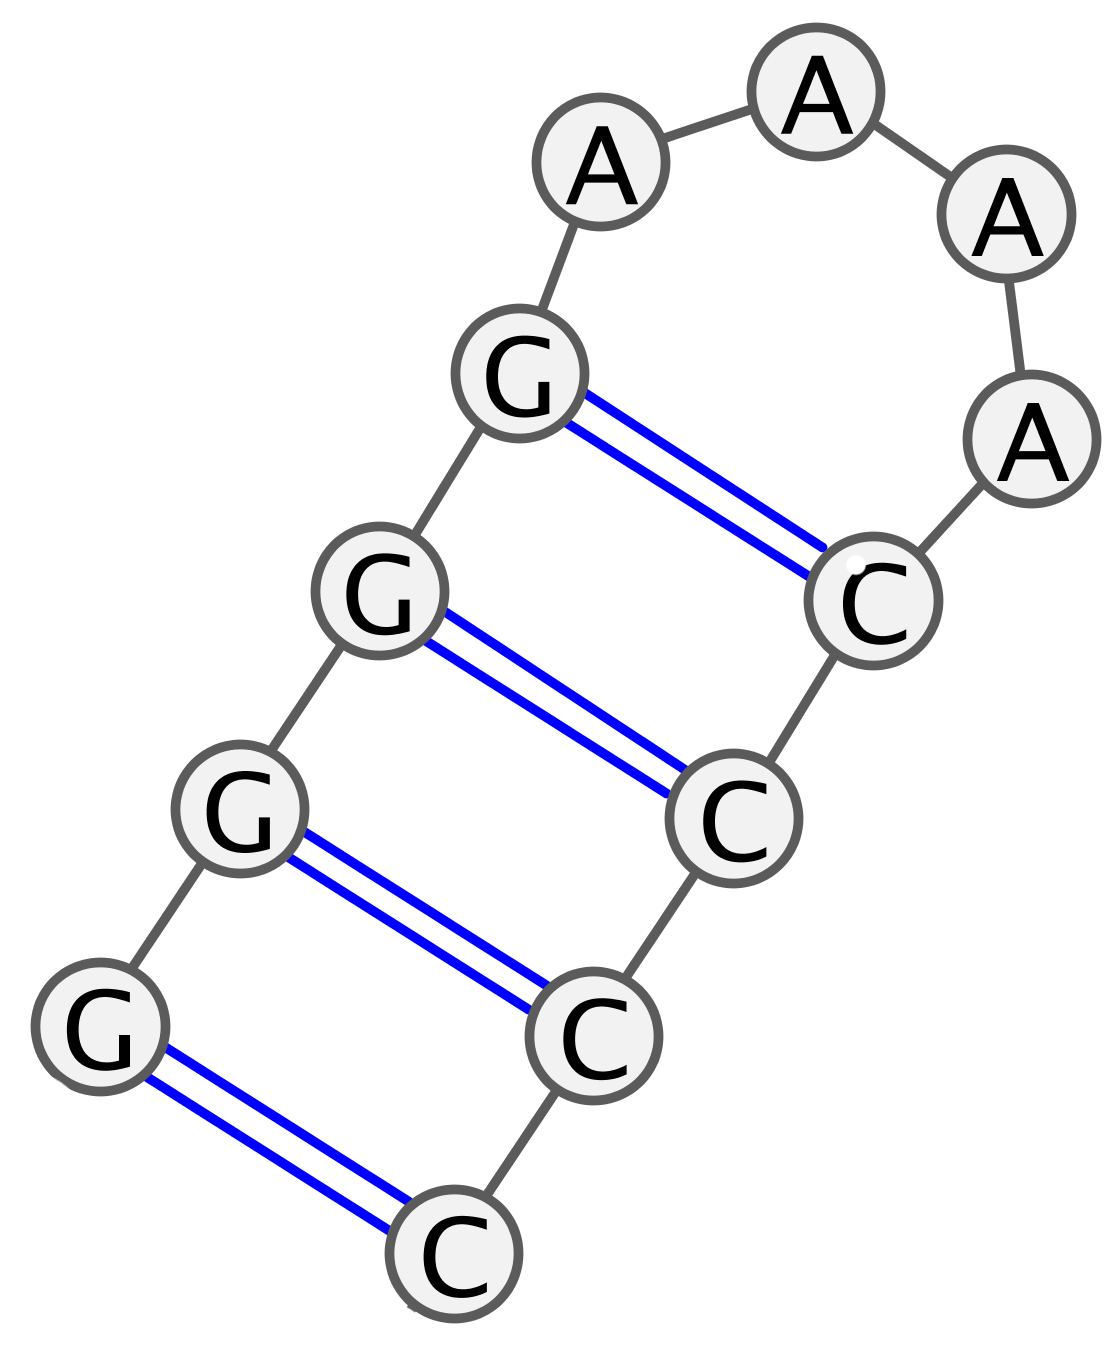
\includegraphics[width=4.5cm]{./pictures/hairpin_varna.PNG}  Hairpin loop \linebreak (code: 4) &  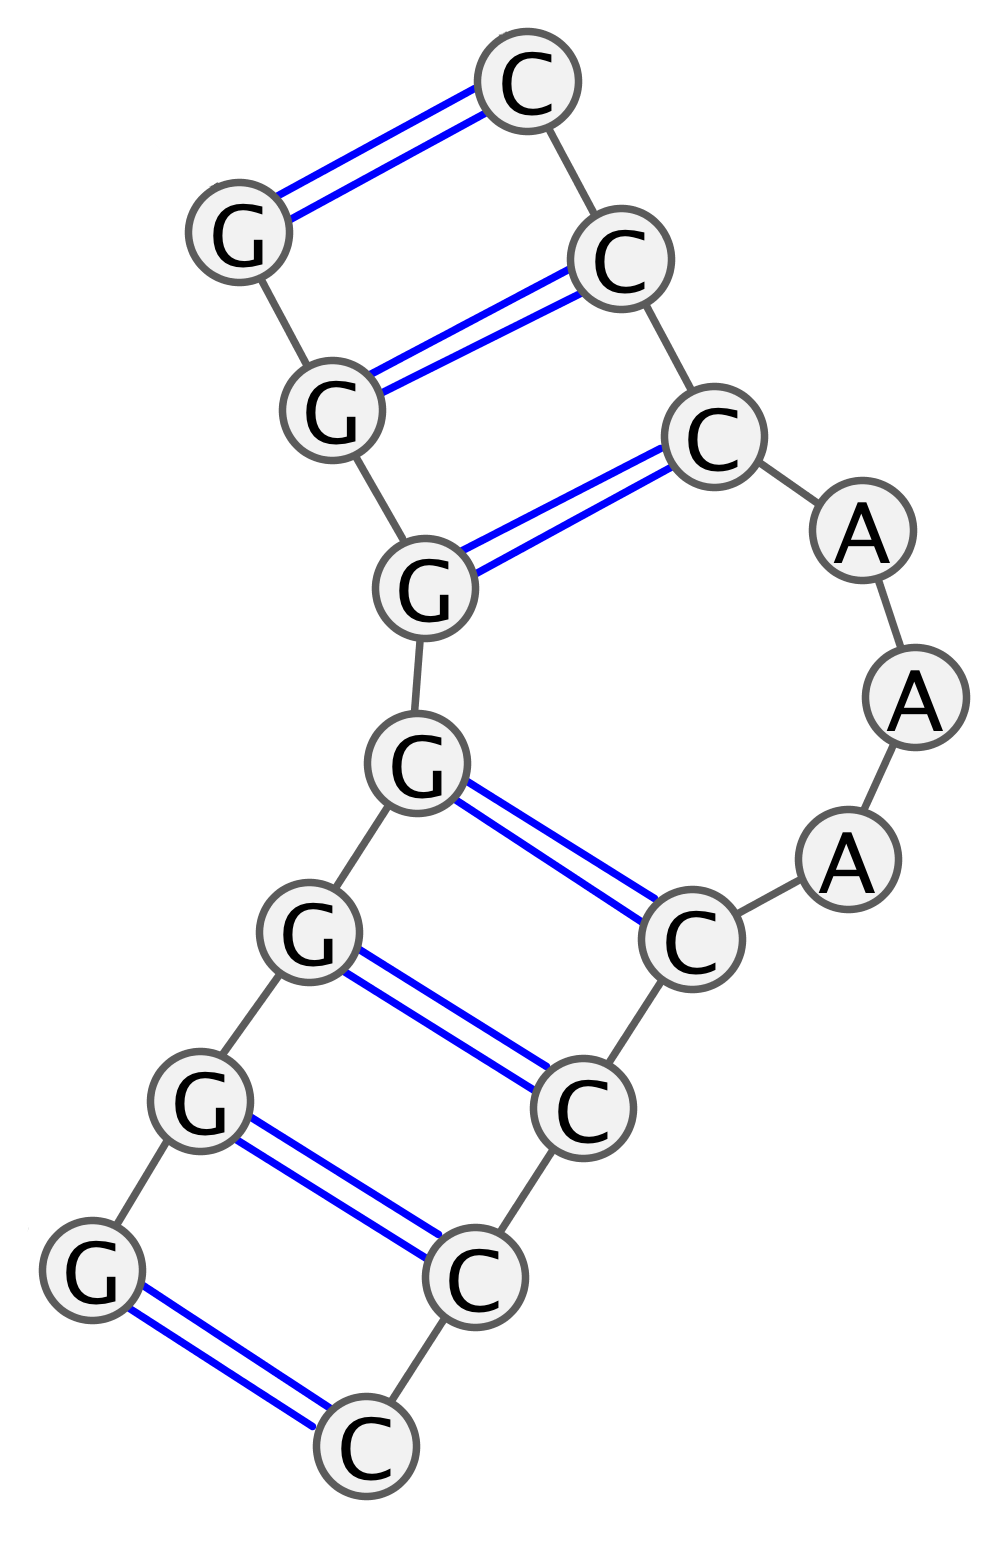
\includegraphics[width=4.5cm]{./pictures/bulge_varna.PNG} Bulge loop\linebreak  (code: 0--3) \tabularnewline
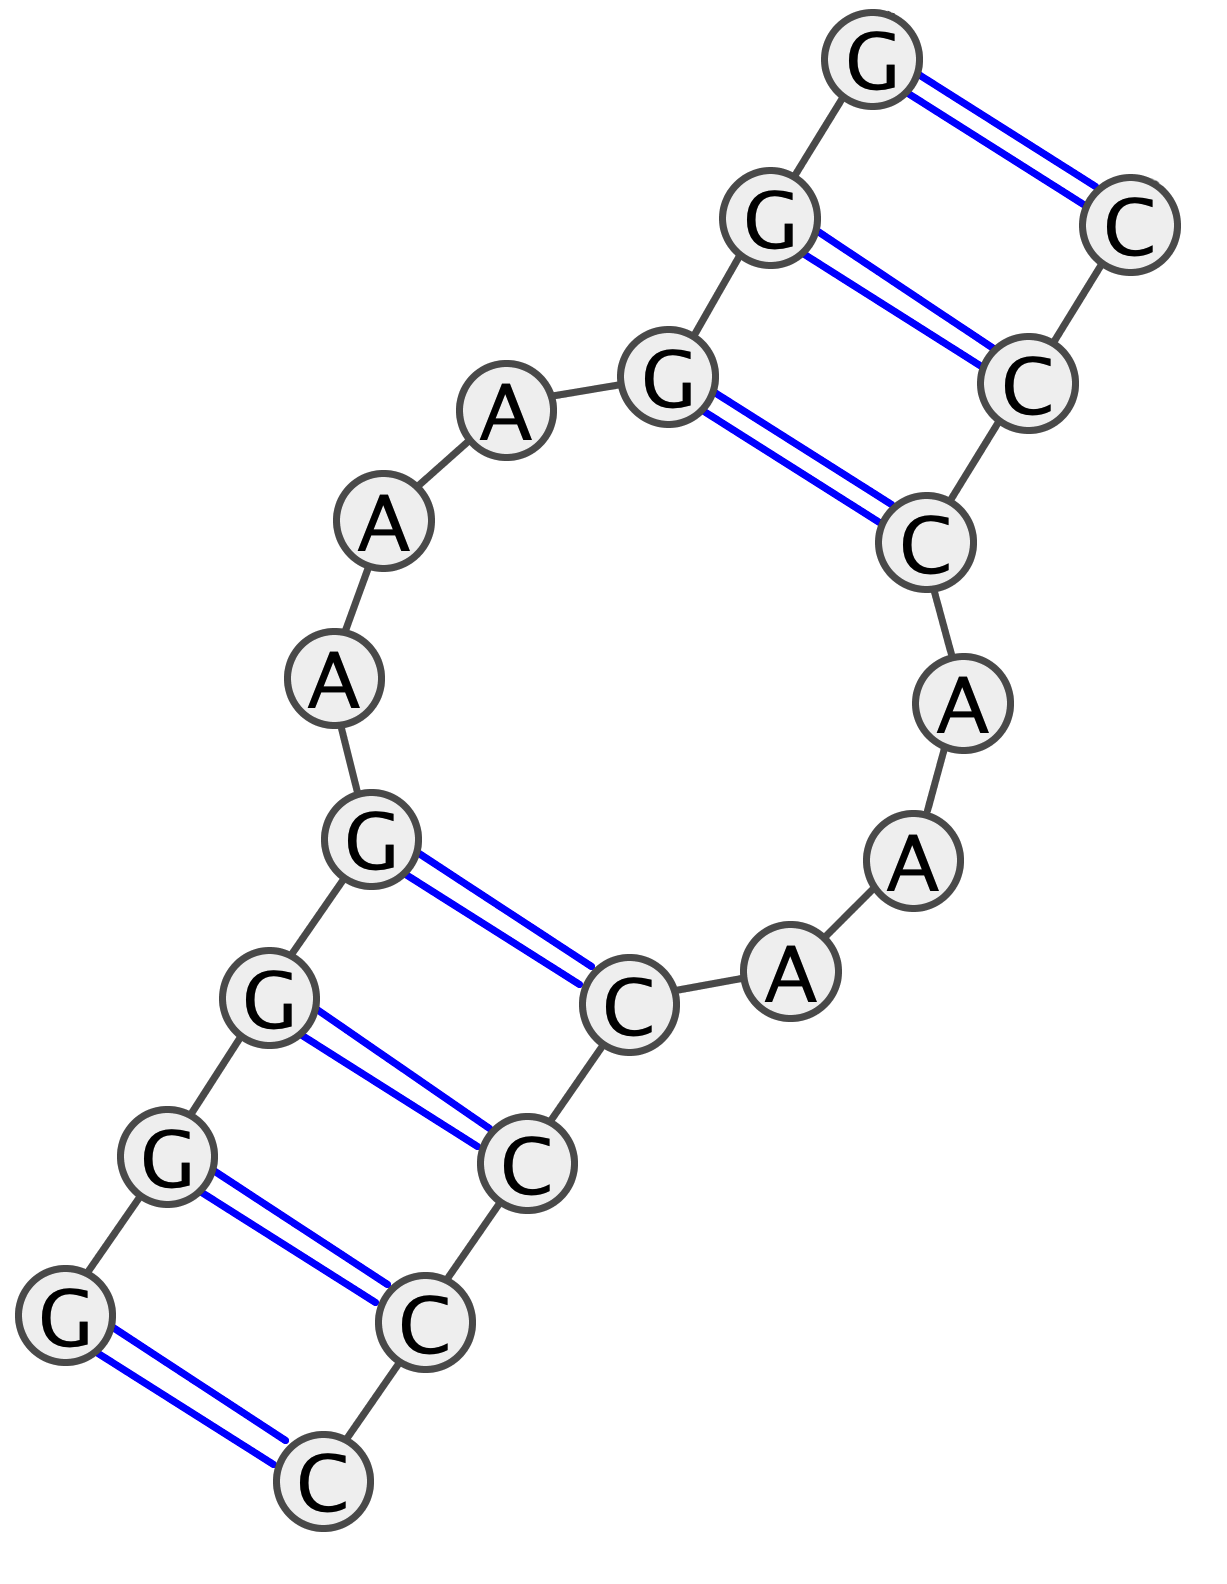
\includegraphics[width=5cm]{./pictures/interior_varna.PNG} Interior loop \linebreak  (code: 3--3) & 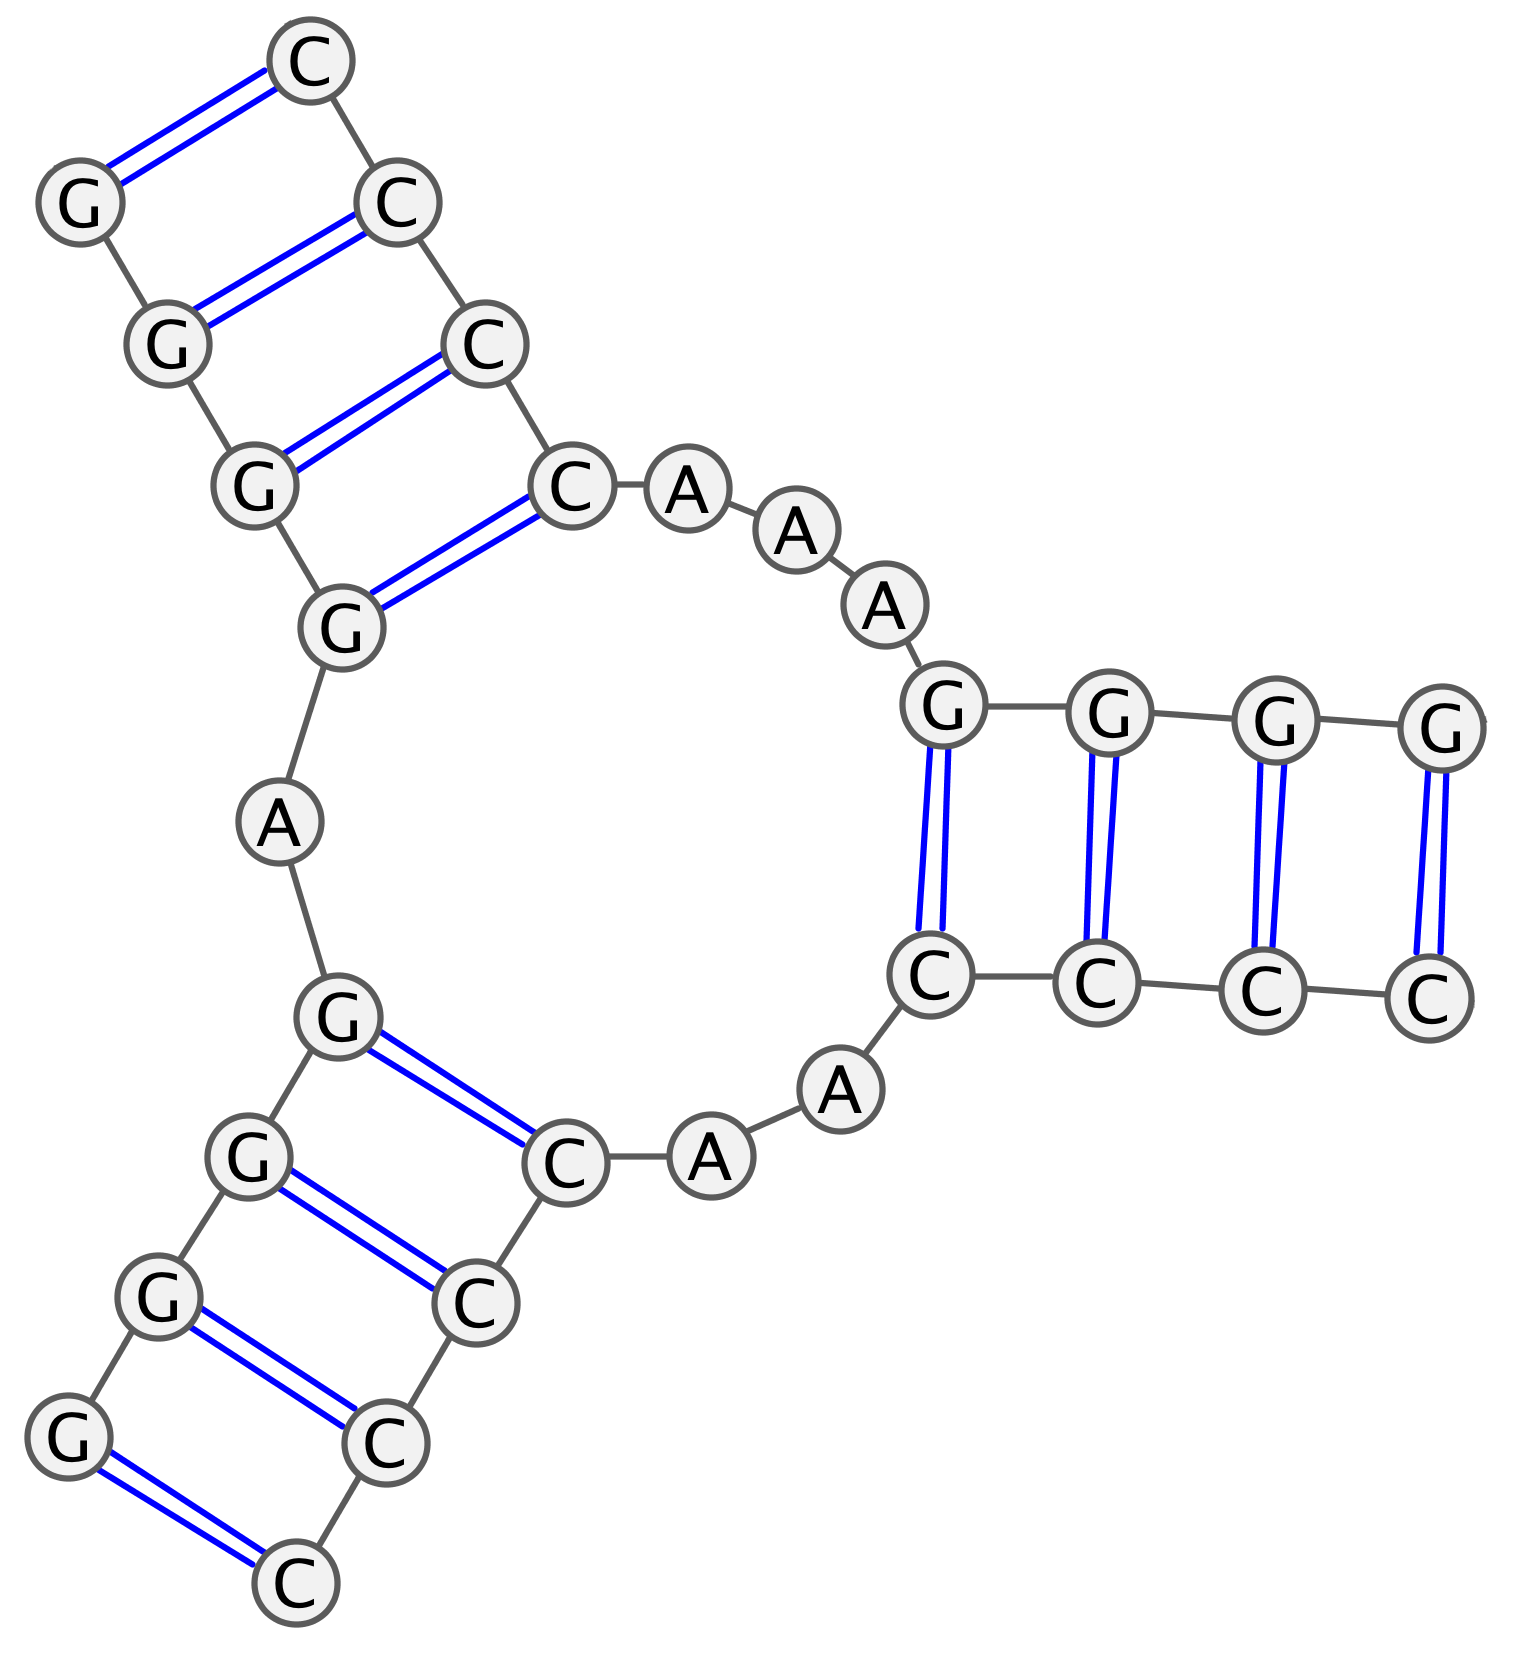
\includegraphics[width=5.5cm]{./pictures/multibranched_varna.PNG} Multi-branched loop\linebreak (code: 2--3--1) & 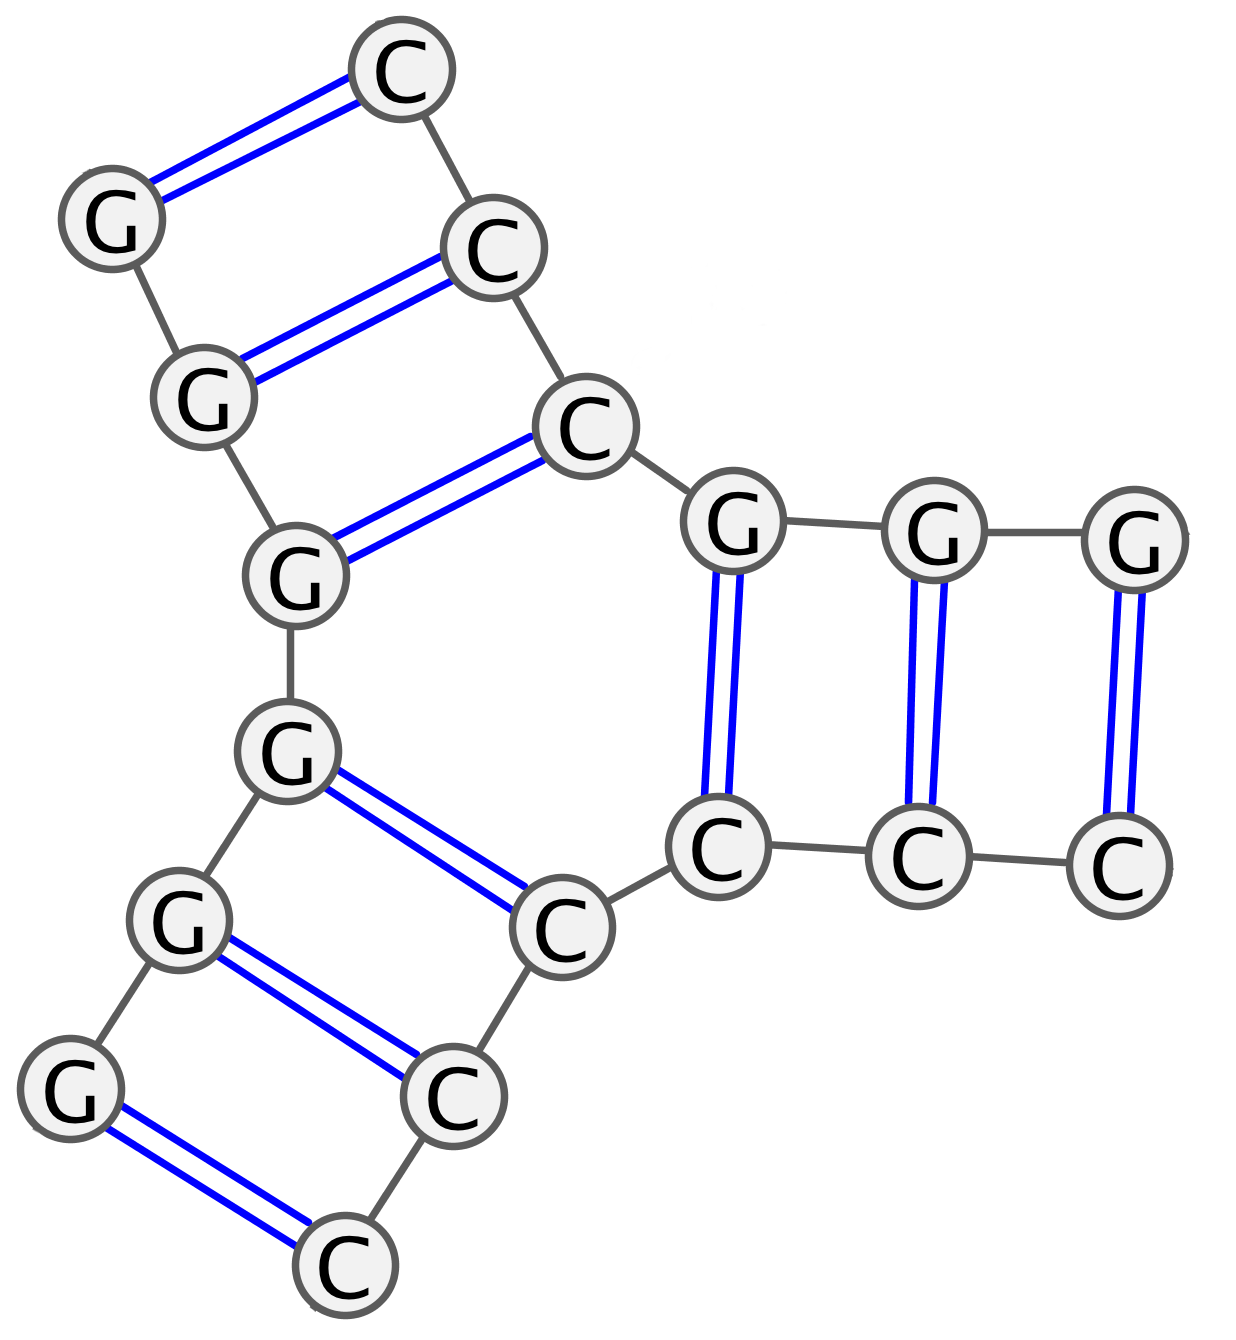
\includegraphics[width=5cm]{./pictures/junction_varna.PNG} 3-way junction\linebreak (code: 0--0--0)  \tabularnewline
&& \tabularnewline
\end{tabular}
\end{table}

\newpage

\paragraph{RNA motifs} \label{RNA_motifs} nomenclature (loop, bulge, junction) can be inaccurate and misleading. The program uses the numerical description of the motifs that is understandable for people. The numbers correspond to the numbers of unpaired nucleotides between pairs. A four nucleotide loop at the end of a hairpin is represented by a single number 4. A symmetric bulge loop, with both bulges of the length of three is represented by two numbers: 3--3 and a three-way junction, without unpaired nucleotides is represented by three zeros: 0--0--0.  Different kinds of RNA secondary structure motifs are presented in Table \ref{RNAsecondaryStructures}. 

\subsection{Motif-search algorithm}
The algorithm uses a list representation of the RNA-secondary structure that contains the list of WC pairs. As shown in Figure \ref{MotifsAlgorithm} the algorithm detecting helices and other secondary structure motifs walks through the list and stores the information about the visited nucleotides. 

As long as there are paired nucleotide it stores the information about the helix (steps 1 and 15 in Figure \ref{MotifsAlgorithm}). When it encounters the end of the helix(step 2 and 16) -- an unpaired nucleotide ahead of a pair, it starts to travel (search) around the motif. It stores the first pair as the beginning and goes to the index stored in the list. Then as long as there is an unpaired nucleotide it moves back -- with decreasing indexes (steps 3 to 13 and steps 16 to 22). When another pair is encountered, the algorithm goes into the indicated position and again moves back (step 10 and 16). The motif ends when the algorithm finds itself one step ahead of the starting index (step 13, 22). The number of "jumps" is the number of values and the values represent the number of unpaired nucleotides in between. After one motif is found and classified, the algorithm jumps one step further than the last seen pair (steps 14 and 23). The algorithm stops searching for the motifs and helices when the index is larger than the value stored in the list (step 23). 

\begin{figure}[h!]
\centering
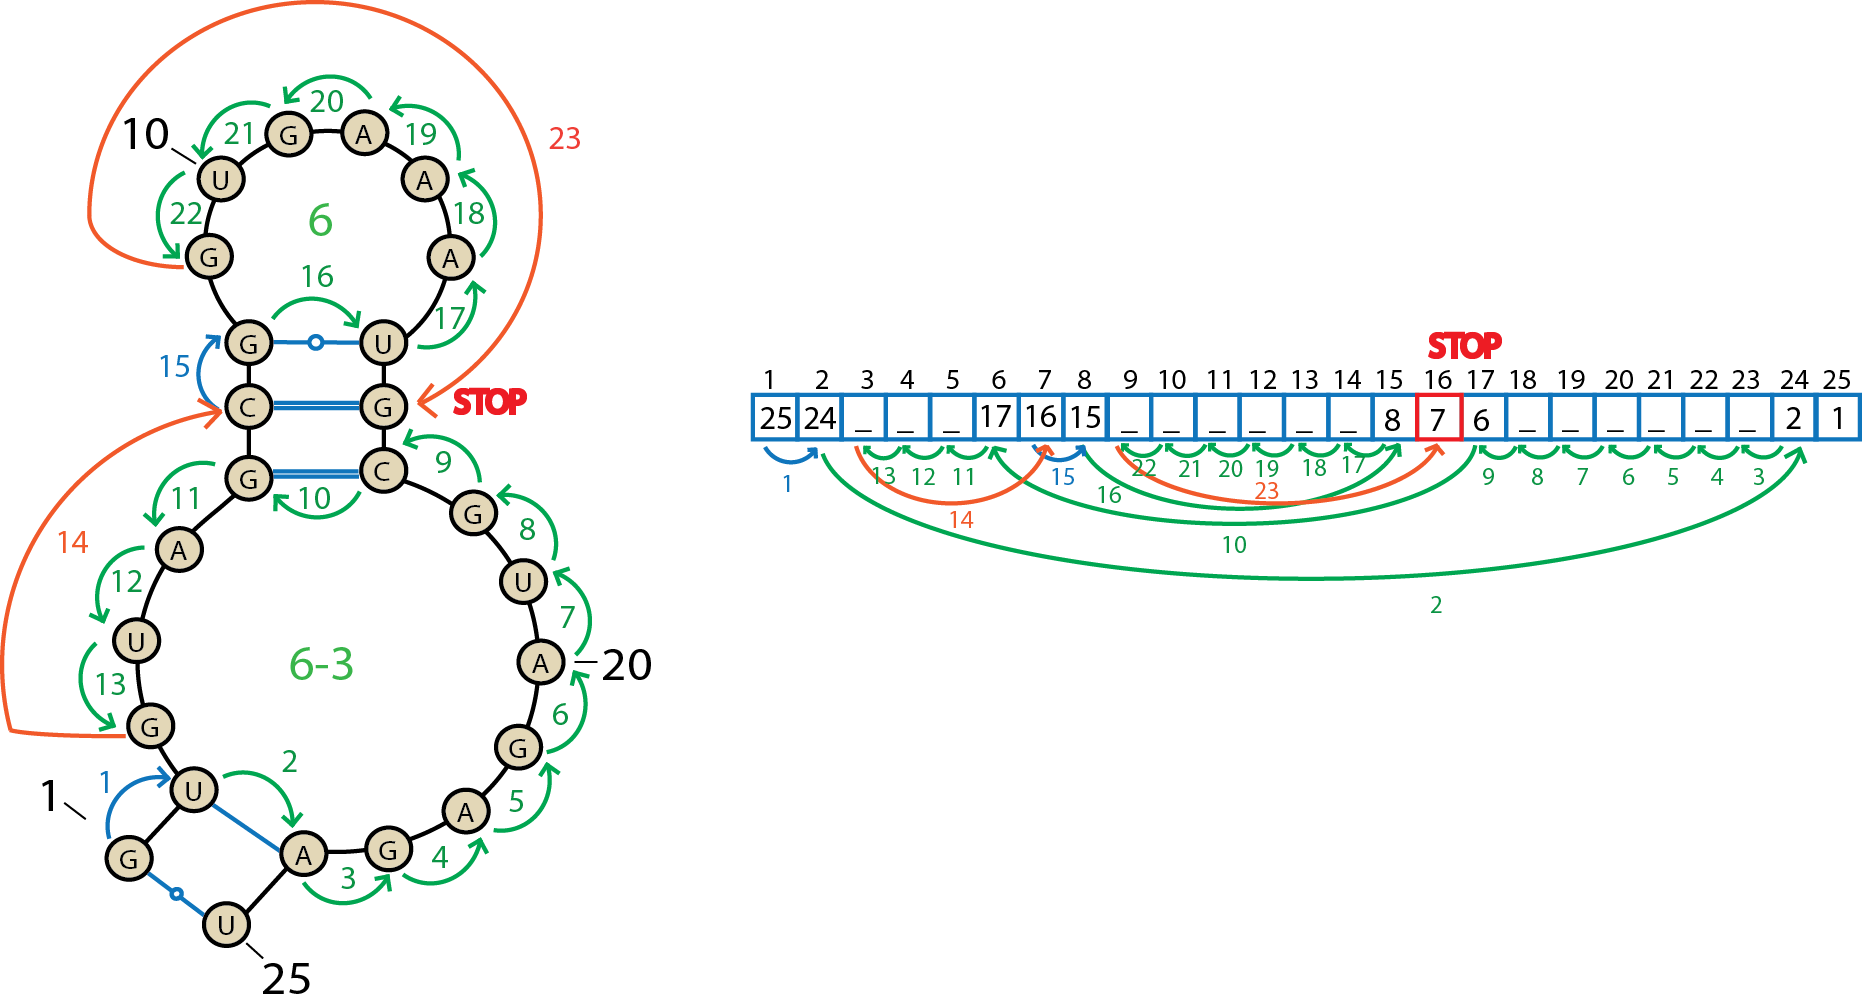
\includegraphics[width =\textwidth]{./pictures/algorithm.png}
\caption{Scheme presenting the steps of the algorithm that finds and classifies the motifs in the RNA structures. The numbers correspond to the step number. Green arrows correspond to the structural motif and blue to the helices. The orange lines denote the jumps after finishing the motif. The STOP sign indicates the position where the algorithm stops.}
\label{MotifsAlgorithm}
\end{figure}

As a result of the single frame analysis the program returns a list of all pairs, motifs and numerical characterization of all nucleotides. Every nucleotide is parametrized with the number of created hydrogen bonds and the description of its partner:

\begin{verbatim}
G538 , 538 , 3-C513A539:1 , 2-C513:2 , 3-C513:7
\end{verbatim}

First the type of the nucleobase with its PDB id, nex the PDB id one more time, and lists of pairs the nucleotide created during the trajectory. Description of the configuration starts with the number of hydrogen bonds, than the nucleobase and PDB ID. There can be more than one nucleotide listed - what indicated the triplex. The number after a semicolon is the number of frames this pair or triplex were present.

\newpage
\section{Trajectory analysis}
If the case of a trajectory in which multiple RNA conformations have to be analyzed and classified, every frame is characterized in detail as previously described. The main output of the program is a set of \texttt{.csv} files listing all the pairs and motifs: helices, triplexes, pseudo-knots etc. and the number of the frames in which the considered structure was present, its topology and participating nucleotides. A detailed description of all the output files can be found in Section~\ref{OutputFiles}.

\subsection{Clustering}
To recognize and characterize the dynamics of the secondary structure of the RNA molecule, we have to cluster the detected secondary structure motifs. Clustering is parameterized with two user-defined parameters: \\
\begin{itemize}
\item \texttt{time\_cutoff} that defines the minimal percentage of frames in which the motif has to be present in order to be classified.
\item \texttt{margin} that defines the minimal percentage of similarities between the two motifs to belong to the common cluster. 
\end{itemize}

The first step is to remove rare motifs (leaving only the significant ones) through filtering them according to the number of frames the motif appeared in. Below one can find an exemplary list of motifs after removing rare motifs:

\begin{figure}[h!]
\centering
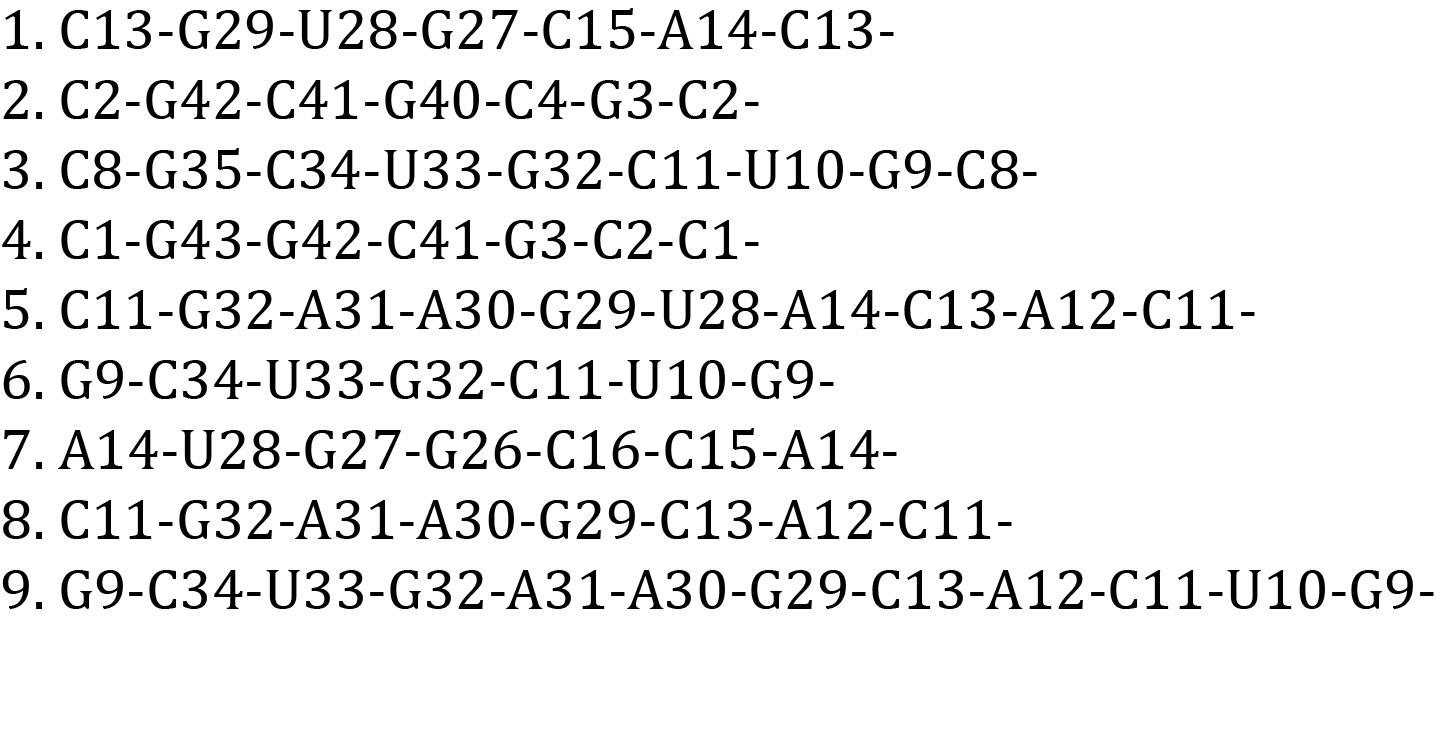
\includegraphics[scale=1]{./pictures/cluster_motif_step1.png}
\caption{First step of clustering.}
\label{MotifsClusteringStep1}
\end{figure}

Next, the motifs distance matrix is computed. The distance between motifs is the number of their common nucleotides. The order of the nucleotides is not taken into account:
\begin{figure}[h!]
\centering
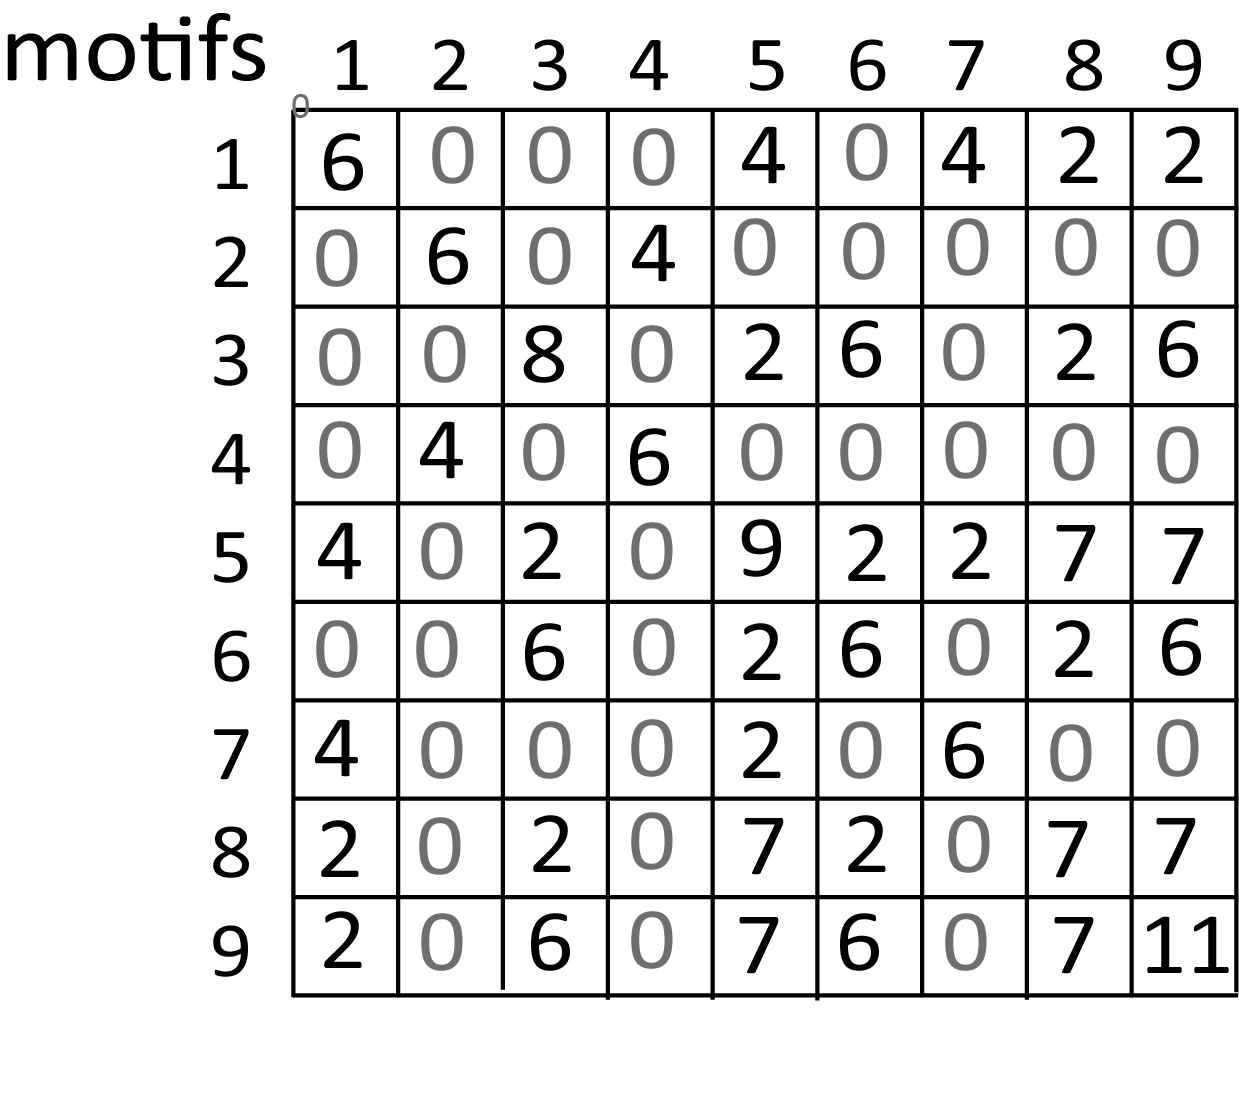
\includegraphics[scale=0.6]{./pictures/cluster_motif_step2.png}
\caption{Exemplary motif distance matrix.}
\label{MotifsClusteringStep2}
\end{figure}

\newpage
Then, the partners for all motifs are denoted. The partner has to satisfy the distance requirement expressed by the equation shown below:
\begin{figure}[h!]
\centering
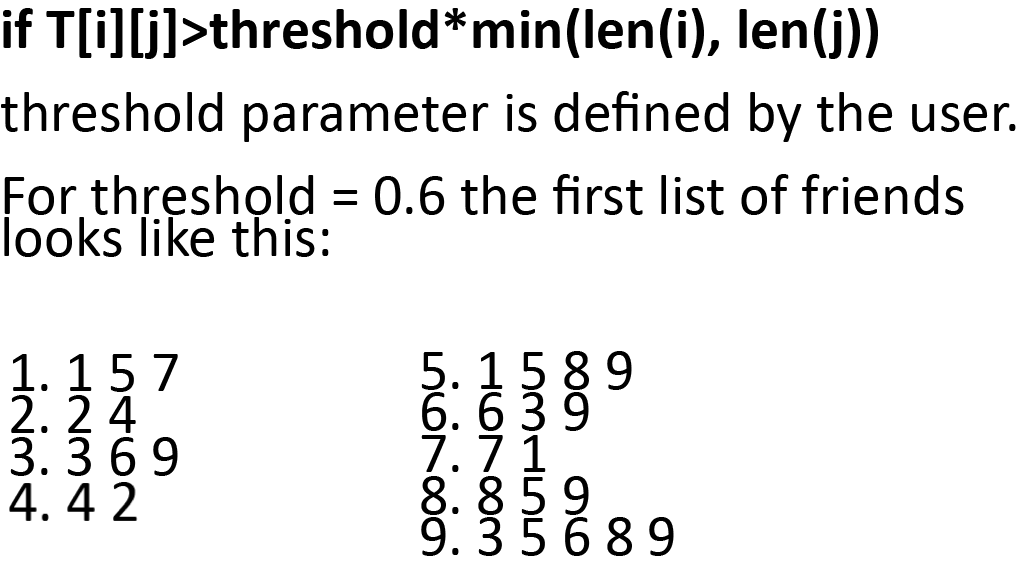
\includegraphics[scale=1]{./pictures/cluster_motif_step3.png}
\label{MotifsClusteringStep3}
\caption{Equation with distance requirement that motifs has to satisfy to be partners.}
\end{figure}

Next, the motif with the longest list of partners is incorporated as the first one to the first cluster number zero. The motifs used in the first cluster have to be crossed out from the rest. Then the second longer is chosen, the picked motifs are crossed out and so on.  

\begin{figure}[h!]
\centering
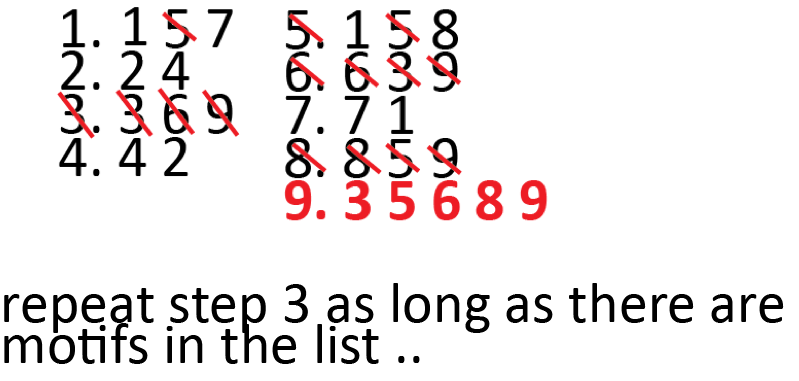
\includegraphics[scale=1]{./pictures/cluster_motif_step4.png}
\label{MotifsClusteringStep4}
\caption{Removal of partners from a list of motifs}
\end{figure}

\begin{figure}[h!]
\centering
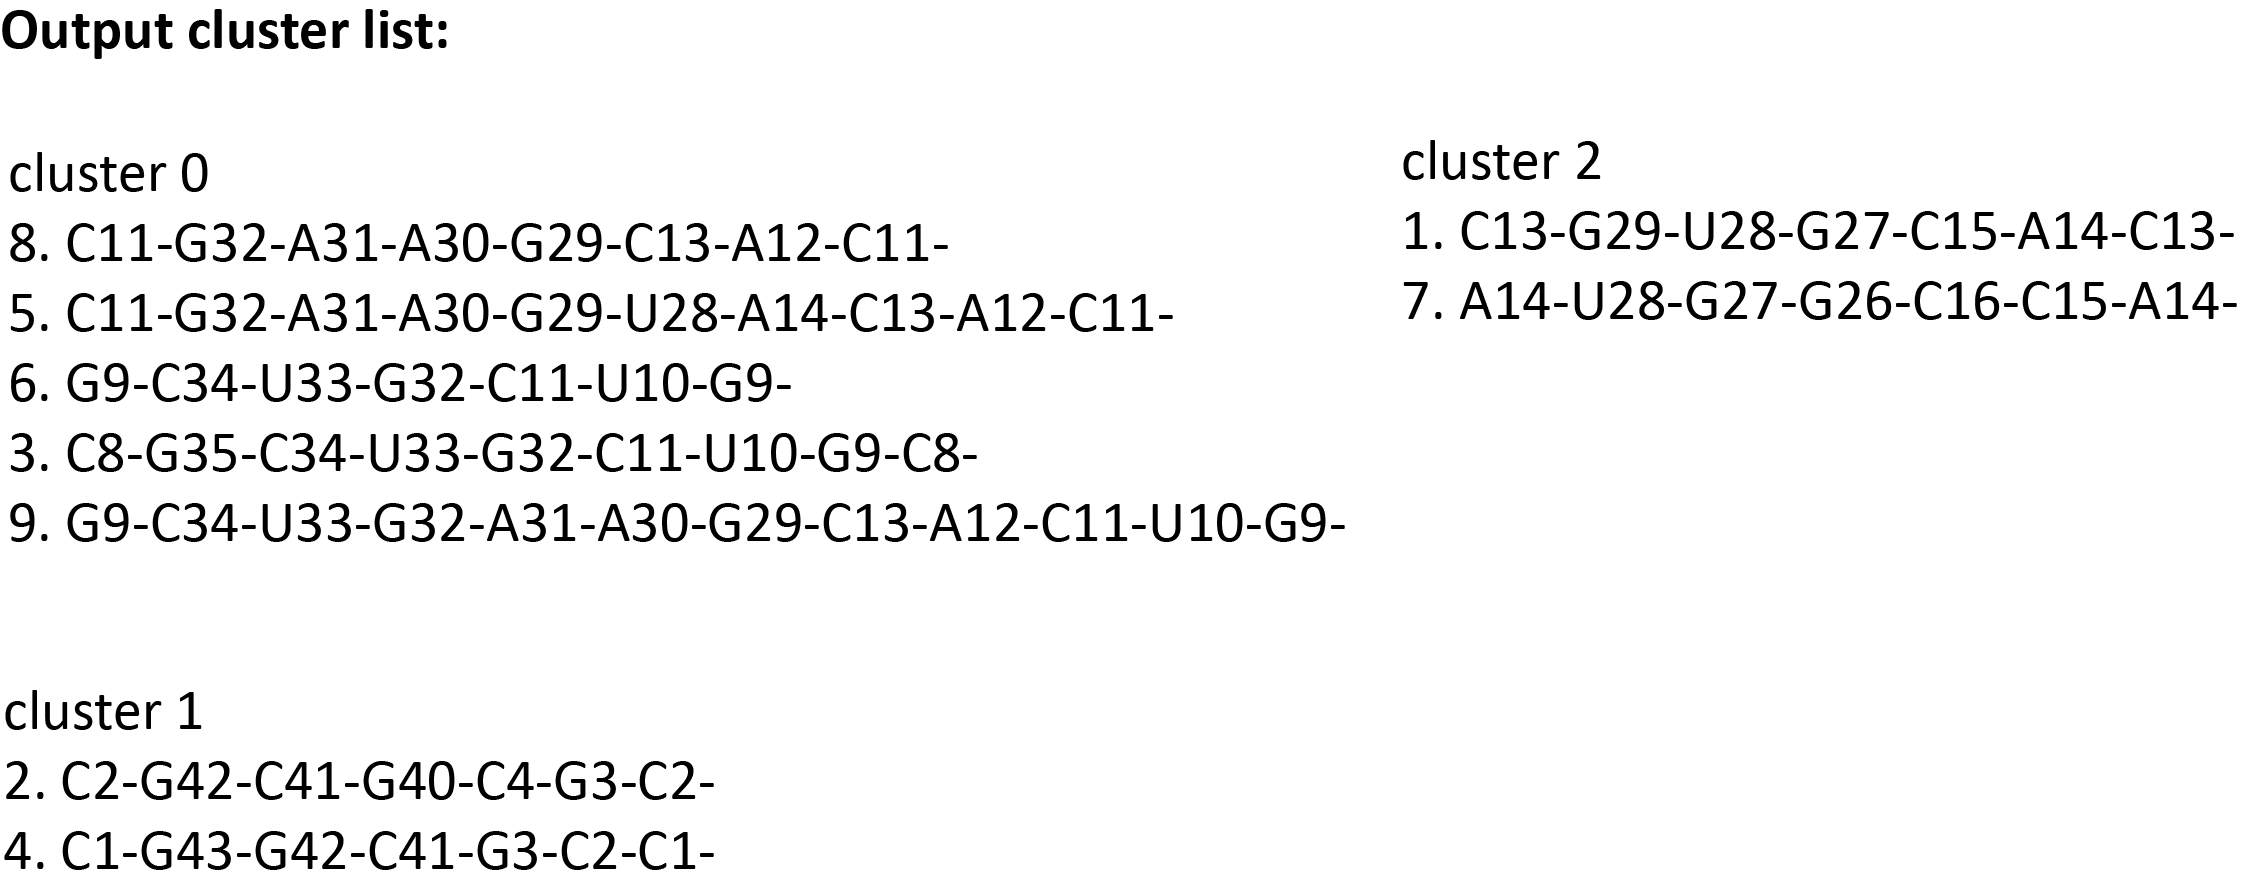
\includegraphics[scale=1]{./pictures/cluster_motif_step5.png}
\label{MotifsClusteringStep5}
\caption{Result of the clusterization process.}
\end{figure}

Additionally, the average clusters are returned. The list consists of the longest motif for every cluster and the two vectors of float values describing every nucleotide participating in the representative motif. The float vectors represent the average number of hydrogen bonds created by a nucleotide in both WC-WC pairs and other interactions. We hope to show the average secondary structure of the molecule within the tertiary structure description. While analyzing the whole output generated by the script, one can understand the complex description of the RNA structure in the dynamics.

% Visualization - odnosnik do VMD gdzies sie powinien pojawic.



\section{Visualization}\label{Visualization}
MINT enables many different ways of data visualization. The user can display a colored input PDB structure according to several parameters (motifs, secondary and tertiary contacts, electrostatic, VDW energies) both in the \texttt{Single} and \texttt{Trajectory} modes. The same parameters are colored on the secondary structure. 

For visualization it is preferable to install the following programs:
\begin{itemize}
\item {\tt VMD}\cite{Humphrey1996}, or {\tt Chimera}~\cite{Pettersen2004} for tertiary structure visualization.
\item {\tt RNAMovies} for secondary structure trajectory visualization (\url{http://bibiserv.techfak.uni-bielefeld.de/rnamovies/}).
\end{itemize}

\subsection{Representing motifs on the tertiary structure} 
\label{VMD}
These feature works through creating representations of the regions of the nucleic acid molecule in the input PDB file using the VMD program \cite{Humphrey1996}. In the \texttt{VMD} one can represent fragments of molecule using different representations and color, all can be managed from \texttt{Graphical Representations} menu (\texttt{Graphics > Representations}). The \texttt{vmd\_tcl} script loads the structure and creates \texttt{Reps} for every motif and helix in the structure what results with a view of the three-dimensional molecule colored accordingly to the detected structural components:

\begin{itemize}
\item helices: yellow (vmd color code:4)
\item pseudo-knots: tan (vmd color code:5)
\item triplexes: silver (vmd color code:6)
\item loops: green (vmd color code:7)
\end{itemize}

If the \texttt{VMD} program is in your PATH you can turn on the \texttt{vmd} parameter and it will launch automatically. Otherwise, you can do it manually by going into your MINT inputs/outputs catalog and typing in the terminal:

\texttt{your\_vmd\_location$\backslash$vmd -e vmd\_run.tcl }

\begin{figure}[h!]
\centering
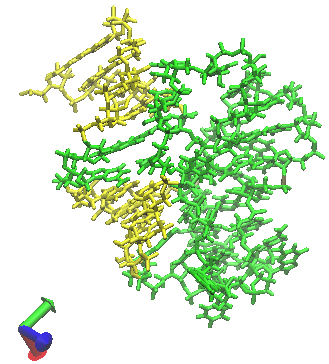
\includegraphics[scale=0.8]{./pictures/motifs_vmd.png}
\caption{Result of running the exemplary structure \texttt{vmd\_run.tcl} script in the VMD program after changing display into \texttt{Orthographic} and changing the background color.}
\end{figure}

\subsection{Representing hydrogen bonding and stacking on the tertiary structure} The program produces several PDB files with the B-factor column replaced with the values of:
\begin{itemize}
\item \texttt{\_2D.pdb} -- the number of hydrogen bonds in the WC pairs created by the given nucleotide.
\item \texttt{\_3D.pdb} -- the number of hydrogen bonds in the non-WC pairs created by the given nucleotide.
\item \texttt{\_coulomb.pdb} -- the value of the Coulomb energy for a given nucleotide  (the sum of all interactions the nucleotide is involved in).
\item \texttt{\_VDW.pdb} -- the value of the Van der Waals energy for a given nucleotide (the sum of all interactions the nucleotide is involved in).
\item \texttt{\_stacking\_sum.pdb} -- the sum of Van der Waals and Coulomb energies. 
\end{itemize}

In the case of trajectory these PDB files contain the average values for the analyzed trajectory. Here, we describe a short manual on how to visualize the computed data using VMD or Chimera.

\paragraph{VMD}
\texttt{VMD} is a powerful tool that has a complete user guide and tutorial that can be found on the VMDs home website (\url{http://www.ks.uiuc.edu/Research/vmd/}).
The user has to open the \texttt{VMD} program and load one of the PDB files, through choosing the \texttt{New Molecule} from the \texttt{File} drop-down menu. As it is shown below:

\begin{figure}[h!]
\centering
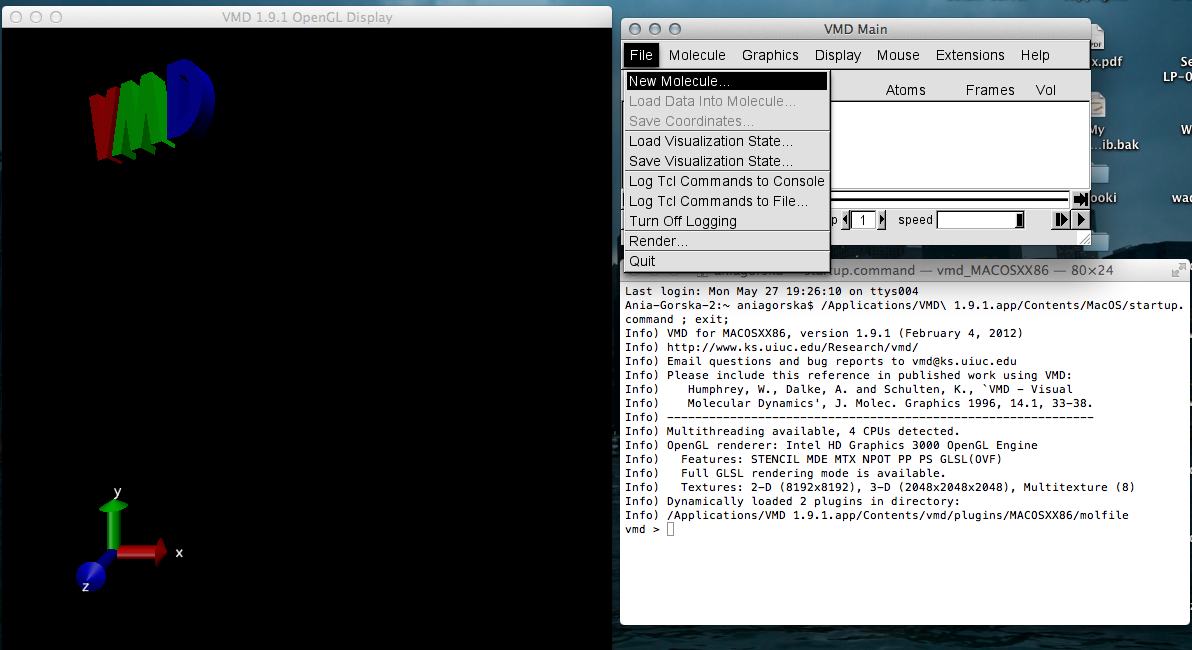
\includegraphics[scale=0.4]{./pictures/vmd1.png}
\caption{Loading a pdb file into the VMD program.}
\end{figure}

Next, one has to \texttt{Browse} and \texttt{Load} a desired PDB file:
\begin{figure}[h!]
\centering
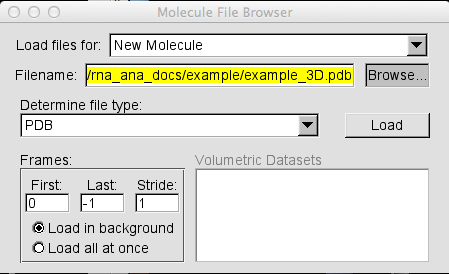
\includegraphics[scale=0.4]{./pictures/vmd2.png}
\caption{Loading a pdb file into VMD program.}
\end{figure}
\newpage
Having the loaded structure, one needs to open the \texttt{Representations} window from the \texttt{Graphics} drop-down menu:
\begin{figure}[h!]
\centering
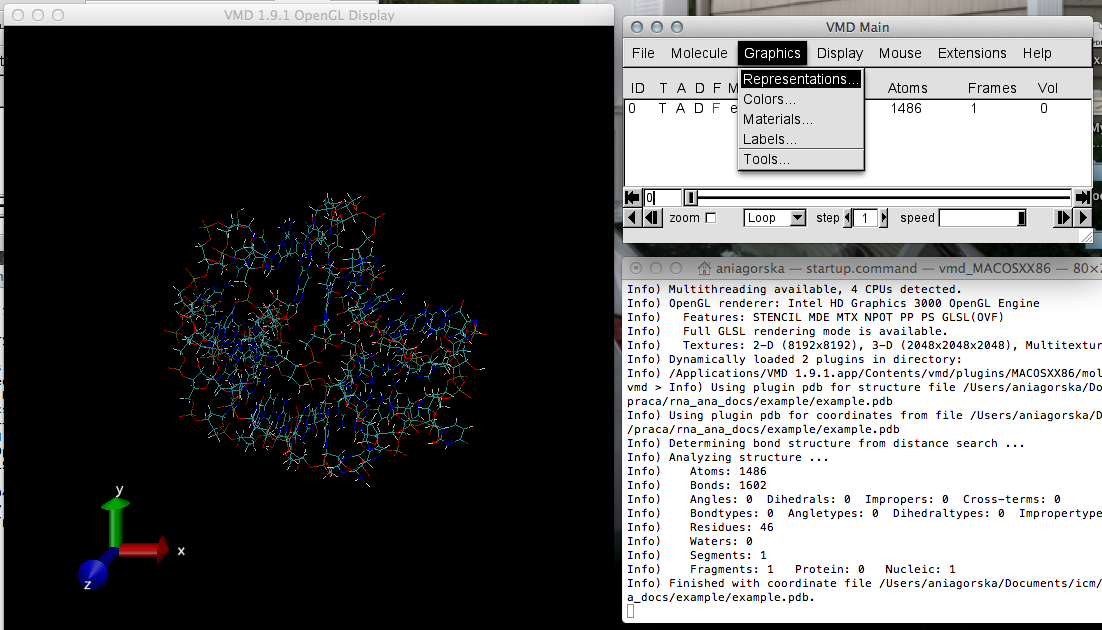
\includegraphics[scale=0.4]{./pictures/vmd3.png}
\caption{Opening the representation window in VMD.}
\end{figure}

The \texttt{Representations} menu allows one to create multiple different representations. To color the structure by the B-factor column from the PDB file, we propose to change the \texttt{Drawing Methods} into the \texttt{New Cartoon} and the \texttt{Coloring Method} into the \texttt{Beta}:

\begin{figure} [h!]
\begin{center}
\subfigure[]{
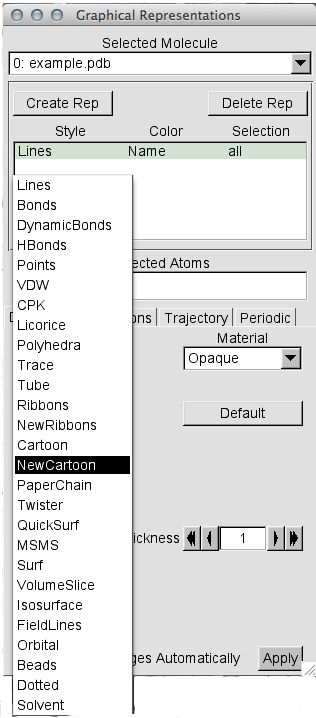
\includegraphics[scale=0.325]{pictures/vmd4.png}}
\subfigure[]{
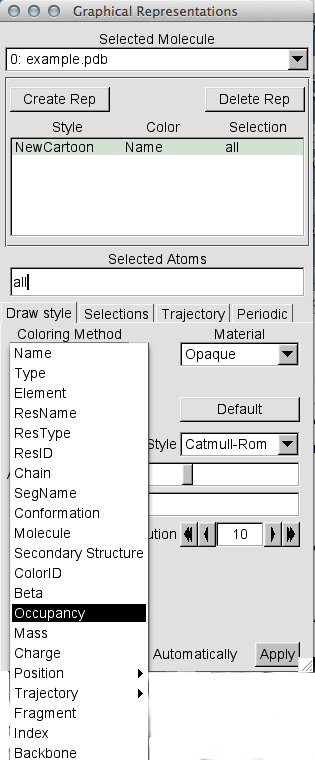
\includegraphics[scale=0.3]{pictures/vmd5.png}}
\end{center}
\caption{Choosing \texttt{Drawing} and \texttt{Color Methods} in the VMD program.}
\end{figure} 

\newpage
Then the color scale can be altered through \texttt{Graphics} $>$ \texttt{Color} $>$ \texttt{Color Scale}:

\begin{figure}[h!]
\centering
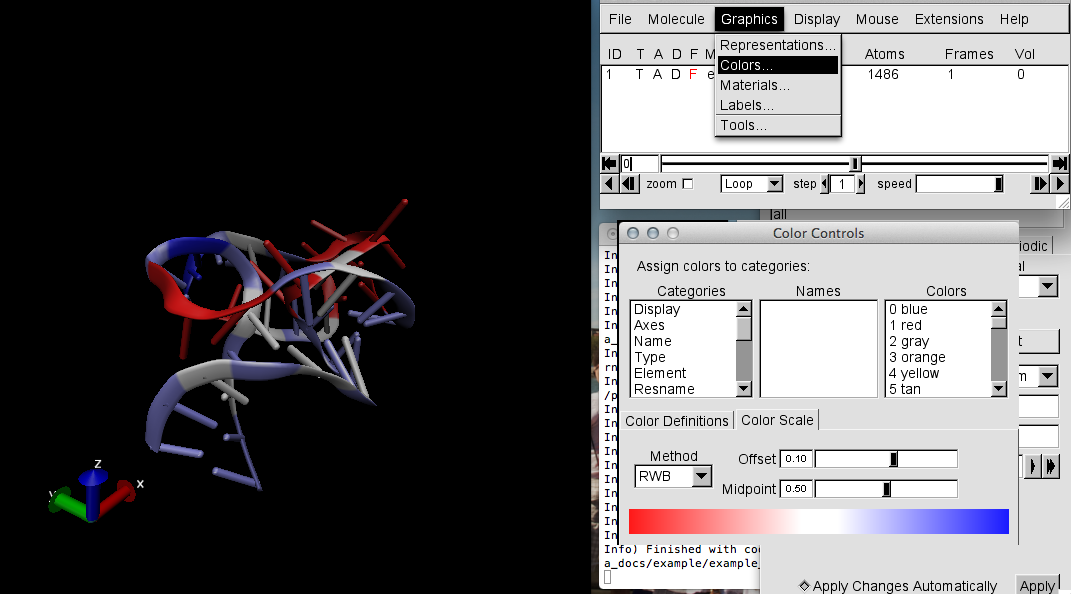
\includegraphics[scale=0.4]{./pictures/vmd6.png}
\caption{Changing the colors scale.}
\end{figure}

If you proceed in the same way with more than one PDB structure you can use the \texttt{Move} tool (\texttt{Mouse} $>$ \texttt{Move} $>$ \texttt{Molecule}) and view the colored structures at the same time as it is presented in Figure \ref{3Ddifferent}.

\begin{figure}[h!]
\centering
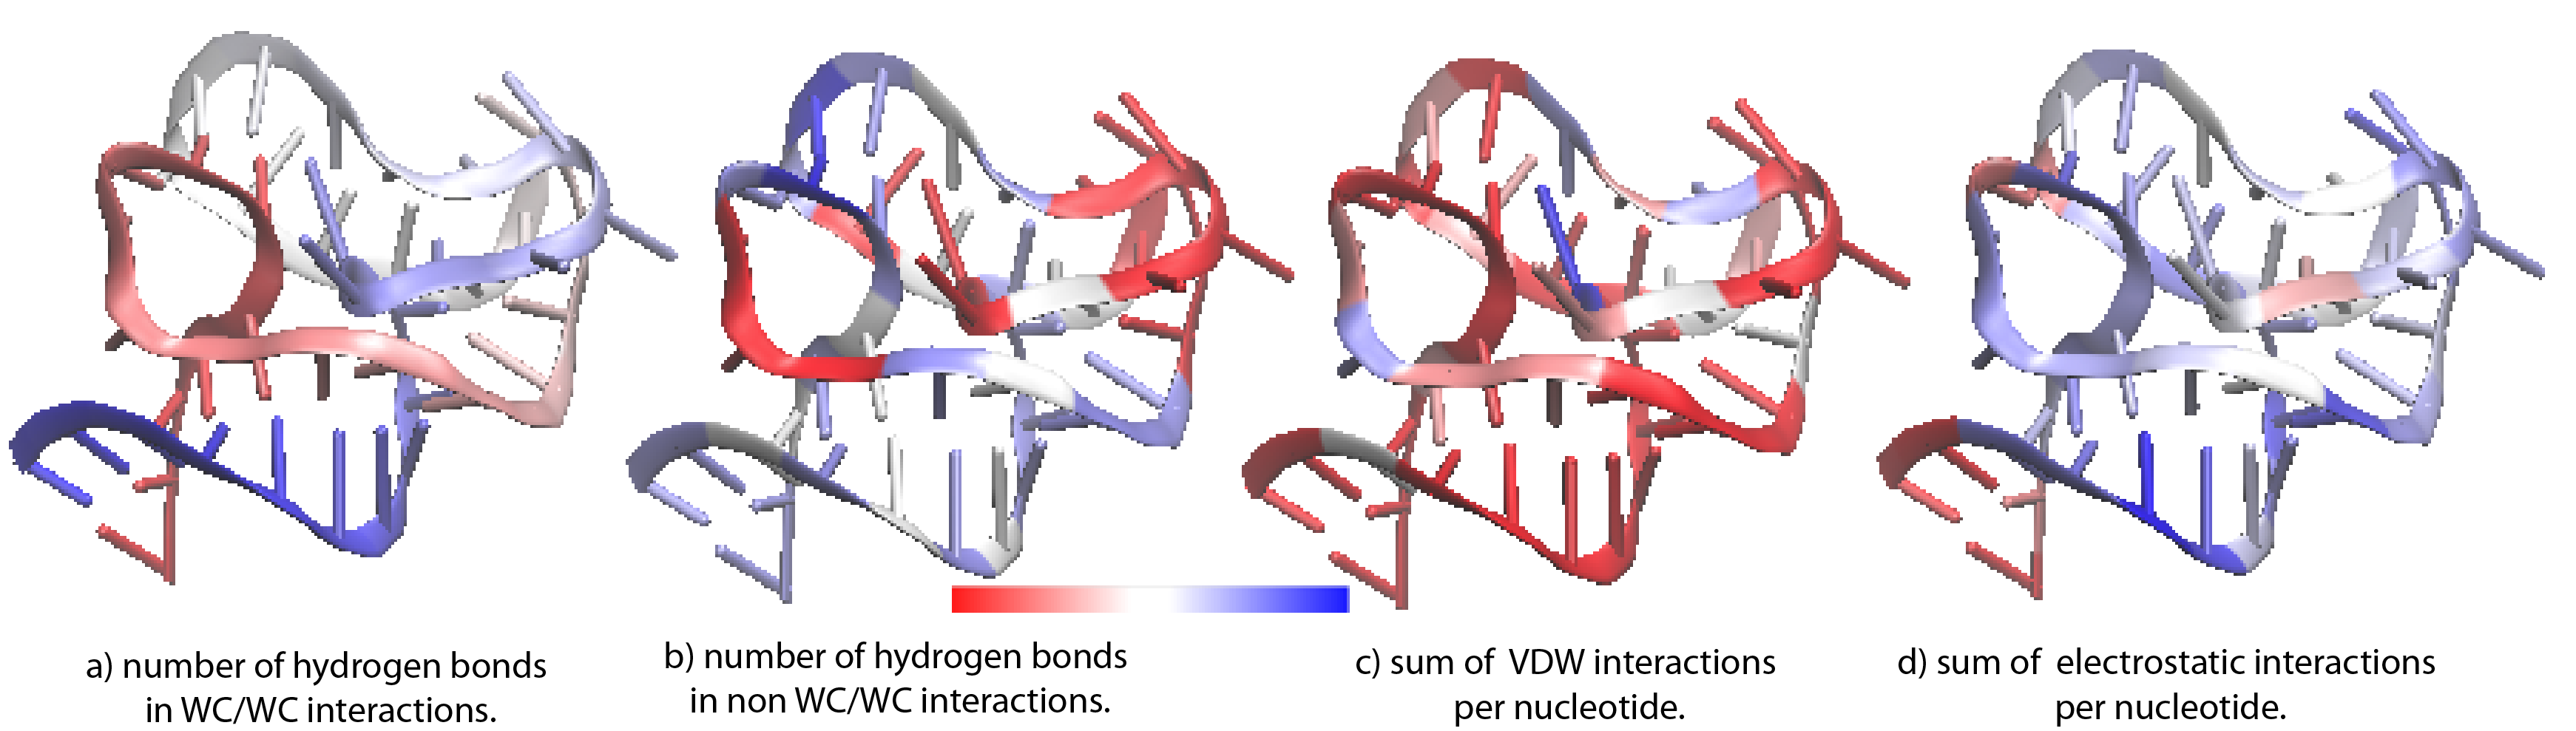
\includegraphics[scale=0.65]{./pictures/3D_different.png}
\caption{Exemplary pictures created with the use of the VMD program and the PDB files created by MINT.}
\label{3Ddifferent}
\end{figure}

\paragraph{Chimera}
High quality 3D visualizations can be done also with {\tt Chimera} software (details about how to use the program can be found at (\url{https://www.cgl.ucsf.edu/chimera/}). The user has to open {\tt Chimera} and load one of the PDB files. Than choose from \texttt{Tools} menu the \texttt{Depiction} section and click on the \texttt{Render by Attribute}. As it is shown in Figure~\ref{chimera1}.

\begin{figure}[h!]
\centering
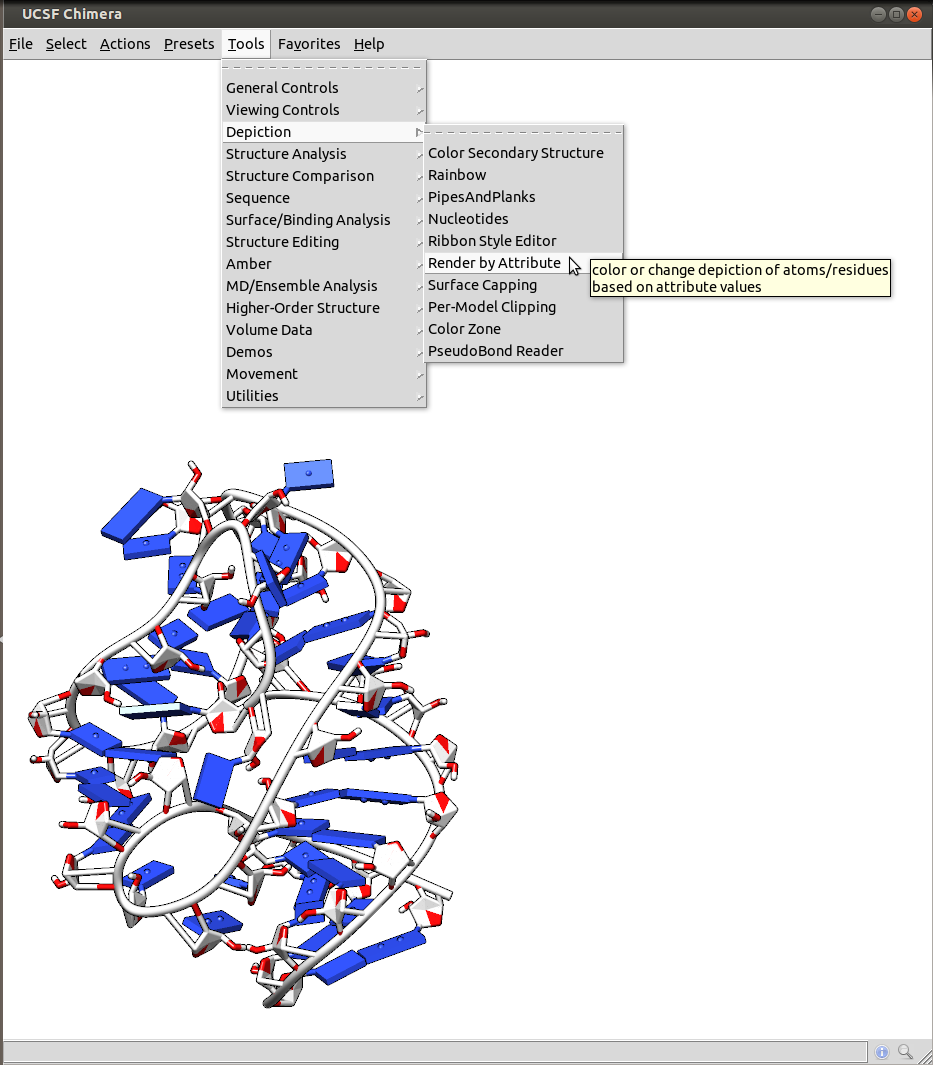
\includegraphics[scale=0.3]{./pictures/chimera1.png}
\caption{Render by attribute menu in the Chimera.}
\label{chimera1}
\end{figure}

In the opened window (Figure~\ref{chimera22}) the user chooses attributes of \texttt{residues} instead of default \texttt{atoms}. The \texttt{Attribute:} should be changed to \texttt{average -> bfactor}. Than colors scale and palette can be chosen and the color key can be created. Two exemplary pictures rendered in {\tt Chimera} are presented in Figure~\ref{chimera-pictures}.
\begin{figure}[!h]
\centering
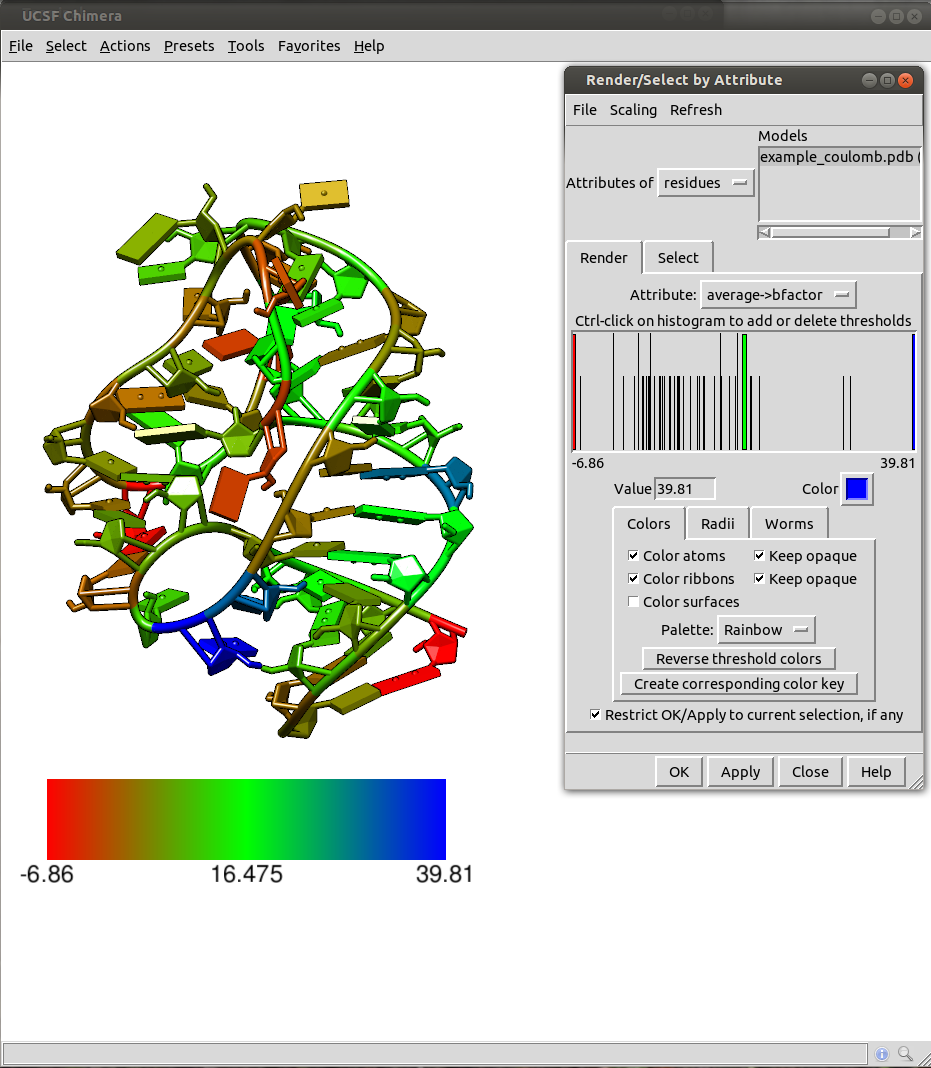
\includegraphics[scale=0.3]{./pictures/chimera2.png}
\caption{Rendering structure by attribute in the Chimera program using the PDB file created by MINT.}
\label{chimera22}
\end{figure}


\begin{figure}[!h]
%\centering
\hspace*{\fill}%
\subfigure[Average number of WC hydrogen bonds per nucleotide]{
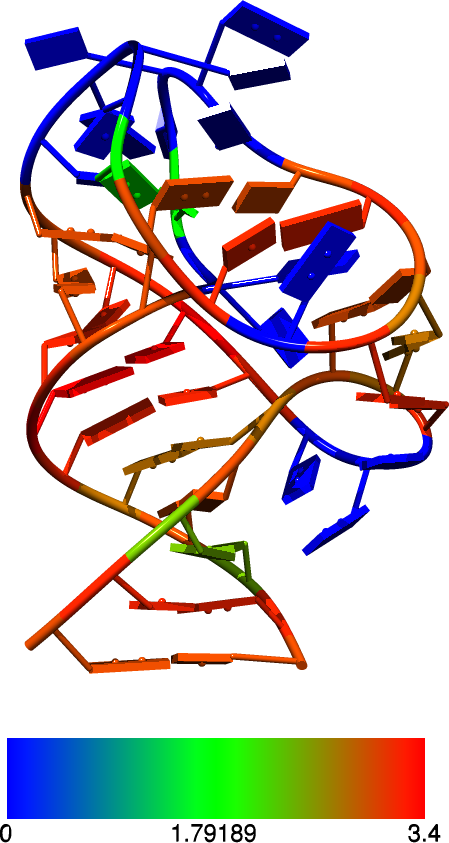
\includegraphics[scale=0.3]{./pictures/chimera-2D.png}}\hfill%
\subfigure[Average energy (in kcal/mol) of stacking interaction per nucleotide]{
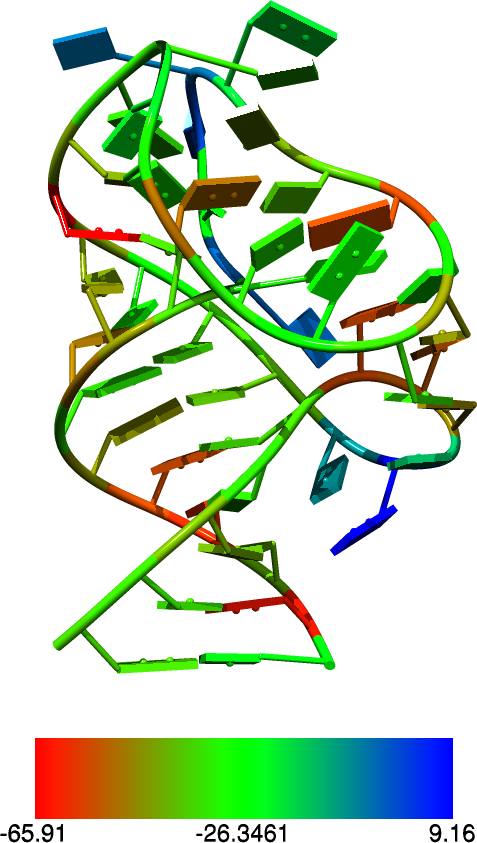
\includegraphics[scale=0.3]{./pictures/chimera-stacking.png}}
\hspace*{\fill}%
\caption{Exemplary pictures created with the use of the Chimera program and the PDB files created by MINT.}
\label{chimera-pictures}
\end{figure}


\newpage
\newpage
\subsection{Secondary structure trajectory representation} 
An analysed trajectory can be visualized in the secondary structure representation with the RNAMovies \cite{Evers1999} program. The MINT returns the \texttt{RNAStructML.xml} file containing the trajectory of the secondary structure. For every frame the dot-bracket representation is written into the .xml file. This allows to produce the movie of the secondary structure trajectory. 

The RNAMovies \cite{Evers1999}  java .jar file can be downloaded from its home page: \url{http://bibiserv.techfak.uni-bielefeld.de/rnamovies/}. Here we present a short tutorial on how to open a .xml file and view the trajectory.

First, one has to open the RNAMovies and choose the \texttt{Import} option from the \texttt{File} drop-down menu. 
\begin{figure}[h!]
\centering
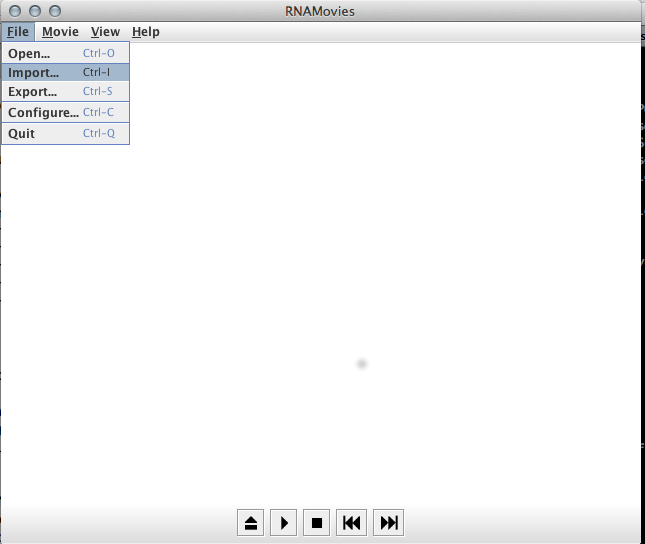
\includegraphics[scale=0.4]{./pictures/RNAmovies_1.png}
\end{figure}
\newpage
Find a proper .xml file in your disk, and click \texttt{Open}:
\begin{figure}[h!]
\centering
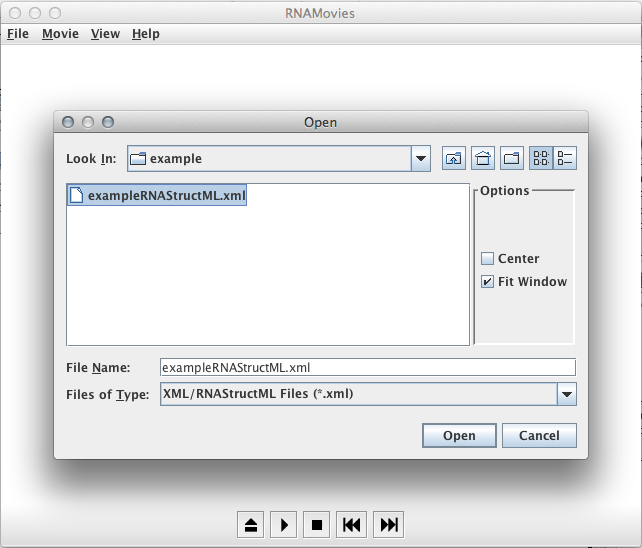
\includegraphics[scale=0.4]{./pictures/RNAmovies_2.png}
\end{figure}

One can navigate the trajectory using the arrows in the bottom of the window. If you want to loop the trajectory or change the pace go to the \texttt{File} $>$ \texttt{Configure} menu: 
\begin{figure}[h!]
\centering
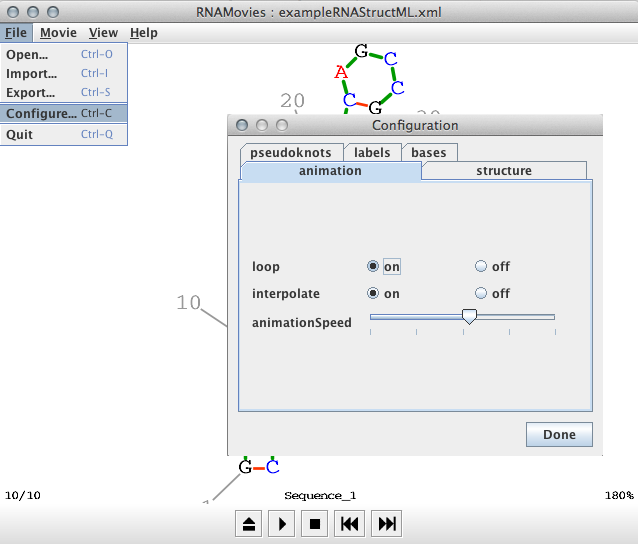
\includegraphics[scale=0.4]{./pictures/RNAmovies_3.png}
\end{figure}
\newpage
The animated trajectory can be written into the .gif file  (\texttt{File} $>$ \texttt{Export}).

\subsection{Correlations}\label{CorrelationsParagraph}
In the \texttt{MINT} directory the user can find an additional python script \texttt{CORRELATIONS.py} computing \texttt{phi coefficient} for every pair of nucleotides in the structure. The \texttt{phi coefficient} is computed using the equation \cite{Everitt1977}:
\begin{center}
\begin{large}
$ \phi = \frac{n_{11}n_{00}}{\sqrt{n_{\bullet1}n_{\bullet0} n_{0\bullet}n_{1\bullet}}}$
\end{large}
\end{center}

where:
\begin{itemize}
\item $n_{11}$ is a number of frames when both nucleotides are creating WC pair.
\item $n_{00}$ is a number of frames when none of the nucleotides is creating WC pair.
\item $n_{01}$ is a number of frames when first of the nucleotides is creating WC pair and the second nucleotide is not, analogously $n_{10}$ is the number of frames when first nucleotide is paired and second is free.
\end{itemize}

and:
\begin{itemize}
\item $n_{\bullet1} = n_{11}+n_{01}$
\item $n_{1\bullet} = n_{11}+n_{10}$
\item $n_{\bullet0} = n_{00}+n_{10}$
\item $n_{0\bullet} = n_{00}+n_{01}$
\end{itemize}

\begin{figure}[h!]
\label{coefficient}
\centering
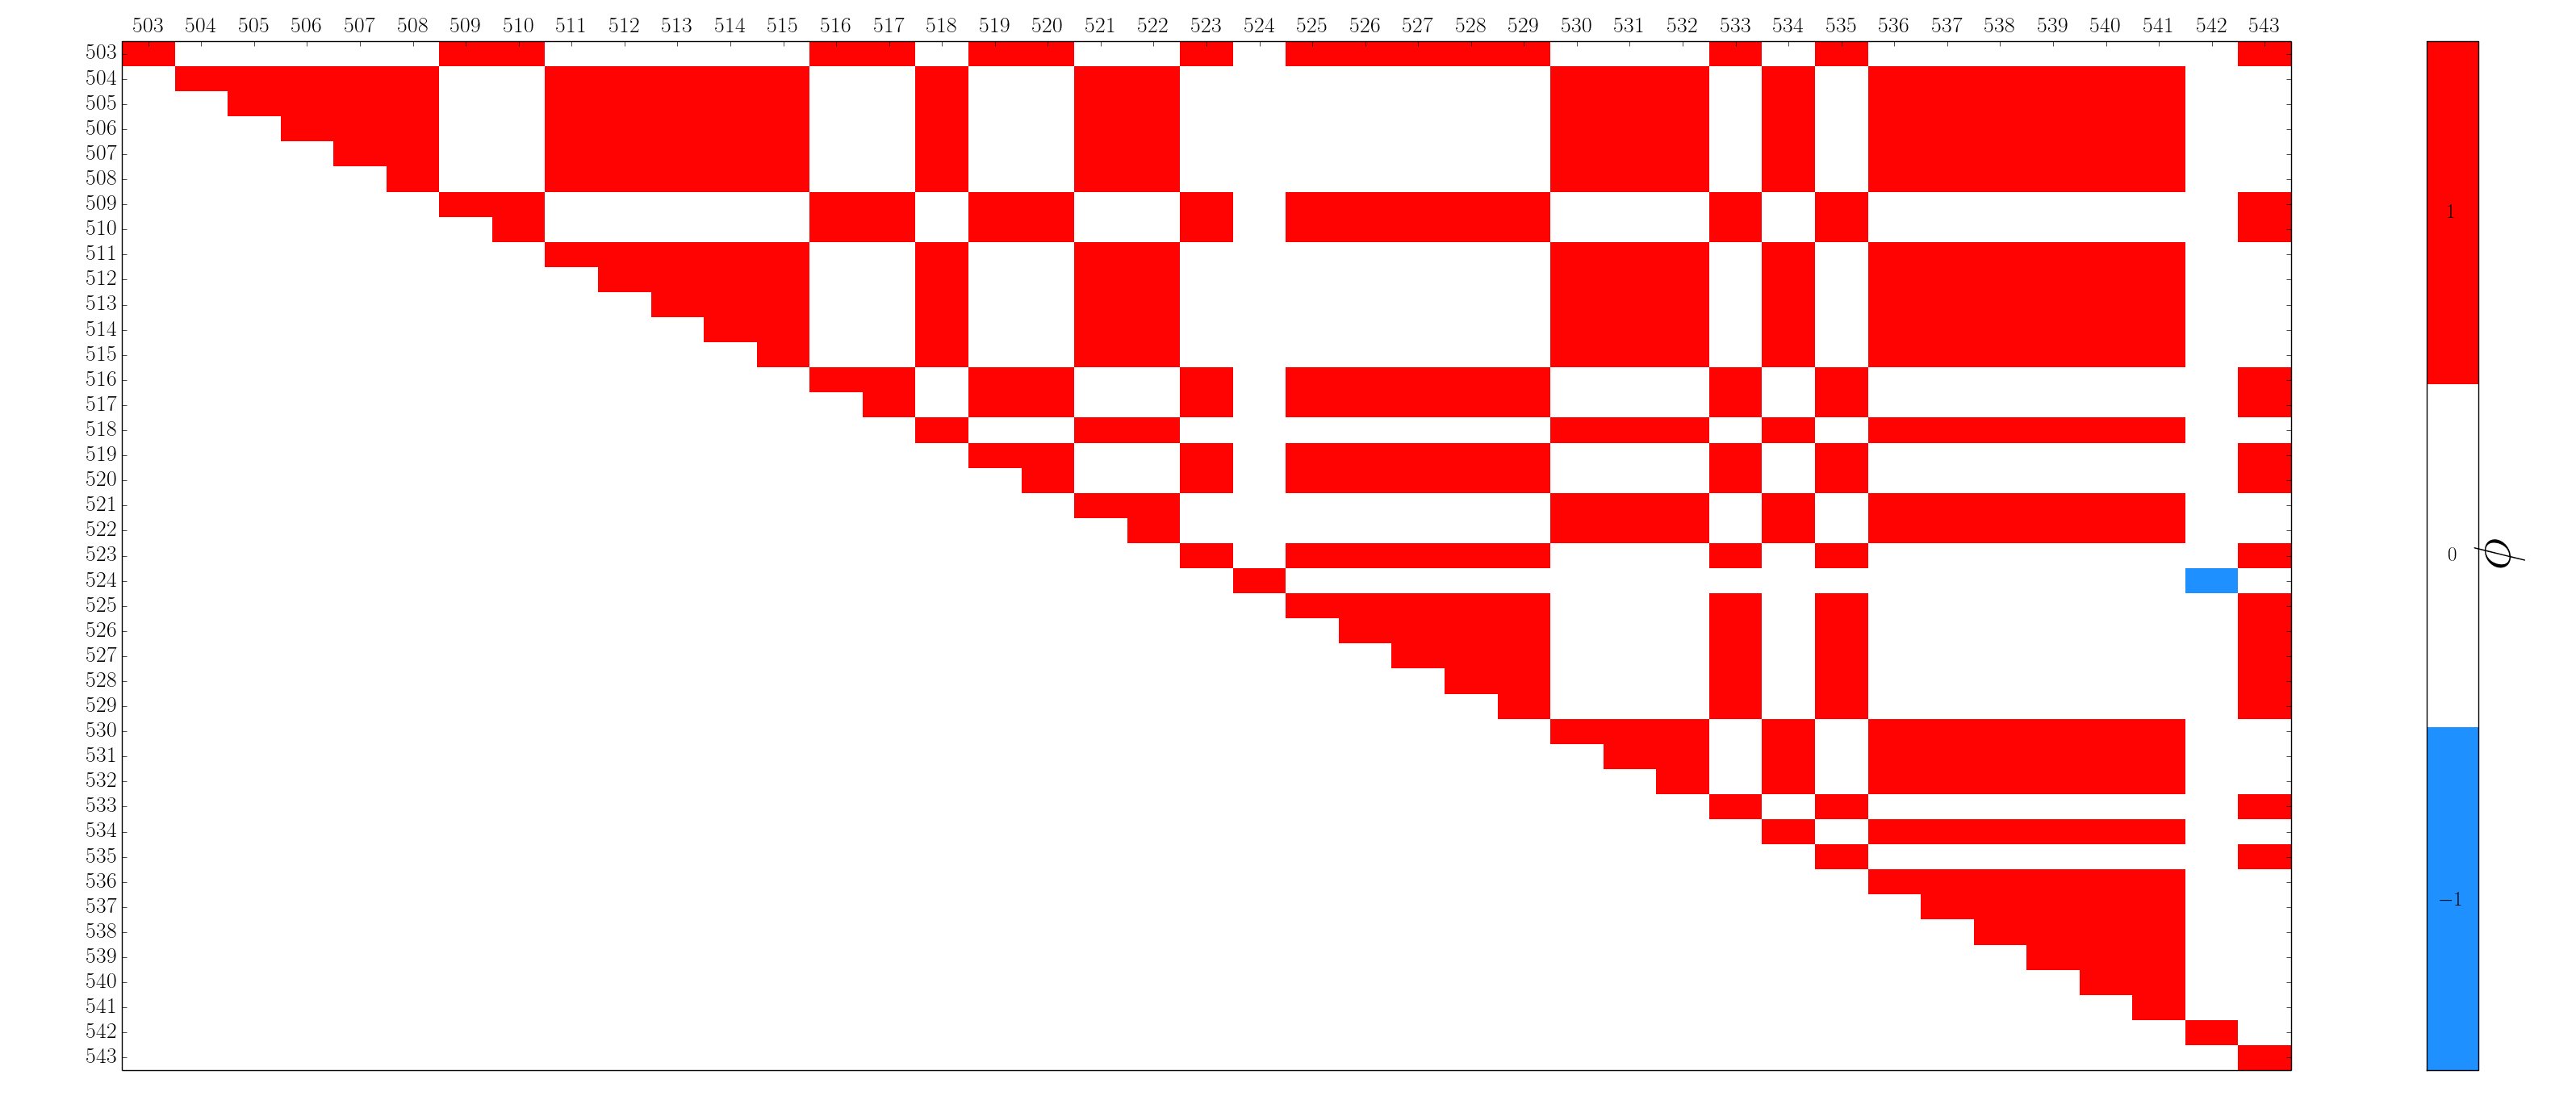
\includegraphics[scale=0.4]{./pictures/correlation_matrix.png}
\caption{Heap map of \texttt{phi coefficient} for the the same exemplary molecule as shown before, and for discussed trajectory. These map was calculated with 0.4 \texttt{cutoff}.}
\end{figure}

\texttt{Phi coefficient} takes values between -1 and 1. It is believed that when coefficient value is close to 0 the correlation is not reliable. In the heat map, all values larger then \texttt{cutoff} will be marked red, all lower than \texttt{-1*cutoff} are marked blue. The rest will remain white. The level of \texttt{cutoff} is defined by the user.

The script produces a matrix that is both written into the text file and printed in the form of the heat map. Figure \ref{coefficient} presents heat map of \texttt{phi coefficient} for the previously discussed exemplary RNA molecule and its 10 frame-long molecular dynamics.

\texttt{CORRELATIONS.py} script uses as an input: the \texttt{MINT} output \texttt{pairs\_in\_time.csv} type, cutoff and list of numbers of nucleotides you want to compute the coefficient for.


To compute the phi coefficient for all nucleotides type:
\begin{verbatim}
python CORRELATIONS.py filename_pairs_in_time.csv 0.4
\end{verbatim}
where \texttt{filename} is name of your csv file and \texttt{0.4} is an example of the \texttt{cutoff} for these calculations.
To compute the phi coefficient only for specified nucleotides type:\\

\begin{verbatim}
python CORRELATIONS.py filename_pairs_in_time.csv 0.4 "[(1210,1220),(985,995)]" 
\end{verbatim}

The list of nucleotides has to be specified in the square brackets and quotation marks. Inside round brackets the ranges of nucleotides must be specified. 

Heat map is only printed for the half of the matrix, another half would be identical. All of the nucleotides are correlated with themselves - the diagonal is coloured in red. All of the nucleotides creating WC pairs with each other are also positively correlated. The neighbouring pairs that work together will also be visible as correlated in all to all manner. The negative correlation suggests that there are pairs that opens when another one closes.


\section{Appendices}
\begin{appendices}
\subsection{Adding hydrogens to a PDB structure}
The hydrogen bond definition used in {\tt MINT} requires the hydrogen atom to measure the angle, therefore the input has to be full-atom.

If one analyzes the files from MD simulations, the hydrogen atoms were added to the structure during the preparation of an MD run, according to the atom type definitions in the used force field. Various tools from the MD packages can be used to assign the positions of hydrogens (for example Xleap from AmberTools). 

However, if a structure from the PDB database has to be analyzed and the user does not have experience with MD methods, hydrogen atoms can be added using on-line servers. We have tested a few of them and we can recommend the {\tt Molprobility} service~\cite{Chen2010} (\url{http://molprobity.biochem.duke.edu/}). It works even with the structures as large as the ribosomal subunits in an acceptable time span. What is more, the software can be downloaded from the \url{http://kinemage.biochem.duke.edu/software/reduce.php} website and used offline.

\subsection{Exemplary description file}
Fragment of the \texttt{\_description} file generated during analysis of an \texttt{example.dcd} trajectory.
\begin{scriptsize}
\begin{lstlisting}
Running with parameters: 
cutoff=20.0
file_name=1e8o/1e8o_H.pdb
vmd=1
h_bond_l=4.0
MINT_home=/Users/agorska/Documents/mint
SingleOrTraj=Single
max_memory_GB=1.5
table_charges=/Users/agorska/Documents/mint/data/charges_and_VDW_modified.csv
vdw_cutoff_stacking=0.0
h_bond_atom=donor
list_of_modified_nucs=data/unknown_modified.fa
only_analysis=0
h_bond_angle=140.0
force_field=AMBER
pdb_list=
chains_names=[]
cutoff_stacking=10.5
table_nucleotides=/Users/agorska/Documents/mint/data/nucleotides_modified.csv
margin=0.8
OP_stacking_distance_cutoff=4.5

  50 nucleotides, sequence: 
GDP G G C C G G G C G C G G U G G C G C G C G C C U G U A G U C C C A G C U A C U C G G G A G G C U C 
Nucleotides statistics:
GDP-> 1 UNknown parameters
A  -> 4 known parameters
C  -> 17 known parameters
U  -> 7 known parameters
G  -> 21 known parameters

Stacking pairs
 qn1 n2     Coul     VdW    sum
E|GDP:99 E|G:100 MODIFIED NUCLEOTIDES
E|G:100 E|G:101(6.81, -29.13, -22.32)
E|G:100 E|C:148(0.87, -15.41, -14.54)
E|G:101 E|C:102(-5.15, -27.25, -32.4)
E|G:101 E|U:147(2.39, -8.82, -6.43)
E|G:101 E|C:148(1.21, -0.83, 0.38)
E|C:102 E|C:103(2.45, -16.48, -14.04)
E|C:102 E|G:104(0.29, -0.01, 0.27)
E|C:102 E|G:127(-0.46, -0.17, -0.63)
E|C:102 E|C:146(7.14, -3.61, 3.52)
E|C:102 E|U:147(0.04, -0.48, -0.44)
E|C:103 E|G:104(0.43, -0.05, 0.38)
E|C:103 E|U:125(0.89, -0.04, 0.86)
E|C:103 E|G:127(0.58, -0.23, 0.36)
E|C:103 E|U:128(-0.18, -16.47, -16.64)
E|C:103 E|G:145(0.78, -12.04, -11.26)
E|C:103 E|C:146(-0.29, -0.68, -0.97)
E|G:104 E|G:105(4.39, -28.74, -24.36)
E|G:104 E|G:124(10.25, -47.13, -36.88)
E|G:104 E|U:125(1.61, -1.07, 0.55)
E|G:104 E|G:127(0.33, -0.07, 0.26)
E|G:104 E|U:128(0.26, -0.06, 0.2)
E|G:105 E|G:106(4.16, -33.32, -29.16)
E|G:105 E|U:123(-0.56, -18.01, -18.57)
E|G:105 E|G:124(2.04, -1.12, 0.92)
E|G:106 E|C:107(-6.13, -24.33, -30.46)
E|G:106 E|C:122(2.58, -23.41, -20.83)
E|G:106 E|U:123(1.66, -1.16, 0.5)
E|C:107 E|G:108(0.59, -13.24, -12.65)
E|C:107 E|C:109(0.41, -0.43, -0.02)
E|C:107 E|C:121(11.13, -3.72, 7.41)
E|C:107 E|C:122(-0.07, -0.63, -0.7)
E|G:108 E|C:109(-6.12, -33.9, -40.03)
E|G:108 E|G:120(3.94, -42.7, -38.77)
E|G:108 E|C:121(1.46, -1.07, 0.39)
E|C:109 E|G:110(-0.23, -15.2, -15.43)
E|C:109 E|C:119(7.69, -3.49, 4.2)
E|C:109 E|G:120(1.4, -1.12, 0.28)
E|G:110 E|G:111(5.9, -31.9, -26.0)
E|G:110 E|G:118(4.06, -37.12, -33.06)
E|G:110 E|C:119(0.64, -1.08, -0.44)
E|G:111 E|U:112(5.24, -29.22, -23.97)
E|G:111 E|C:117(-0.67, -21.94, -22.61)
E|G:111 E|G:118(1.57, -1.25, 0.32)
E|U:112 E|G:113(1.15, -0.46, 0.69)
E|U:112 E|G:114(2.86, -6.99, -4.14)
E|U:112 E|C:115(-2.71, -6.24, -8.95)
E|U:112 E|G:116(1.37, -0.44, 0.94)
E|U:112 E|C:117(-0.39, -0.55, -0.94)
E|G:113 E|G:114(5.67, -24.04, -18.36)
E|G:113 E|A:136(10.23, -43.78, -33.55)
E|G:114 E|C:115(-6.38, -32.43, -38.81)
E|G:114 E|G:116(2.02, -0.71, 1.31)
E|G:114 E|U:135(1.6, -1.35, 0.24)
E|G:114 E|A:136(4.33, -1.03, 3.3)
E|G:114 E|C:137(3.09, -19.27, -16.18)
E|G:114 E|U:138(0.04, -0.04, 0.0)
E|C:115 E|G:116(-0.95, -19.76, -20.71)
E|C:115 E|C:117(-0.63, -0.57, -1.19)
E|C:115 E|C:134(7.47, -5.28, 2.19)
E|C:115 E|C:137(-1.16, -0.67, -1.83)
E|C:115 E|U:138(0.34, -0.03, 0.31)
E|C:115 E|C:139(0.7, -0.04, 0.66)
E|C:115 E|G:140(1.06, -0.33, 0.73)
E|G:116 E|C:117(3.24, -8.55, -5.32)
E|G:116 E|G:133(-0.57, -19.77, -20.34)
E|G:116 E|C:134(0.92, -0.9, 0.02)
E|G:116 E|G:140(1.06, -0.84, 0.22)
E|C:117 E|G:118(1.3, -6.89, -5.58)
E|C:117 E|A:132(1.29, -0.2, 1.09)
E|C:117 E|G:133(1.48, -0.17, 1.31)
E|G:118 E|C:119(-7.54, -32.27, -39.81)
E|C:119 E|G:120(0.73, -12.44, -11.71)
E|C:119 E|C:121(0.96, -0.44, 0.53)
E|G:120 E|C:121(-5.61, -29.68, -35.29)
E|C:121 E|C:122(3.12, -11.4, -8.28)
E|C:122 E|U:123(0.19, -20.38, -20.2)
E|U:123 E|G:124(1.36, -2.12, -0.76)
E|G:124 E|U:125(3.46, -30.35, -26.89)
E|U:125 E|A:126(3.37, -0.33, 3.04)
E|U:125 E|G:127(3.19, -6.0, -2.8)
E|A:126 E|G:127(8.62, -38.42, -29.8)
E|G:127 E|U:128(0.05, -0.05, 0.0)
E|G:127 E|G:145(0.37, -0.32, 0.05)
E|G:127 E|C:146(-1.62, -0.32, -1.94)
E|U:128 E|C:130(0.02, -0.44, -0.41)
E|U:128 E|G:144(3.01, -11.17, -8.16)
E|U:128 E|G:145(1.34, -0.8, 0.54)
E|C:129 E|C:130(2.97, -18.79, -15.82)
E|C:129 E|A:143(7.27, -17.4, -10.13)
E|C:129 E|G:144(1.02, -1.08, -0.06)
E|C:130 E|C:131(3.16, -15.29, -12.14)
E|C:130 E|G:142(1.14, -15.47, -14.33)
E|C:130 E|A:143(1.97, -1.13, 0.84)
E|C:130 E|G:144(0.52, -0.12, 0.41)
E|C:131 E|A:132(2.89, -15.5, -12.61)
E|C:131 E|G:133(0.45, -0.2, 0.25)
E|C:131 E|G:141(1.37, -16.36, -14.99)
E|C:131 E|G:142(1.2, -0.93, 0.26)
E|A:132 E|G:133(2.81, -9.56, -6.75)
E|A:132 E|C:134(0.78, -0.24, 0.54)
E|A:132 E|G:140(6.69, -19.25, -12.56)
E|A:132 E|G:141(3.66, -1.05, 2.61)
E|G:133 E|C:134(-7.87, -35.35, -43.22)
E|G:133 E|U:135(1.52, -0.88, 0.64)
E|G:133 E|G:140(2.11, -6.55, -4.45)
E|G:133 E|G:141(0.2, -0.22, -0.02)
E|C:134 E|U:135(-1.29, -19.98, -21.28)
E|C:134 E|C:137(-2.76, -5.1, -7.86)
E|C:134 E|C:139(0.64, -0.04, 0.6)
E|C:134 E|G:140(0.27, -0.54, -0.27)
E|C:134 E|G:141(0.48, -0.05, 0.44)
E|U:135 E|A:136(4.73, -0.52, 4.22)
E|U:135 E|C:137(-1.41, -2.63, -4.04)
E|U:135 E|G:140(0.33, -0.06, 0.27)
E|A:136 E|C:137(4.25, -4.69, -0.43)
E|C:137 E|U:138(0.38, -0.03, 0.35)
E|C:137 E|C:139(-1.22, -0.72, -1.94)
E|U:138 E|C:139(-0.63, -0.2, -0.83)
E|C:139 E|G:140(0.2, -0.03, 0.17)
E|G:140 E|G:141(5.9, -26.62, -20.71)
E|G:141 E|G:142(5.16, -24.28, -19.12)
E|G:142 E|A:143(6.88, -32.19, -25.31)
E|A:143 E|G:144(9.52, -22.79, -13.27)
E|G:144 E|G:145(7.87, -33.17, -25.3)
E|G:145 E|C:146(-7.61, -36.56, -44.17)
E|G:145 E|U:147(1.22, -0.74, 0.48)
E|C:146 E|U:147(-0.68, -21.82, -22.5)
E|U:147 E|C:148(-0.28, -11.16, -11.44)

Helices: 
1] E|G:100-E|C:103 -> E|G:144-E|U:147
2] E|U:128-E|C:131 -> E|G:140-E|A:143
Helices vmd
1] chain E and resid 100 to 103  chain E and resid 144 to 147
2] chain E and resid 128 to 131  chain E and resid 140 to 143

Pseudoknots:
E|G:105-E|C:122 E|G:106-E|C:121 E|C:107-E|G:120 E|G:108-E|C:119 E|C:109-E|G:118 E|G:110-
E|C:117 E|G:113-E|C:137 E|G:114-E|C:134 E|C:115-E|G:133 
Pseudoknots vmd
chain E and resid  105 122 106 121 107 120 108 119 109 118 110 117 113 137 114 134 115 133 

Motifs:
1]  0-24  E|C:103-E|G:144-E|A:143-E|U:128-E|G:127-E|A:126-E|U:125-E|G:124-E|U:123-
E|C1:22-E|C:121-E|G:120-E|C:119-E|G:118-E|C:117-E|G:116-E|C:115-E|G:114-E|G:113-
E|U:112-E|G:111-E|G:110-E|C:109-E|G:108-E|C:107-E|G:106-E|G:105-E|G:104-E|C:103-
2]  8  E|C:131-E|G:140-E|C:139-E|U:138-E|C:137-E|A:136-E|U:135-E|C:134-E|G:133-
E|A:132-E|C:131-

Motifs vmd
1]  chain E and resid  103 144 143 128 127 126 125 124 123 122 121
120 119 118 117 116 115 114 113 112 111 110 109 108 107 106 105 104 103 
2]  chain E and resid  131 140 139 138 137 136 135 134 133 132 131 


WC Base pairs: 
0] E|G:100/E|U:147  N1-H1-O2 angle: 173.74 distance: 3.93  | O6-H3-N3 angle: 163.32  distance: 3.79 WC/WC/2  Cis
1] E|G:101/E|C:146  N2-H22-O2 angle: 166.42 distance: 4.12  | N1-H1-O2 angle: 146.26 distance: 4.37  | N1-H1-N3 angle: 157.94 distance: 4.0  | O6-H42-N4 angle: 157.36 distance: 3.82 WC/WC/4  Cis
2] E|C:102/E|G:145  N4-H42-O6 angle: 176.26 distance: 4.49  | O2-H22-N2 angle: 161.57 distance: 3.72  | N3-H22-N2 angle: 143.38 distance: 4.45  | N3-H1-N1 angle: 170.35 distance: 4.18 WC/WC/4  Cis
3] E|C:103/E|G:144  N4-H42-O6 angle: 158.55 distance: 3.85  | O2-H22-N2 angle: 163.22 distance: 3.78  | N3-H1-N1 angle: 168.86 distance: 3.9 WC/WC/3  Cis
4] E|G:105/E|C:122  N2-H22-O2 angle: 175.58 distance: 3.69  | N1-H1-N3 angle: 169.81 distance: 4.04  | O6-H42-N4 angle: 162.42 distance: 4.26 WC/WC/3  Cis
5] E|G:106/E|C:121  N2-H22-O2 angle: 146.21 distance: 3.89  | N1-H1-N3 angle: 157.79 distance: 4.02  | O6-H42-N4 angle: 143.78 distance: 3.89 WC/WC/3  Cis
6] E|C:107/E|G:120  N4-H42-O6 angle: 162.89 distance: 3.96  | O2-H22-N2 angle: 162.01 distance: 3.74  | N3-H1-N1 angle: 161.54 distance: 3.91 WC/WC/3  Cis
7] E|G:108/E|C:119  N2-H22-O2 angle: 166.35 distance: 3.75  | N1-H1-N3 angle: 177.38 distance: 3.94  | O6-H42-N4 angle: 176.92 distance: 3.99 WC/WC/3  Cis
8] E|C:109/E|G:118  N4-H42-O6 angle: 178.08 distance: 4.16  | O2-H22-N2 angle: 168.71 distance: 3.81  | N3-H1-N1 angle: 176.03 distance: 4.05 WC/WC/3  Cis
9] E|G:110/E|C:117  N2-H22-O2 angle: 175.9 distance: 3.97  | N1-H1-N3 angle: 173.38 distance: 3.99  | O6-H42-N4 angle: 151.62 distance: 3.79 WC/WC/3  Cis
10] E|G:113/E|C:137  N2-H22-O2 angle: 161.78 distance: 3.87  | N2-H22-N3 angle: 140.43 distance: 4.3  | N1-H1-N3 angle: 167.06 distance: 4.01  | O6-H42-N4 angle: 168.21 distance: 3.99 WC/WC/4  Cis
11] E|G:114/E|C:134  N2-H22-O2 angle: 166.07 distance: 3.82  | N1-H1-O2 angle: 140.14 distance: 4.13  | N1-H1-N3 angle: 158.62 distance: 4.03  | O6-H42-N4 angle: 155.35 distance: 4.16 WC/WC/4  Cis
12] E|C:115/E|G:133  N4-H42-O6 angle: 148.46 distance: 4.11  | O2-H22-N2 angle: 152.84 distance: 3.9  | N3-H1-N1 angle: 160.16 distance: 4.05 WC/WC/3  Cis
13] E|U:128/E|A:143  N3-H3-N1 angle: 175.56 distance: 4.17  | N3-H3-C2 angle: 155.22 distance: 4.79  | O4-H61-N6 angle: 165.29 distance: 4.5 WC/WC/3  Cis
14] E|C:129/E|G:142  N4-H42-O6 angle: 163.69 distance: 4.26  | O2-H22-N2 angle: 164.72 distance: 3.81  | N3-H22-N2 angle: 141.13 distance: 4.44  | N3-H1-N1 angle: 174.06 distance: 4.12 WC/WC/4  Cis
15] E|C:130/E|G:141  N4-H42-O6 angle: 169.64 distance: 4.03  | O2-H22-N2 angle: 153.16 distance: 3.61  | N3-H22-N2 angle: 142.65 distance: 4.08  | N3-H1-N1 angle: 164.36 distance: 3.9 WC/WC/4  Cis
16] E|C:131/E|G:140  N4-H42-O6 angle: 164.81 distance: 4.08  | O2-H22-N2 angle: 173.16 distance: 3.87  | N3-H1-N1 angle: 167.41 distance: 4.02 WC/WC/3  Cis

Other interactions: 
0] E|GDP:99/E|C:148  C6-H42-N4 angle: 167.04 distance: 4.46  | O6-H42-N4 angle: 164.14
 distance: 3.8 W?H/WC/2  Cis
1] E|G:104/E|U:123  N1-H1-O2 angle: 149.85 distance: 3.86 WC/WC*Sugar/1  Cis
2] E|G:111/E|G:116  N2-H21-O6 angle: 153.07 distance: 3.88 WC*Sugar/WC*Hoogsteen/1  Trans
3] E|G:116/E|A:132  N2-H21-C2 angle: 153.51 distance: 4.64  | N2-H21-N3 angle: 167.69
 distance: 4.71 WC/Sugar/2  Trans
4] E|U:128/E|C:129  O2'-H6-C6 angle: 147.39 distance: 4.37 Sugar/Hoogsteen/1  Cis

Dot-Bracket
gGGCCGGGCGCGGUGGCGCGCGCCUGUAGUCCCAGCUACUCGGGAGGCUC
.((((........................((((........)))))))).
 Modified nucleotides denoted by lower case letters


Stacking pi pairs
E|U:125_E|G:127_OP2 4.02 (2.16, -7.04, -4.87)
E|U:112_E|G:114_OP2 4.21 (2.3, -6.31, -4.01)

\end{lstlisting}
\end{scriptsize}

\end{appendices}
\bibliography{bibliografia}
\bibliographystyle{plain}
\end{document}